\documentclass[headers, 12pt]{ucalgmthesis}
\usepackage[margin=2cm]{geometry}
% DEFINE FONT 
\usepackage[utf8]{inputenc} % Required for inputting international characters
\usepackage[T1]{fontenc} % Output font encoding for international characters
\usepackage{mathpazo} % Use the Palatino font by default
%\usepackage{times} %use times new font

\usepackage{amsmath,amsthm}
\usepackage[backend=bibtex,style=numeric,natbib=true]{biblatex} % Use the bibtex backend with the authoryear citation style (which resembles APA)
\addbibresource{sample-thesis.bib} % The filename of the bibliography

\usepackage{graphicx}
\usepackage{multirow}


\newtheorem{thm}{Theorem}
\theoremstyle{definition}
\newtheorem{defn}[thm]{Definition} % please number all of them together!

%\usepackage{titlesec}
%\titlespacing{\section}{0pt}{0.5\baselineskip}{\baselineskip}
%\titlespacing{\subsection}{0pt}{0.5\baselineskip}{\baselineskip}


%\usepackage{enumitem}
%\setlist{nosep} 
%\setlist{noitemsep}
%\setlist{topsep=0pt,itemsep=0ex,partopsep=0ex,parsep=0ex}
%\tightlists



% microtype makes everything look better

\usepackage{microtype}

% We'll need some colored links, so we load xcolor and hyperref. But
% you can take that out if you don't want links at all.

\usepackage[dvipsnames]{xcolor}

% You can turn off the boxes around links made by hyperref. Then links
% will appear in a different color, and per guidelines, all links must
% be blue or black. For blue links say

\usepackage[colorlinks,allcolors=MidnightBlue]{hyperref} 

% For black links, 
% \usepackage[hidelinks]{hyperref}

% If you prefer hyperref's boxes around links (which don't print), you
% can also change their color. With boxes around links, you probably
% don't want everything in the table of contents to be a link, so we
% only make the page numbers links.
%
% \usepackage[allbordercolors=Periwinkle,linktocpage]{hyperref}

% The table of contents in your PDF reader's sidebar is just titles by
% default, but it's nice to also have chapter and section numbers for
% easy navigation.

\usepackage[numbered]{bookmark}

% For author-year references, you probably want to use natbib with a
% bibliography style appropriate for your discipline; or check out
% latexbib!

%\usepackage[round]{natbib}
%\bibliographystyle{plainnat}
\usepackage[english]{babel}

% The blindtext package produces the ``lorem ipsum''
% texts in this sample and can safely be removed.

\usepackage{blindtext}

% Now we put in the information for the thesis title page.

% Full Name

\author{Jane Mary Doe}

% Full Title

\title{An Important Contribution to the Literature}

% Official name of the degree

\degree{Doctor of Philosophy}

% The name of the graduate program (not the department!)

\prog{Graduate Program in Philosophy}

% The month (for the final version: when you file, not when you defended)

\monthname{May}

% The year

\thesisyear{2019}

% Tell hyperref to put author and title into the PDF metadata

\hypersetup{pdfinfo={Title={\thetitle},Author={\theauthor}}}

% If you want memoir to produce endnotes, turn them on here

\makepagenote

% Often you only want to output a single chapter so you can send it to
% your supervisor. Use includeonly and make sure everything you don't
% always want compiled to PDF is include'd from a separate file. For
% instance, to produce a PDF only of chapter 1, endnotes and
% bibliography, say

% \includeonly{chapter1,backmatter}

% To compile only the title page, which you need when submitting your
% thesis, say

% \includeonly{titlepage}

% and then copy the resulting PDF to a separate file.

\begin{document}

\frontmatter

% titlepage.tex just makes the titlepage; it's in its own file so you
% can typeset it alone using includeonly.

%% Sample University of Calgary Thesis
% This file contains the TITLE PAGE

%\makethesistitle

%%%---%%%---%%%---%%%---%%%---%%%---%%%---%%%---%%%---%%%---%%%---%%%---%%%
%   TITLEPAGE
%
%   due to variety of titlepage schemes it is probably better to make titlepage manually
%
%%%---%%%---%%%---%%%---%%%---%%%---%%%---%%%---%%%---%%%---%%%---%%%---%%%
%\thispagestyle{empty}

%{%%%
%\sffamily
%\centering
%\Large

%~\vspace{\fill}

%{\huge 
%Thesis title: may be long or short
%}

%\vspace{2.5cm}

%{\LARGE
%Your name
%}

%\vspace{3.5cm}

%A thesis submitted in partial fulfillment for the\\
%degree of Doctor of Philosophy\\[1em]
%in the\\[1em]
%Faculty Name\\
%University Name

%\vspace{3.5cm}

%Supervisor: Prof. Joe Doe

%\vspace{\fill}

%May 2013

%%%
%}%%%

%\cleardoublepage
%%%---%%%---%%%---%%%---%%%---%%%---%%%---%%%---%%%---%%%---%%%---%%%---%%%
%%%---%%%---%%%---%%%---%%%---%%%---%%%---%%%---%%%---%%%---%%%---%%%---%%%

%\tableofcontents*

%\clearpage

%%%---%%%---%%%---%%%---%%%---%%%---%%%---%%%---%%%---%%%---%%%---%%%---%%%
%%%---%%%---%%%---%%%---%%%---%%%---%%%---%%%---%%%---%%%---%%%---%%%---%%%


% frontmatter.tex contains the abstract, preface, acknowledgments, and
% the commands to produce the table of contents, list of tables, etc.

% Sample University of Calgary Thesis
% This file contains the FRONT MATTER other thna the title page

%\chapter{Abstract}

%The abstract is a concise and accurate summary of the research
%contained in your thesis. It gives the reader a snapshot of your
%research by highlighting key points. It includes the problem, method of
%study, and general conclusion; relevant key words that will help
%people find your research. It must be no longer than 350 words (Note:
%hyphenated words or words separated by a slash are counted as two
%words). It must be double-spaced or one-half spaced, and not contain
%graphs, tables, or illustrations.

%\chapter{Preface}

%The preface gives a statement of where the information included in
%your thesis came from. It gives credit to the authors who informed
%your work.  A manuscript-based thesis must include an explanation of
%which parts of your thesis were already published and details of the
%publication. For example:
%\begin{quote}
%Portions of the introductory text of Chapter~1 are used with
%permission from Smith et al. (2015) of which I am an author. Table~1.1
%is modified from Supplementary Table~3 in Smith et
%al. (2014). Chapter~2 of this thesis has been published as J.~Smith
%and J.~Doe, ``Title of Article''. Journal Name, vol.~1, issue~1.
%\end{quote}
%For a traditional thesis requiring ethics approval, include the name
%of the board that approved the research project, the title of the
%project, and the number of the approval certificate. For example:
%\begin{quote}
%This thesis is original, unpublished, independent work by the author,
%J. Doe.  The experiments reported in Chapters 2--4 were covered by
%Ethics Certificate number 007, issued by the University of Calgary
%Conjoint Health Ethics Board for the project ``Project Title'' on
%ecember 15, 2016.
%\end{quote}
%For a traditional thesis with no ethics approval required, simply
%state something along the lines of:
%\begin{quote}
%This thesis is original, unpublished, independent work by the author,
%Jane M. Doe.
%\end{quote}
  
%\chapter{Acknowledgments}

%The acknowledgments are a place for you to thank/recognize academics
%or organizations that supported you (remember you cannot make changes
%once your thesis is submitted, so be thoughtful!)  You should include
%this when you want to acknowledge people who may or may not be
%formally recognized in your thesis elsewhere.  People usually
%mentioned in the acknowledgments include your supervisor and
%committee, grant support, helpful fellow students, lab mates, or
%family members.

%Since we're using \LaTeX{} and the \verb|memoir| package, we should
%thank Don Knuth, Leslie Lamport, and Peter Wilson.\footnote{These are
%the authors of \citet{Knuth1986,Lamport1986,Wilson2016}.}

%\dedication{To mom.}

%\tableofcontents*
%\clearpage

% If you have no tables, delete the next line

%\listoftables

% If you have no figures, delete the next line

%\listoffigures

% Consult Ch 9 of the memoir class manual on how to set up other
% content lists. Note that memoir does not automatically clear the
% page for these. ucalgmthesis fixes this for the default table of
% contents and lists of tables and figures, but not for anything you
% define


% The main matter of the thesis contains the actual content, separated
% into chapters.

\mainmatter

\chapter{Introduction} % Main chapter title

\label{Introduction} % For referencing the chapter elsewhere, use \ref{Chapter1}}

Complex system is a collection of a large number of units, they can interact with each other and because of the interaction some collective behaviour can emerge. The properties of the system can not be predicted from behaviour of one individual. 

Statistical physics attempt to describe behavior of large number interacting particles, atoms and molecules and macroscopies properties for example magnetisation is explained from interaction between particles. Also as complex system we can consider people i sociaty, population of fishes showing flocking pattern, traffic on the roads. 

\section{Complex networks}

The first mathematical problem solved using graph theory was $Konigsberg$, Kaliningrad in Russia, the problem of seven bridges. The city $Konigsberg$ in that time had seven bridges, that were connecting the parts of the city across the river and the island in the middle. The question was is it possible to find a walk that crosses all seven bridges only once. Representing the problem as a graph, Euler managed to simplify the problem, the parts of the land are represented as nodes while bridges between them are links. Crossing each bridge only once is possible if each part of the land has an even number of connections. Thus, in this case it was not possible, as each piece of land was connected with an odd number of bridges.

\begin{figure}[h!]
	\centering
	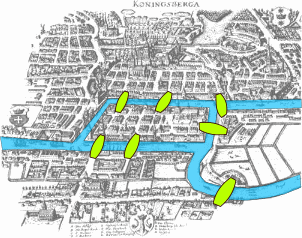
\includegraphics[width=0.3\linewidth]{Figures/Konigsberg_bridges.png} \hspace{2cm}
	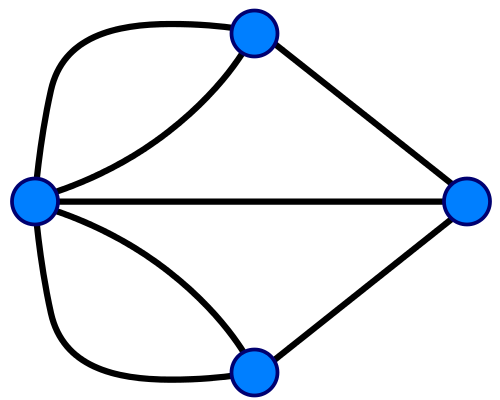
\includegraphics[width=0.3\linewidth]{Figures/Konigsberg_graph.png}
	\caption{The Kronigsber problem of seven bridges.}
	\label{fig:Krgraph}
\end{figure}

Despite the differences among complex systems, they can be represented in unique way, using graph theory. The real nature of the components is neglected, and we only represent the interaction among them. This approximation, allow us to treat equally social (graph of actors), biological (network of proteins) or even technological system (internet, traffic). In recent years complex network theory finds the application in different fields, and it's development is encored by availability of big data.

%Analyzing and Modeling Real-World Phenomena with Complex Networks: A Survey of Applications
%Characterization of Complex Networks: A Survey of measurements

\section{The structure of complex networks}

The complex system can be represented by complex network $G=(V, E)$, where the elements of system (atoms, proteins, people) map to set of $N$ nodes $V=\{1, 2, ...,N\}$. The interactions between elements map to $L$ links between nodes, $E = \{ e_1, e_2... e_L\}$. The \textbf{adjacency matrix} $\boldsymbol{A} = N \times N$ has value $1$ if there is connection between two nodes, otherwise it is $0$ \cite{boccaletti2006}. 

The network properties directly depend on the connectivity between nodes. In the case of regular networks, such as grids, each node has equal number of first neighbors. In general case, the networks have more complicated structure. Thus the important measure is network \textbf{degree} $k$. The degree of node $i$ gives the number of nodes attached to node $i$, $k_i = \sum_j A_{ij}$. The \textbf{degree distribution} $P(k)$ is probability that randomly chosen node has degree $k$. It can be calculated as fraction of $k$ degree nodes $N_k$, $p(k) = N_k/N$. The degree distribution in random network, where all nodes have the same connecting probability follows Poisson distribution $P(k)= \frac{(Np)^ke^{-Np}}{k!}$, where $k$ is mean degree distribution. In real networks degree distribution follows power law. Therefore, real networks have scale-free structure with emergence of the hubs \cite{newman2010}.

The \textbf{degree-degree correlations} in the network are measured by \textbf{assortativity}. If correlations are positive, networks are assortative; there is a tendency that connections exist between similar degree nodes. The negative correlations indicate that large degree nodes have preference to connect nodes with small degree; dissasortative networks. The average first neighbor degree $k_{nn}$ can be calculated as $k_{nn} = \sum_{k^{'}}k^{'}P(k^{'}|{k})$. The $P$ is conditional probability that an edge of degree $k$ points to node with degree $k$. The norm is $\sum_{k^{'}}P(k^{'}|k)=1$, and detailed balance conditions \cite{boccaletti2006},  $kP(k^{'}|k)P(k) = k^{'}P(k|k^{'})P(k^{'})$ \cite{boccaletti2006}. If the node degrees are uncorrelated, $k_{nn}$ does not depend on the degree, otherwise increasing/decreasing function indicates on positive/negative correlations in the network.

The Newman defined the assortativity index $r$ in slightly different way:
$r = \sum_{kl}kl(e_{kl} - q_lq_k) / \sigma_q^2$, where $e_{kl}$ is the probability that randomly selected link connect nodes with degrees $k$ and $l$, $q_k$ is probability that randomly choosen node is connected to node $k$ and equals $q_k = kp_k / \langle k \rangle$, while $\sigma_q$ is varience of the distribution $q_k$. 

The \textbf{clustering coefficient} is measure that describe the structure of neighborhood. In networks exist tendency of forming triangles or clusters. This is common in friendship networks where two friends of one pearson have high probability to be friends. The clustering can be measured by computing the number of links between neighbours of one node, $c_i=2e_i/(k_i(k_i-1))$. Averaging it over all nodes in the networks we can calculate mean clustering coefficient. It ranges from  $\langle c \rangle = 0$ where connections between neighbouring nodes do not exist, network has structure of three. On the other hand $\langle c \rangle = 1$ indicates fully connected network. 

Real world networks share similar properties. Mean distance between nodes is small and it is much smaller than number of nodes in the network $l << N$, this property is called small world phenomena. This cause the fast spread of information or even diseases in the complex systems. In small world networks number of vertices grow exponentially with distance, thus $l$ increase as $log(n)$ or slower. Logarithmic scaling can be proved from various network models, also it is observed in real world complex systems. Clustering coefficient in the real world networks is usually high. Real world networks have one important feature; power-law degree distribution; such networks are called scale-free networks.

\section{The dynamics of complex networks}

\subsection{The random graph model }

The random graph moddel was introduced by Erdos and Renyi in 1959. This model has $N$ disconnected nodes. With probability $p$ each pair of nodes can be connected.  The network is characterized only by number od nodes and links, $G(n, p)$. 

As this process is stochastic, the network with same parameters n and p, does not have to be same structure, so it is necessary to consider the ensemble of networks. Then the mean number of links depends on the model parameters:
$\langle m \rangle = n(n-1)p / 2$. The expected value of node degree can be predicted as $\langle k \rangle = (n-1)p$.
The probability $p$ is defined as density of the network. 
The probability $p(k)$ follows the binomial distribution of the form:

$p(k) = p^k(1-p)^{n-1-k}$. For large values of $n$, this becomes $p(k) = e^{-k}k^{-k} / k!$, which is Poisson distribution. 

In the case of a large random networks, the average path length is given as $l = \frac{ln n - \gamma}{ln(pn)} + \frac{1}{2}$. This means that random graph has a very small average path length. This is characteristic of many large networks. 

The clustering coefficient $C=p$, so for sparse ER graphs the clustering is very small, much smaller than in real world networks.

Increasing the probability $p$, the giant component may appear. This is sub-graph whose size is proportional to the size of the network. Such change in the network is phase-transition and it is important as small change in the probability p leads to fundamental change in the system properties. There are two limits of this model, when $p=0$, network is disconnected. If $p=1$, then network is fully connected, and giant component is with size $O(1)$.  This phenomena is related to percolation phase transition. On the threshold $p_c$, the component whose size is proportional to $n^{2/3}$ emerges. Average path length between two nodes, at critical point is proportional to the $ln N$. The small, logarithmic distance is the origin of the "small-world" phenomena. 

The interesting behavior of this model is that, with increasing p nodes tend to organise in giant component. The subcritical , $k <1$ where all components are dimple and small. The size of larges component is $s=O(ln n)$. In critical regime $k=1$, the size of largest component is $s=O(n^{2/3})$. Supercritical $k>1$, where the probability of having giant component is 1.  


\subsection{Small world networks}

In the 1999. Watts and Strogatz introduces "small-world" model. This model can generate the networks with small diameter and high clustering coefficient. Their idea is to start from grid like network, where all nodes have same number of neighbors, like ring-lattice or hexagonal lattice, where each node is connected to k nearest neighbors. Such network has high clustering coefficient, as any pair of consecutive neighbors are connected forming a triangles, while in contrast the network has high average shortest path, as nodes on the oposite sides of the lattice are not connected. The goal of this model is to connect distant nodes and reduce the average path lenght in the network. This can be simply done by randomly rewiring nodes in the network, with probability $p$. Model interpolates between regular network $p=0$ and random graph $p=1$, and for some critical probability we can achieve small world networks. 

%TODO
% mozda dodati sliku ovog moddela

The average shortest-path length from the model is close to that of an equivalent network, and much lower than that of the lattice. The clustering coefficent from the model is still close to that one in the lattice and much larger than in random network. 

The degree distribution of this model obviously is not power-law. In regular network, all nodes have equal degree, while in random networks degree distribution becomes Poisson. 

\subsection{Barabasi-Albert model}

The random network model differs from real networks in the two characteristics, growth and preferential attachment. In static models, number of nodes is fixed, while in growing models we try to simulate the continuous change in the system. More important ingredient, are linking rules. In real networks, new nodes tend to link to more connected nodes.

This model is defined as follows, we start from $m_0$ nodes, randomly connected, and at each timestep we add new node with m links that will connect to $m$ nodes already present in the network.  The probability that new node connects to node $i$ depends on node degree $k_i$ as

\begin{equation}
P(k_i) = \frac{k_i}{\sum_jk_j} 
\end{equation} 

New node can connect to any node in the network, however nodes with larger degree have higher probability to link new nodes. After time $t$ the model generates network with $N=t+m_0$ nodes and $m_0+mt$ links. Degree distribution is power-law with exponent $\gamma=3$. As network grows nodes with larger degree becomes bigger, so we end up with few nodes with many links, called hubs. Two simple mechanisms are responsible for emergence of scale-free networks. 

 \textit{degree distribution}
 
To understand the emergence of scale-free properties we need to analyze the evolution of degree distribution. The rate at which an existing node get new links as result of new nodes connecting to it is

\begin{equation}
\frac{dk_i}{dt} = mP(k_i) = m\frac{k_i}{\sum_jk_j}
\end{equation}

each new node arrives with m links. The sum is $2mt - m$ so the equation for large t becomes:

\begin{equation}
\frac{dk_i}{k_i} = \frac{1}{2}\frac{dt}{t}
\end{equation}

solving this equation we get that degree of node in time step t is $k_i(t)=m(\frac{t}{t_i})^\beta$, where $\beta=1/2$. 

We note that degree of each node increase following power-law; the growth in degrees is sub linear, as each new node has more nodes to link than previous. The eirlier node $i$, the higher is its degree. Hubs are large as they arrived early in the network. 

In summary, the analytical calculations predict that the Barabási-Al-
bert model generates a scale-free network with degree exponent 3. The degree exponent is independent of the m and m 0 parameters. The degree distribution is stationary explaining how different systems have similar structural properties. 

In summary, the absence of preferential attachment leads to a growing network with a stationary but exponential degree distribution. In contrast the absence of growth leads to the loss of stationarity, forcing the network to converge to a complete graph. This failure of Models A and B to reproduce the empirically observed scale-free distribution indicates that growth and
preferential attachment are simultaneously needed for the emergence of the scale-free property.

In the past decade we witnessed the emergence of two philosophically different answers. The first one views preferential attachment as the interplay between random events and some structural property in the network. The second assumes that each new node or link balances conflicting needs. 

The BA model postulates the presence of preferential attachment. Yet, we can build models that generate scale free networks without preferential attachment. The link selection model offers the simplest mechanism that generates a scale-free network. At each time step we add new nodes to the network, we select link at random and connect the new node to one of the two nodes at the end. The higher is degree of the node, the higher is chance that node is located at the end of chosen link. The more k-degree nodes are there, the more likely is that k node is at the end of chosen link. Probability that node at the end of randomly choosen link has degree k is $q_k = Ckp_k$. The fact that bias is linear with k indicates that the link selection model builds scale-free networks. 
Copying model can also generate scale-free networks. In each time step a new node is added to the network. To decide where it connects we randomly select node u. Then with probability $p$ new node links to $u$, otherwise with probability $1-p$ we randomly choose an outgoing link of node $u$ and link the new node to its target. The likelihood that new node connects to degree-k node is $P(k)=\frac{p}{N} + \frac{1-p}{2L}k$, the second part is equivalent in selecting a node to randomly selected link. The popularity of the copying model lies in its relevance in real systems. It is common in social networks, citation networks or even protein interactions. 
in optimization, when new nodes balance conflicting criteria as they decide where to connect

\textit{diameter}
The network diameter, represents the maximum distance in the BA model, $d \sim \frac{lnN}{lnlnN}$. The diameter grows slower than $lnN$, making the distances in BA model smaller than in random graph. The difference is found for large N. 
\textit{clustering}
The clustering coefficient of the BA model follows $C \sim \frac{ln N^2}{N}$. It is different from clustering found in random networks, and BA networks are in general more clustered. 

\subsection{Nonlinear BA model}

In summary, nonlinear preferential attachment changes the degree
distribution, either limiting the size of the hubs $(\alpha < 1)$, or leading to su-
per-hubs ($\alpha > 1$, ). Consequently, $P(k)$ needs to depend strictly lin-
early on the degrees for the resulting network to have a pure power law p k .
While in many systems we do observe such a linear dependence, in others,
like the scientific collaboration network and the actor network, preferen-
tial attachment is sublinear. This nonlinear $P(k)$ is one reason the degree
distribution of real networks deviates from a pure power-law. Hence for
systems with sublinear  the stretched exponential (5.23) should offer a
better fit to the degree distribution.


In real systems preferential attachment can be more influenced by the age of the node. If parameter alpha is negative, ageing effect overcomes the role of preferential attachment, and scale-free properties are lost. For large negative alpha, the network turns into the chain, where the youngest nodes are the most attractive. On the other hand for a positive alpha, new nodes will link to older nodes. Positive alpha makes the network more heterogeneous, and scale-free nature still exist but exponent gamma is different from 3.  for the high alpha all nodes will tend to connect to oldest node. 

In the general ageing model, we have linking rules where rules connecting probability depends on both of node degree and age difference between new and old node.  With parameters alpha and beta we can control the structure of generated networks. I already talked about some limits of the general model. We saw that for specific parameters there are SF networks, BA model, if we move from that point SF behaviour with power-law with exponent 3 is lost. And other classes of networks can appear. In general, model, when alpha and beta are both positive, rich get richer phenomena is more promoted. On the other hand, the region where beta is positive and alpha negative can be interesting, because SF networks can appear only along the critical line. 

In growing network models is considered that at each time step one node is added to the network. The remaining question is if there is any change if network growth is not linear anymore and how does it influence the structure of obtained networks.  In this work, we use numerical simulations to explore the case when $M(t)$ is a correlated time-varying function and study how these properties influence the structure of generated networks for different values of parameter $-\infty<\alpha\leq-1$ and $\beta\geq1$ and constant $L$.

\section{ Network structures}
\subsection{Bipartite networks}

A bipartite network has two partitions, $U$ and $V$. The nodes in the same partition are not connected while links exist only between nodes of a different kind. Bipartite networks represent the membership of people or items in groups. For example, we can define the network of actors as a bipartite graph. In one partition are actors and in other movies. There are no edges between actors or movies, but the actor is connected to the film if it plays in that movie. Another example is a recommender network, such as a network of people and items they like. 

The equivalent representation of bipartite network is incidence matrix $B$. If $n$ is number of people and $g$ number of groups, this matrix is $g x n$, having elements $B_{ij}$ 1 if persoon i belongs to group j. 

Even bipartite networks give realistic representation of the system, there is often need to analyze the single type of nodes.  From a bipartite network, we can generate two projections. The first one connects nodes partition $V$ if they point to node $u$. Similarly, we can project the network on U partition, connecting $u$ nodes. The one mode projection between actors and movies onto actors is undirected network of actors. Actors are connected if they appear in the same movie. We can also create one-mode projection onto movies, where two movies are connected if they share the same actor.  

The projections are useful in some manner, but they also lose some important information, for example how many groups nodes share in common. This information can be propagated adding the weight to the edges, equal to the number of common groups.

The product $B_{ki}$ and $B_{kj}$ is 1 if $i$ and $j$ belong to the same group $k$. Thus the total number of groups to which nodes $i$ and $j$ belong is 

$P_{ij} = \sum_{k=1}^g B_{ki}B_{kj} = \sum_{k=1}^g B_{ik}^TB_{kj}$. The matrix $P$ is matrix of one-mode projection. The diagonal elements are non-zero, and represent the number of groups node $i$ belongs to.  To derive the weighted adjacency matrix, the diagonal elements are set to 0. The adjacency matrix of unweighted projection, each non-zero element needs to be replaced with $1$. 

\subsection{Core-periphery networks}

Core-periphery structure describes a network whose nodes are divided into two community, densely connected core and less connected periphery. If we consider the average probabilities of edges within each group as $p_{11}$ and $p_{22}$, and between groups $p_{12}$, instead of traditionaly assortative or dissasortative structure we can define core-periphery structure $p_{11}> p_{12} > p_{22}$. In the principle core-periphery structure does not have to be limited to only two groups, and we can define layered, onion, structure. The network can have more cores, that are not directly connected to each other. 

The simple method for finding core-periphery structure is to assume that nodes in core have higher degree in the core than in the periphery. Another simple method is to construct k-cores. K core is group of nodes that each has connection to at least k other members of the group. K-cores form a nested set, and become denser with higher k. The core-periphery structure can be detected optimizing the measure similar to modularity, as defined by Borgatti and Everett. Their goal is to find the division that minimizes the number of edges in the periphery. So they define the score function that is equal to number of edges in the periphery minus the expected number of such edges placed at random. $\rho = \frac{1}{2}\sum_{ij}(A_{ij}-p)g_ig_j$. They used genetic algorithm to minimize this function. 

The another way to detect core-periphery structure is to use the inference method based on fits to a stochastic block model. In this method we fit observed network to a block model with two groups, such that edge-probabilities have form $p_{11}> p_{12} > p_{22}$. The only downside of this model is that method is going to find the structure that optimize likelihood, and we can not say weather it is core-periphery or community structure. 

\subsection{Communities}

Thus the ability to find groups or clusters in a network can be a useful tool for revealing structure and organization within networks at a scale larger than that of a single node or a
few nodes. The occurrence of groups or communities is not limited to social networks.
Clusters of nodes in a web network, for instance, might indicate groups of
related web pages. Clusters of nodes in a metabolic network might indicate
functional units within the network. The ability to find groups also has another practical application: it allows
us to take a large network and break it apart into smaller subsets that can be
studied separately. The network in Fig. 14.1 is quite small, but others may be
much larger, millions of nodes or more, making their analysis and interpreta-
tion challenging. Breaking such networks into their component clusters is a
useful technique for reducing them to a manageable size. One example of this
approach is in network visualization. A network with a million or more nodes
can rarely be visualized in its entirety, even with the aid of good visualization
software. Such networks are simply too big to be represented usefully on the
screen or on paper. If the nodes of the network divide naturally into groups,
however, then we can make a simpler but still useful picture by representing
each group as a single node and the connections between groups as edges.
An example is shown in Fig. 14.2. This simplified representation allows us to
see the large-scale structure of the network without getting bogged down in
the details of the individual nodes. If one wanted to see the individual nodes,
one could then “zoom in” to a single group and look at its internal makeup. The problem of finding groups of nodes in networks is called community
detection. Simple though it is to describe, community detection turns out to be
a challenging task, but a number of methods have been developed that return
good results in practical situations.

\subsection{Stochastic block model}
The network or graph is the structure of nodes and edges, where each edge connects two nodes. Nodes can be organized into groups, called communities. Identifying these hidden blocks can lead to interesting insights into the network. However, the community detection problem does not give a precise definition of what a community is. As a consequence, many approaches try to recover such structural patterns in the network \cite{martin}.

A common definition of a community is that it is densely connected subgraph \cite{userguide}. We can find these subgraphs by optimizing an objective function, such as modularity function. It measures the difference in the number of edges between the given network and the network with the same number of nodes but randomly connected. In this approach, we try to maximize the density of connections inside a group by focusing more on assortative\footnote{Networks where nodes tend to connect with other nodes of a similar degree. Edges are more likely inside blocks than out of them.} group structures. 

Another type of networks is the bipartite network that has two disjoint sets of nodes. The edges exist only between nodes from different sets. Networks of this class can appear in real-world data, such as users-movies preference, collaboration network for scientists and papers, etc. Application of density-based approach requires to first project bipartite network to one of its partitions and then find communities in that projection. With this, some information is lost. On the other hand, the method that is directly applicable to bipartite networks is Stochastic Block model, from which the models considered in this paper are derived.

Stochastic block model (SBM) is based on connection probabilities between nodes. It is a generative model which includes existence of communities. Parameters that describe SBM for network G with N nodes are:

\begin{itemize}
	\item k: number of groups
	\item group assignment vector, g: $g_i \in\{1,2..k\}$, gives the group index of node $i$.
	\item SBM matrix, $p_{k \times k}$, whose elements $p_{ij}$ are the probabilities that edges between groups $g_i$ and $g_j$ exist.
\end{itemize}

Note that nodes within one group have the same connection probabilities.

SBM can generate and describe different types of network structures. Figure \ref{fig:SBM} \cite{userguide} shows how the model matrix corresponds to resulting networks with two communities. First, for the assortative network (\ref{fig:SBM} a), diagonal elements of the matrix have higher probabilities. This indicates dense connections inside the group, just like in classic community structures. In disassortative structure, (\ref{fig:SBM} b), more connections exist between two partitions than inside them, i.e. off-diagonal elements have higher probabilities. Bipartite networks can be represented like this. 

Figure (\ref{fig:SBM} c) shows how the model represents core-periphery networks. Nodes of one block (core) are well connected with itself and with other partition (periphery). From the last case, we can note that SBM with one group is the Erdos Renyi random graph (\ref{fig:SBM} d) because all probabilities inside and between groups are equal.

The benefit of this model is that we can generate many networks with similar group structure. The model can fit real data, which results in finding network communities. For the given network $G$ and number of groups $k$, the best nodes partition $g$ is found by maximizing the likelihood function. Beside inferring communities, SBM has application in prediction of missing links. This simply formulated model has many variants, motivated by specific properties of real data. For example, for networks which are degree heterogeneous, there is degree corrected SBM. In some social networks, users can belong to more than one group, and this can be modelled with mixed membership SBM. Other extensions include application to bipartite, weighted network, hierarchical model, etc. Also, several algorithms for optimization of likelihood function are proposed. The overview of these versions and methods are given in \cite{comparison}. In this paper, we will focus on Single and Mixed Membership SBM applied on bipartite networks.  
\begin{figure}
	\centering
	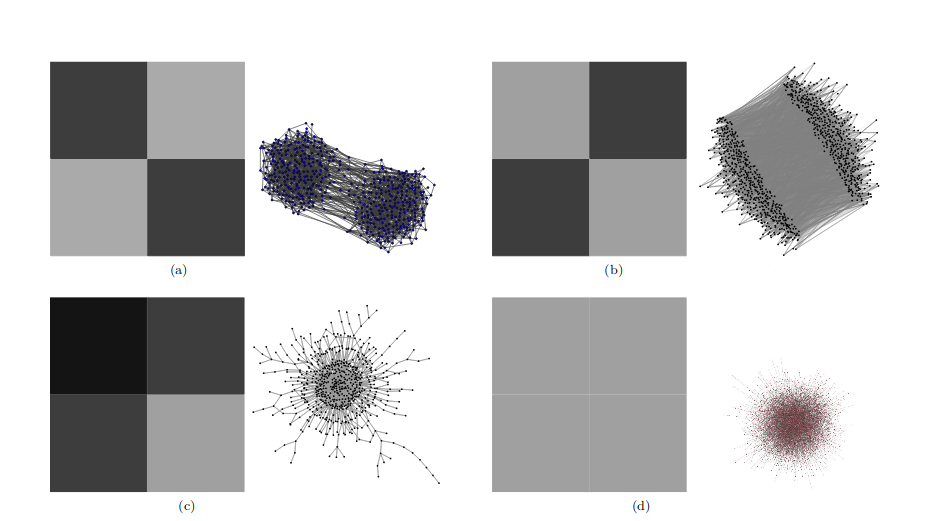
\includegraphics[width=0.7\textwidth]{Figures/structures.png}
	\caption{Stochastic Block model for different networks structures. (a) assortative. (b) dissortative. (c) core-periphery. (d) Erdos Renyi random graph.}
	\label{fig:SBM}
\end{figure}


\section{Graph isomorphism}

Weisfeiler-Lehman Test

\section{Distributions}

\subsection{power-law}
Power-law distributions characterize many social and biological systems. Power-law distributions are also easy to generate. 

the distributions: basic definitions and properties

The nonnegative random variable X is said to have a power law distribution if 
\begin{equation}
Pr[X>x] \sim c x ^{-\alpha}
\end{equation}

for constants $c>0$ and $\alpha >0$. In power-law distribution asymptotically the tails fall according to power $\alpha$. Such distribution leads to much havier tails than other common models, as exponential distribution. 

One specific power-law distribution is Pareto distribution which satisfies 

\begin{equation}
	Pr[X>x] = \frac{x}{k} ^{-\alpha}
\end{equation}

for some $\alpha>0$ and $k>0$. The Pareto requires $X>k$. The density function of Pareto distribution is $f(x)=\alpha k^\alpha x^{-\alpha-1}$. For power law distribution $\alpha$ is in the range $0 < \alpha < 2$, in which case X has infinite variance, if alpha <1 X has infinite mean.

if X has power law distribution, then a in log-log plot $Pr(x)$ will behave as straight line. For the specific case of Pareto distribution, the behaviour is exactly linear as $ln (Pr(x)) = -\alpha (lnx -ln k) $. Similarly the density function is also straight line. $ln(f(x)) = (-\alpha - 1) ln (x) + \alpha ln (k) + ln(a)$

\subsection{log-normal}
Many measurments in the nature show a more or less skewed distribution. They are common when mean values are low, variances are large and values can not be negative as example in distribution of minearal resources in the Eart. Such skewed distributions often closely fit to log-normal distribution. 

What is the difference between normal and lognormal variability? A major difference is that effect can be additive or multiplicative, leading to normal or lognormal distribution. Basic principles of additive and multiplicative effects can be easily demonstrated with the help od two dices. Adding the two numbers, which is the principle of the most games, leads to values from 2 to 12 with mean of 7, and simetrical frequency distribution. Multiplying the two numbers, leads to values from 1 to 36 with highly skewed distribution. Although these examples are not normal or lognormal they give us clear difference how different distributions can emerge. 

Log-normal distributions are usually characterized in the term of the log-transformed variable, using as parameters the expected value, or the mean, and the standard deviation. This characerization can be advantageous as by definition log-normal distributions are simetrical at the log level. 

The basic properties of the lognormal distributions

Random variable $X$ if $log(X)$ is normally distributed., if $Y=ln X$ has normal Gaussian distribution.  

Only positive values are possible for the variable and distribution is skewed. Two parameters are needed to specify lognormal distribution. Traditionaly the mean $\mu$ and standard deviation $\sigma$ or the variance of the $\sigma^2$ of $log(X)$ are used. However there are clear advantages of using transformed data, $\mu^{*} = e^{\mu}$, $\sigma^{*}= e ^{\sigma}$. The median of this lognormal distribution is $med(X)=\mu^{*}=e^{\mu}$, since $\mu$ is median of the $log(X)$.

\begin{equation}
f(x) = \frac{1}{x \sigma \sqrt{2\pi}}exp(-\frac{1}{2\sigma^2}(log(x)-\mu)^2)
\end{equation}

The mean is $exp(\mu + \sigma /2)$ and variance is $(exp(\sigma^2)-1)exp(2\mu+\sigma^2)$. 

Estimation: The asymptotically most efficient (maximum likelihood) estimators are 
\begin{equation}
x* = exp (\frac{1}{n}\sum_{i=1}^n log(x_i)) = (\prod_{i=1}^nx_i)^{\frac{1}{n}}
\end{equation}

\begin{equation}
s* = exp([\frac{1}{n-1}\sum[log(\frac{x_i}{x*})]^2]^{\frac{1}{2}})
\end{equation}


The lognormal distribution is skewed with mean $e^{\mu + \frac{1}{2}\sigma^2}$, median $e^\mu$ and mode $e^{\mu - \sigma^2 }$. It has finite mean and variance, in contrast to the power-law distribution.  

Despite it has finite moments, the lognormal distribution can be similar to power-law. If $X$ has a lognormal distribution then loglog plot of density function can apear as straight line for a large portion of a body of distribution. If the variance is large, the distribution may appear linear on log-log plot for several orders of magnitude. The variance of the corresponding normal distribution is large, the distribution may appear linear on a log-log plot. To see this we can check the logarithm of density function. 
If $\sigma$ is large then the quadratic term will be small for large range of x values, so the logarithm of the density function will appear almost linear for large range of values. 
Recall that normal distribution have property that the sum of two independent normal variables is normal variable. It follows that product of two lognormaly distributed random variables also has a lognormal distribution. 

\section{Scale-free networks}

The study of scale ivariance has a long tradition. Among the fields where this property was analysed were the theory of critical phenomena, percolations and fractal geometry. One of the first examples considered eas the price fluctuations  of cotton in commodities market (Mandelbort, 1963). The future price can not be obtained with arbitary precision from past series., still this series have some form of regularity. The curves for daily, weakly and montly price fluctuations are statistically similar. The fact that some features are found at different time scales is typical sign of fractal behaviour. Similarly in the case of coastline lenght we find fractal behavior. If we try to measure the total lenght, the real shape is so complicated that we always miss some part. 

Fractal behaviour might refer to different properties. In some systems scale-free structure is in shape. In this class the fractal shape can be robust, as in the case of branched patterns or electric breakdown. We say robust because these phenomena happen for varaity of external conditions. In the same class we have other systems that are more fragile, in the sense that they arise after precise tuning of some physical quantity. This is in the case of percolations and critical phenomena. Scale-free invariance may be related with dynamics or evolution of the system. The time activity of the system may display self-similar behaviour. The only sign of fractal behaviour is the mathematical form, power-law fluctuations of the time-series. 

The self-similarity can be present in the way the different parts of a system interact with each other. This is the case with self-similar graphs and the power-law scaling appers in the distribution of topological quantities like the number of interactions per part  of the system. These phenomena are fractals in the topology. 

\section{Scale-invariance and power laws}

The mathematical form of self similarity is represented by powe-laws. Whenever the function $y = f(x)$ can be represented as a constant to the power of x. The physical example is elastic force, the gravitational and electrostatic force. In the case of fractals, their geometry can be identified by considering the numbe of boxes $N(\epsilon)$, of linear size $1/\epsilon$. $N(\epsilon) = \epsilon ^{-D}$, where D is called fractal dimension. D can also be defined using mass relation $M = L^ D$.

Scale invariance is not restrected to geometry, but also appears in dynamical systems. In this case we have power-law distribution for different physical quantities. For example the evolution of some systems (sanspiles, number of species in the ecosystem) proceeds  with series of causally connected events whose size s is distributed as power-law. $P(s) s^{-\tau}$.

\subsection{plotting a power-law}

if we plot the data on double logarithmic scale, we should obtain a straight line. $y = x^{\alpha}$, $ln(y) = \alpha ln(x)$. The tail of the distributon is very noisy, and it is general feature of many experiments. To avoid the fluctuations in the tail it is common to use "binning" or cumulative distribution. 

In this method the noise reduction is done by deviding the $x$ axis into bins, and averaging the data within each bin. As an example we can take the frequency of numbers between numbers $1$ and $10$. Let assume that bin is $10$ units wide, we can represent all data in one point $b$, with $xb$ given by average of the bin extremes and $yb$ given by the avarage value of $ys$. If the bin size is constant for large values of $x$ the density of bins becomes very large as well. 

In the case of powerlaws it is usufull to use logarithmic binning. For example take the size of the first bin to be 2, and the others are power of 2. $2^1, 2^2...$. A possible choice is to take as yb the average of the values ys in the bin, and as xb the geometrical average of the bin extremes. Bins are equaly spaced on logarithmic scale. The base can be any number larger than 1, for example 1.2. The drawbacks of this procedure are following: this method does not complitly reduce the noise and the choice of the most appropiate bin size must be determined by using trial and error. In general, small and noisy dataset , the behavior in the tail of distribution can be lost if the bins are too wide. Too small bins will not average the present fluctuations

Using the method of cumulative distribution instead of calculating the probability that certain value x appears in the experiment, we focus on the probability that an outcome is larger than x. 

For power-law, 
%$P>(x) = \int_{x}^{\inf} P(x^{'})dx^{'}$.
 For power law cumulative distribution is still powerlaw but with modified exponent. $-\alpha+1$. Still, in this method, if exponent is close to one, integral does not behave like powe-law, reather logarithm. The upper limit is a finite value $x_{max}$ and this can change the shape of curve. 

The cumulative distribution will resemble a power law only as the value of $xmax$ tends to infinity. Otherwise, the deviation from the straight line could make estimating the exponent very difficult.


\subsection{multiplicative processes}

While many power laws are originated by some ‘complex’ mechanism, some
others have a very simple explanation. By using multiplicative processes we
can obtain quite naturally both power laws and log-normal distributions
(that can look like power laws) (Goldstein, Morris, and Yen, 2004). We
do not enter here into the debate over whether observed data can be best
fit by power law or log-normal variables. Here it is enough to note that
the mechanism of multiplicative process is probably the most immediate
model for fat-tail phenomena in nature since it naturally produces both.

Many textbooks and scientific papers deal with this topic. Some of them
are very beautiful and complete and we suggest them for further reading
(e.g. Mitzenmacher 2004; Newman 2005). Suppose you have an evolution
process, where for example an organism transforms itself in time. As a
general statement, the state S t at time t will be determined by the previous
states and by the external conditions. Whenever the state of the system can
be written as we have a multiplicative process. In other words, in a multiplicative process,
the state of the system at time t is proportional to the state at time t-1. In
biology this could represent the fact that the growth of an organism is ruled
by its body mass at the previous step. In the case of city growth (Zanette and
Manrubia, 1997; Manrubia and Zanette, 1998; Gabaix, 1999) this equation
states that the population at a certain time step is proportional to what
it was previously. In both cases the proportionality constant is given by
the factor t that can change its value at any time step. Turning back to
eqn 4.114 we can immediately see that the variable S t is determined by the
product of the various tau where tau is between 0 and t This sum of the logarithms of the tau (under very mild conditions) is a variable following a normal distribution (regardless of the distribution of the tau ).
This result comes from the application of the ‘central limit theorem’. This
theorem states that, in certain very general hypotheses, the sum of identi-
cally distributed random variables with finite variance is a new stochastic variable normally distributed. Therefore, if ln(S t ) is normally distributed,
the variable S t is log-normally distributed. This very simple mechanism has been rediscovered and explained over
and over many times since the definition of log-normal distributions in 1879
(McAlister, 1879). One of the first applications of these ideas traces back at
least to the economist Gibrat (1930, 1931) who uses essentially this model
under the name of proportionate effect. Using a different terminology, a
somewhat similar idea was introduced at the beginning of last century for
biological problems (Kapteyn 1903, 1918).
With this idea we have two possible outcomes. As explained above we
have true log-normal distributions that can easily be confused with power
laws. This happens whenever the log-normal distribution is studied in a
range of k for which $\sigma >> ln(k)$. On the other hand, a very similar situ-
ation also triggers the formation of true power laws as shown in the next
subsection. Powerlaws from multiplicative processes.

\section {Preferential attachment}

One of the most successful applications of multiplicative processes is given
by preferential attachment. To date, this is the most successful mechanism
adopted in the study of growing networks. Interestingly, the idea that we
are going to explain has been independently rediscovered several times in
different fields and ages. Precisely for this reason it has also been given
several names. For example: Yule Process, Matthew effect, Rich gets richer,
Preferential Attachment, Cumulative advantage.
In the community there is some agreement (Mitzenmacher, 2004; New-
man, 2005) that the first to present this idea has been G. Yule (1925) in
order to explain the relative abundance of species and genera in biological
taxonomic trees. As shown in Chapter 8 when considering a set of biolog-
ical species we have that the classification (taxonomic) tree has scale-free
properties. The null hypothesis consists in considering that the set of species
arises from a common evolution. Therefore we consider one parent species
and after mutation we obtain a new one that very likely can be grouped
in the same genus. Every now and then though, speciated species (the new
ones) can be so different from the parent one that they can form a new genus
on their own (or be grouped in an existing different one). The probability
of speciating will be larger for genera that are already large, since mutation
rate is constant for any individual.
This explanation allow us to focus on the two ingredients of the model.
Firstly you have to invoke a certain a priori dynamics (hereafter called
growth). Secondly, this dynamics selects successful elements and makes
them even more successful (hereafter called preferential attachment). In
detail, take a set of elements each of which is characterized by a certain
number N i t . As a possible example this could be the number of different
genera that have i species per genera. The set can also be a set of vertices
in a graph and the number N i t can represent the number of pages whose
in-degree is i. Now let us introduce a rule that introduces new elements in
the set; these elements will not be shared equally between the older ones,
but rather will be assigned more to those that already have many. Let us
consider that N i t gives the number of vertices with certain degree i (the total
















\section{In This Thesis}




% Chapter 1

\chapter{Driving signals} % Main chapter title

\label{Chapter2} % For referencing the chapter elsewhere, use \ref{Chapter1} 

% Define some commands to keep the formatting separated from the content 

%----------------------------------------------------------------------------------------

% Define some commands to keep the formatting separated from the content 

The complex networks grow through the addition of new nodes, and growing networks models consider that growth is constant over time. This approximation is sufficient for explaining how properties of complex networks can emerge; for example, in the Barabasi-Albert model such as in real systems, we find scaling of degree distribution. Models mostly focus on linking rules and their influence on the topology of complex networks. 

Still, the growth of real systems changes over time. In online social networks, new users join on daily basis and the users' activity might have bursty nature. We can consider a co-authorship network, where links are created between scientists when they publish a paper. The dynamic of real networks can be complex and highly influenced by non-linear signals. The growth signal; the number of new nodes in each time step; has cycles and trends. Circadian cycles are directly reflected into growth signals and we also find long-range correlations and multifractal properties. 

In this chapter, we explain the properties of growth signals, both real and computer-generated. We analyze networks created with a growing network model where the interplay between ageing and preferential attachment shape their structure. We are interested to incorporate non-constant growth signals into the model and measure their impact on the complex networks. Differences between networks with the same number of nodes and links can be observed through connectivity patterns. Figure \ref{fig:ciljevi} describe used model. 
   

\begin{figure}[!ht]
	\centering
	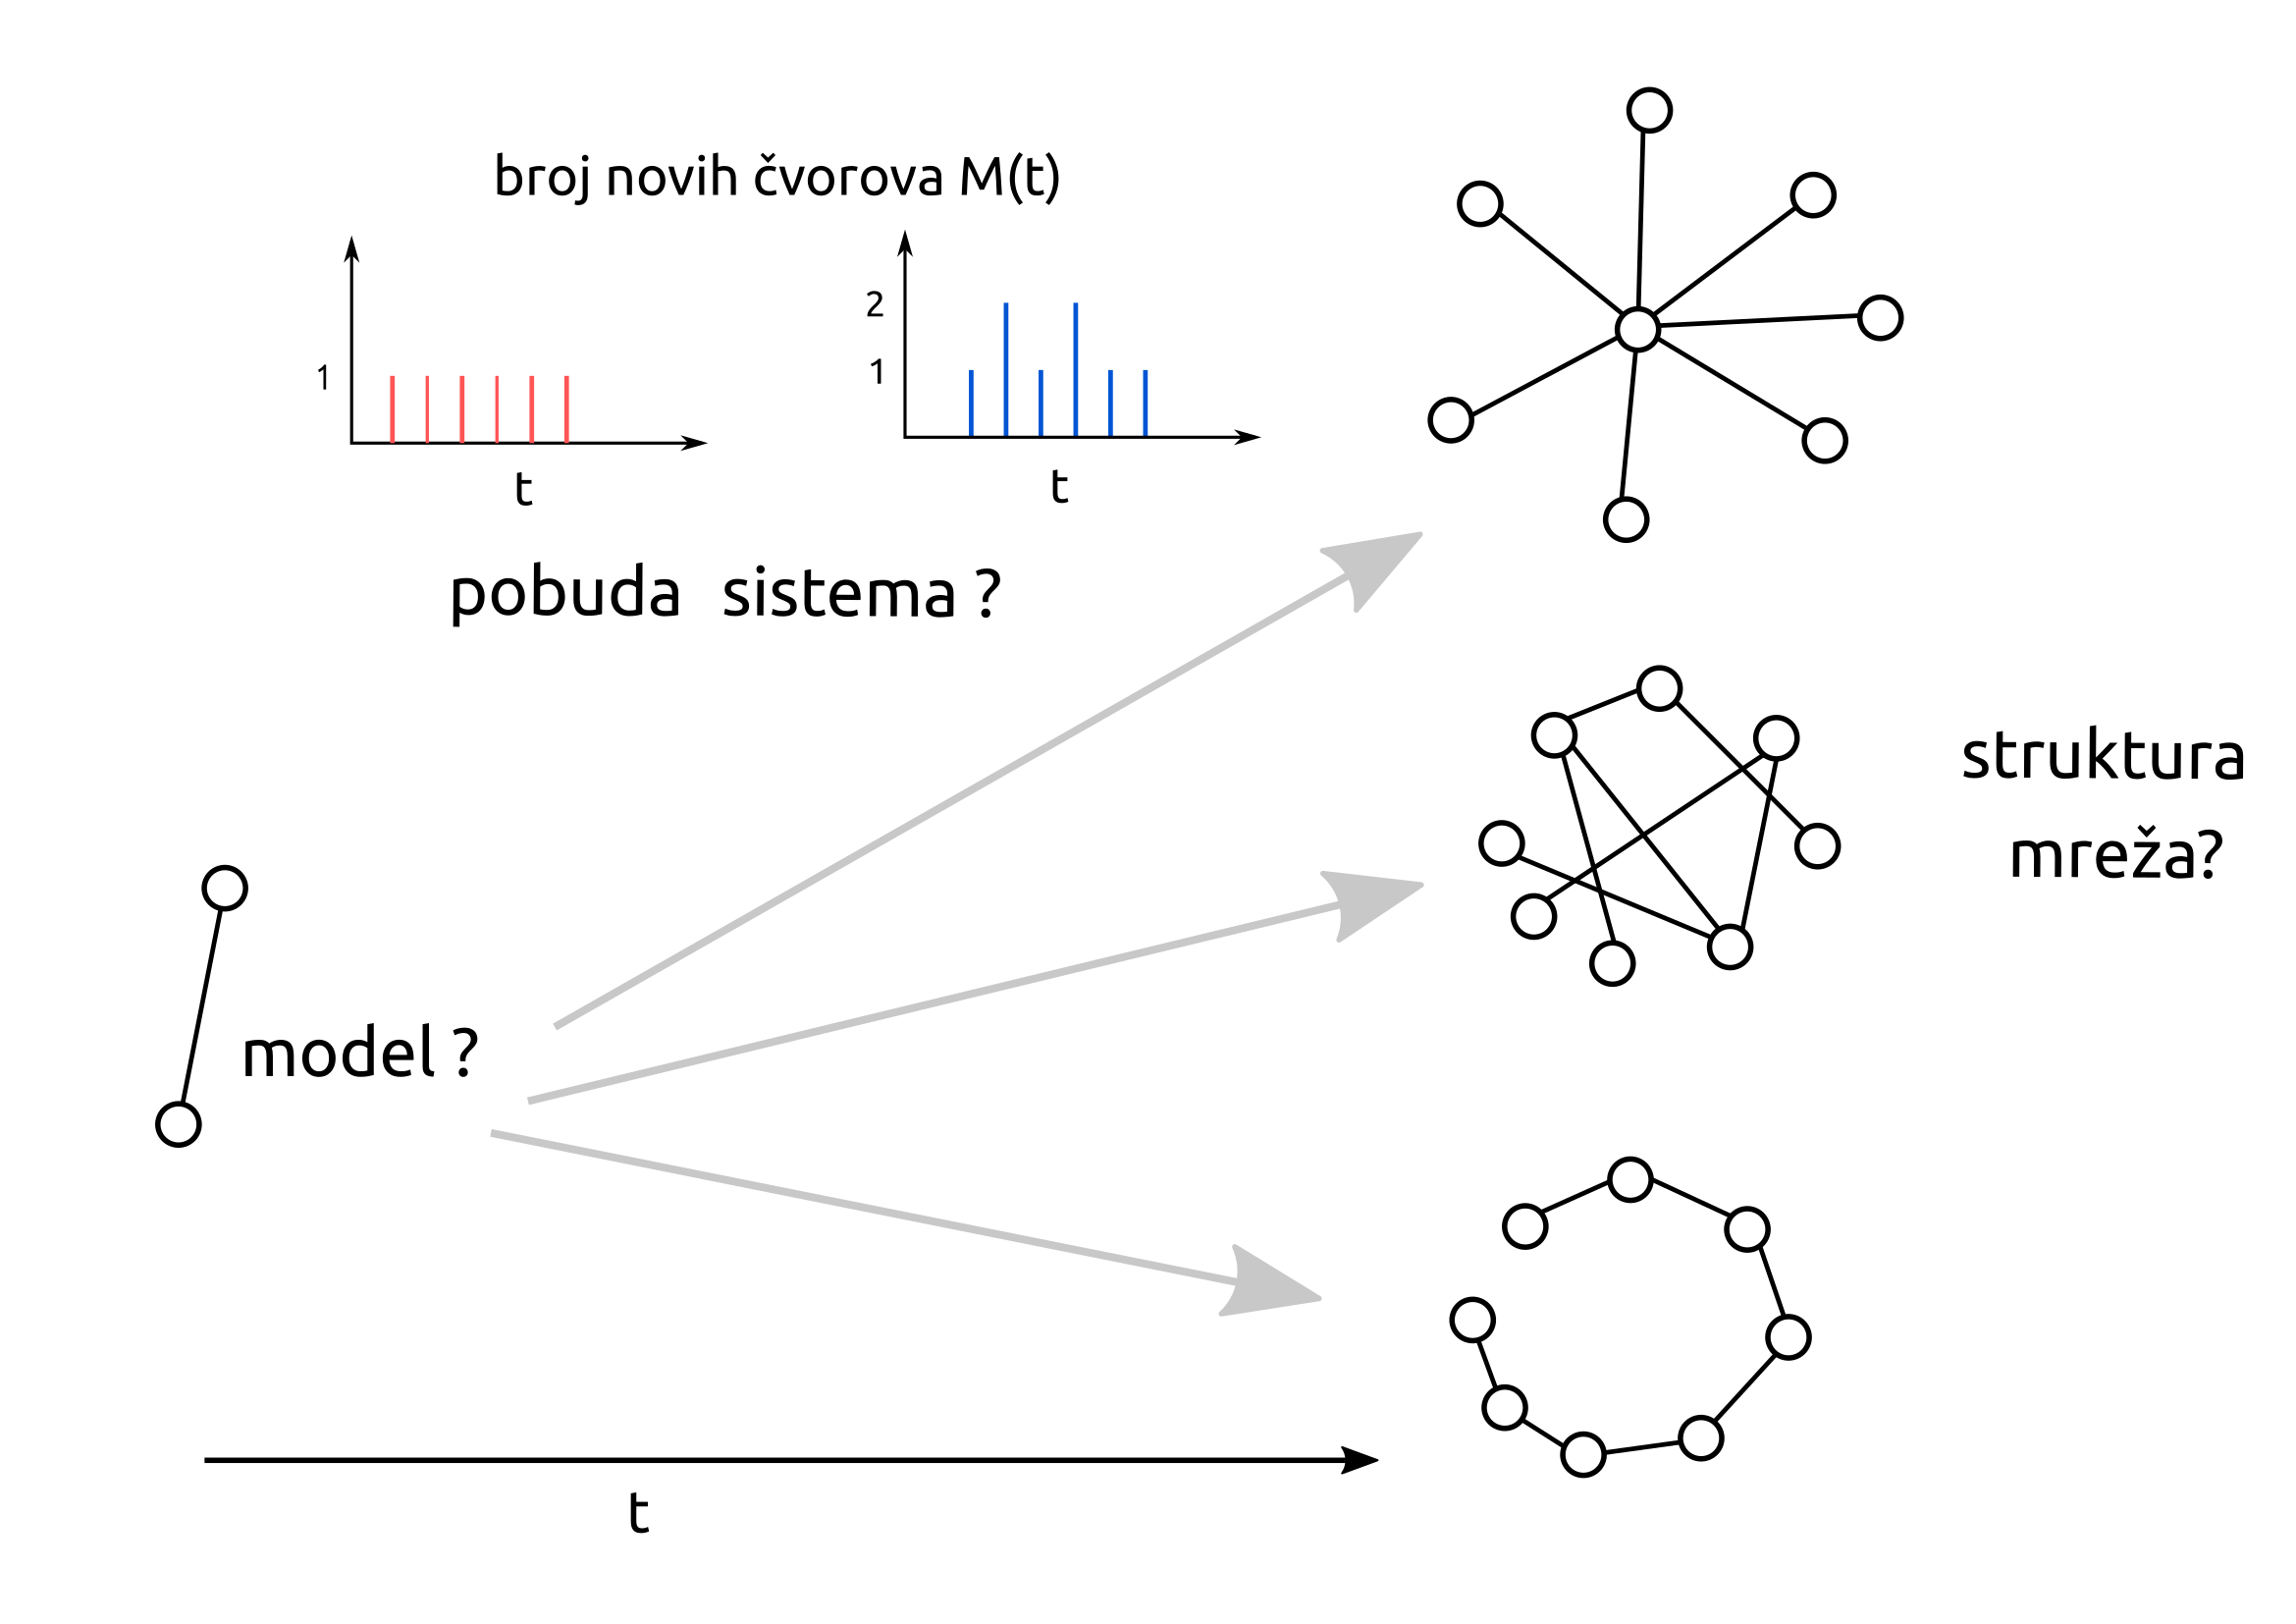
\includegraphics[width=0.6\linewidth]{Figures/ciljevi3.png}
	\caption{Growing network model schema.}
	\label{fig:ciljevi}
\end{figure}

\section{Growing signals}

\subsection{Long range correlated signals}

The main characteristic of long-range correlated time series is power law decay of autocorrelaction function, $C(s)= <x_i x_{i+1}> = s ^ {-\delta}$. Instead of using correlation function to directly determine type correlations in the signal, in practice is more common to calculate Hurst exponent.  

Hurst exponent is used for estimating self-similarity of the time series described with relation $x(ct)=cHx(t)$. Hurst exponent and autocorrelation coefficient $\delta$ are connected  as  $H = 1- \frac{\delta}{2}$. When $H=0.5$ signal has short range correlations and is considered to be white noise, while for $H=1.0$ signal is pink noise. Between this limits $0.5<H<1.0$, signal has long range correlations.

Monofractal signals can be generated using Fourier transform method \cite{makse1996method}:
\begin{itemize}
	\item first generate one-dimensional sequence of uncorrelated random numbers $u_i$ from Gaussian distribution with $\sigma=1$
	\item calculate the Fourier transform of the generated sequence, $u_q$
	\item filter signal $x_q = u_q s$, where $s$ is Fourier transform of autocorrelation function $C(s)$ 
	\item the inverse Fourier transform $x_i$ is signal with specific long range correlations 
\end{itemize}     

\begin{figure}[h!]
	\centering
	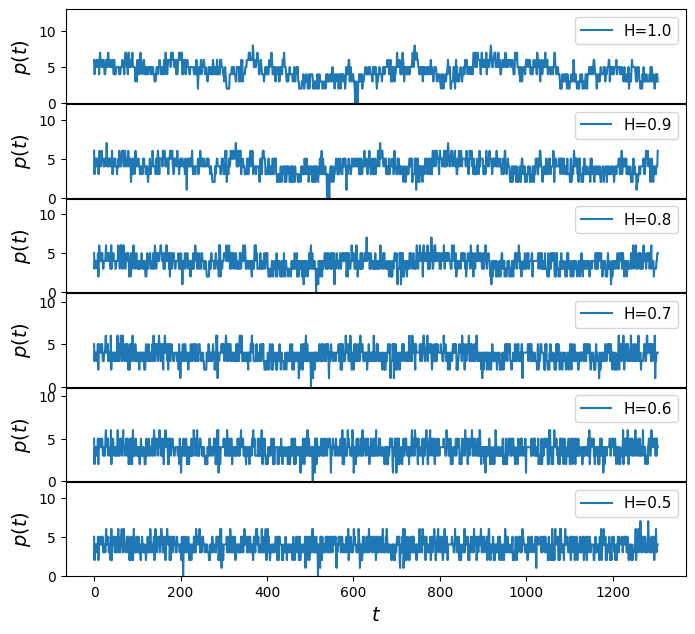
\includegraphics[width=0.7\linewidth]{Figures/monofractals.png}
	
	\caption{Monofractal signals}\label{fig:monofractals}
\end{figure}

Figure \ref{fig:monofractals} shows artificial signals generated using Fourier transform method for different values of Hurst exponents. The obtained signals are round to integers, as in real time series integer values are present. The mean values of signals are close to $4$.

For estimation of Hurst exponent from non-stationary signal can be used detrended fluctuation analasys (DFA) \cite{kantelhardt2001} \cite{peng1994}. This method removes trends and cycles from the signal, while Hurst exponent is estimated based on residual fluctuations. Signals from real world have usually  multifractal structure and can not be described with only one value of Hurst exponent \cite{kantelhardt2002}

\subsection{Multifractal analysis}

Multifractal detrended fluctuation analysis (MFDFA) \cite{kantelhardt2002, ihlen2012} to estimate multifractal Hurst exponent H(q). For given time series $\{x_i\}$ with length N, first we define global profile in the form of cumulative sum, equation \ref{eq:cumsum}, where where $\langle x\rangle $ represents average of the time series:
\begin{equation}
Y(j) = \sum_{i=0} ^j (x_i - \langle x\rangle), \quad j=1, ..., N
\label{eq:cumsum}
\end{equation}

Subtracting the mean of the time series is supposed to eliminate global trends. The profile of the signal Y is divided into $N_s = int (N/s)$ non overlapping segments of length s. If $N$ is not divisible with s the last segment will be shorter. This is handled by doing the same division from the opposite side of time series which gives us $2N_s$ segments. From each segment $\nu$, local trend $p^m_{\nu, s}$ - polynomial of order m - should be eliminated, and the variance $F^2(\nu, s)$ of detrended signal is calculated as in equation \ref{eq:var}:
\begin{equation}
F^2(\nu, s) = \frac{1}{s}\sum_{j=1}^s \left[Y(j) - p^m_{\nu, s}(j)\right]^2
\label{eq:var}
\end{equation}
Then the q-th order fluctuating function is: 
\begin{equation}
F_q(s) = \left\{\frac{1}{2N_s}\sum_{\nu}^{2N_s}\left[F^2(\nu, s)\right]^{\frac{q}{2}}\right\}^{\frac{1}{q}},  q \neq 0 \nonumber
\end{equation}
\begin{equation}
F_0(s) = \exp \left\{\frac{1}{4N_s}\sum_{\nu}^{2N_s}ln \left[F^2(\nu, s)\right]\right\}, q=0
\end{equation}

The fluctuating function scales as power-law $F_q(s) \sim s^{H(q)}$ and the analysis of log-log plots $F_q(s)$ gives us an estimate of multifractal Hurst exponent $H(q)$. Multifractal signal has different scaling properties over scales while monofractal is independent of the scale, i.e., H(q) is constant. 

\subsection{Real signals}

In this work, we use two different growth signals from real systems figure 1: (a) the
data set from TECH community from Meetup social website [36] and (b) two months
dataset of MySpace social network [37]. TECH is an event-based community where
members organize offline events through the Meetup site [36]. The time unit for TECH
is event since links are created only during offline group meetings. The growth signal
is the number of people that attend the group’s meetings for the first time. MySpace
signal shows the number of new members occurring for the first time in the dataset [37]
with a time resolution of one minute. The number of newly added nodes for the TECH
signal is N = 3217, and the length of the signal is T = 3162 steps. We have shortened
the MySpace signal to T = 20221 time steps to obtain the network with N = 10000
nodes.
\begin{figure}[!ht]
	\centering
	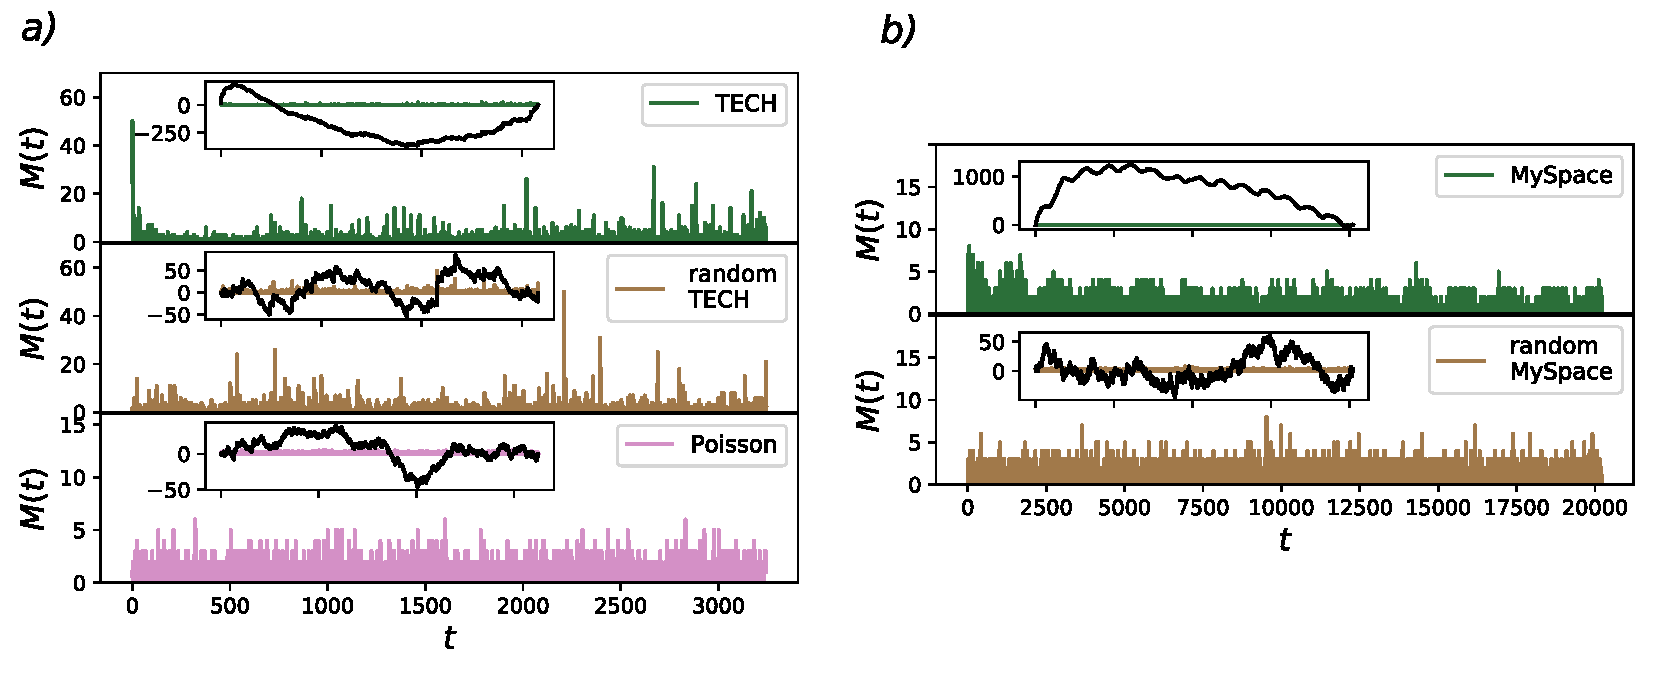
\includegraphics[width=\linewidth]{Figures/signals.pdf}
	\caption{Growth signals for TECH (a) and MySpace (b) social groups, their randomized counterparts, and random signal drawn from Poasonian distribution with mean $1$. The cumulative signals are shown in insets.}
	\label{fig:signals}
\end{figure}

\begin{figure}[!ht]
	\centering
	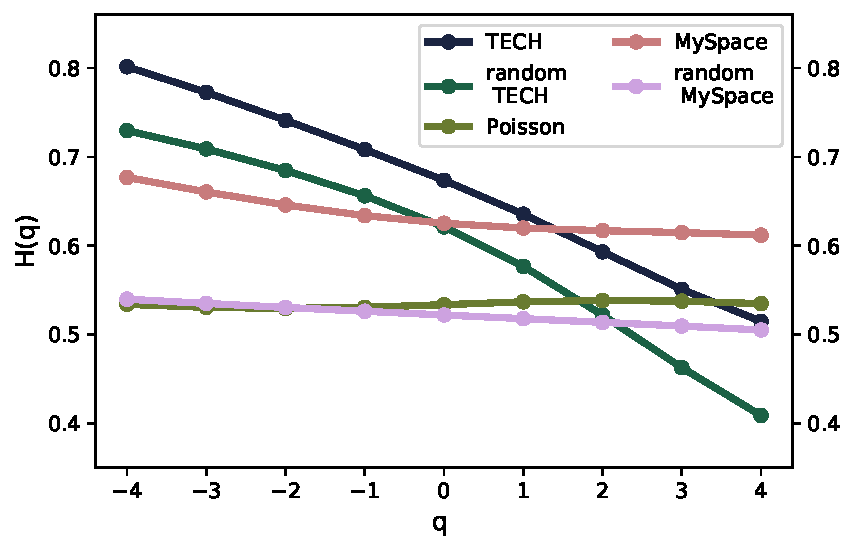
\includegraphics[width=0.6\linewidth]{Figures/hurst.pdf}
	\caption{Dependence of Hurst exponent on parameter $q$ for all five signals shown in figure \ref{fig:signals} obtained with MFDFA. }
	\label{fig:mfdfa}
\end{figure}
Real growth signals have long-range correlations, trends and cycles [37, 27, 25]. We
also generate networks using randomized signals and one computer-generated white-
noise signal to explore the influence of these signal’s features on the structure of
evolving networks. We randomize real signals using reshuffling procedure and keep their
length and mean value, the number of added nodes, and probability density function
of fluctuations intact, but destroy cycles, trends, and long-range correlations. Besides,
we generate a white-noise signal from a Poissonian probability distribution with a mean
equal to 1. The length of the signal is T = 3246, and the number of added nodes in the
final network is the same as for the TECH signal.

Figures \ref{fig:signals} (a) and \ref{fig:mfdfa} show that the TECH signal has long trends and a broad probability density function of fluctuations. The trends are erased from the randomized TECH signal, but the broad distribution of the signal and average value remain intact. MFDFA analysis shows that real signals have long-range correlations with Hurst exponent approximately $0.6$ for $q=2$, figure \ref{fig:mfdfa}. The TECH signal is multifractal, the consequence of both broad probability distribution for the values of time series and different long-range correlations of the intervals with small and large fluctuations. Shuffling of the time series does not destroy the broad distribution of values, the reason for the persistent multifractality of the TECH randomized signal, figure \ref{fig:mfdfa}.

MySpace signal has a long trend with additional cycles that are a consequence of human circadian rhythm, figure \ref{fig:signals}(b). It is multifractal for $q<0$, and has constant value of $H(q)$ for $q>0$, figure \ref{fig:mfdfa}. In MFDFA, with negative values of $q$, we put more emphasis on segments with smaller fluctuations, while for positive $q$ emphasis is more on segments with larger fluctuations \cite{ihlen2012}. Segments with smaller fluctuations have more persistent long-range correlations in both real signals, see figure \ref{fig:mfdfa}. Randomized MySpace signal and Poissonian signal are monofractal and have short-range with $H=0.5$ correlations typically for white noise.    


\section{Growing network model with aging nodes}

%The model starts with small number of nodes randomly connected. Further, at each time step new node arrives in the network and makes connection with one old node, already present in the network.
%The way in which new nodes are linked is governed by various mechanisms. They can have preference to nodes with high degree (preferential attachment), or preference to nodes with specific age. In the network model with aging nodes the probability that link is created between two nodes depends on the node degree and age \cite{hajra2004}:
%\begin{equation}
%\Pi_{i}(t)\sim k_{i}(t)^{\beta}\tau_{i}^{\alpha} 
%\label{eq:1}
%\end{equation}
%where $k_{i}(t)$ is a degree of a node $i$ at time $t$, and $\tau_{i}$ is age difference between node $i$ and newly added node. 

%The values of model parameters $\beta$ and $\alpha$ control the topology of networks.  For example if we fix $\beta=1$ and $\alpha=0$ generated networks are scale-free; degree distribution is $P(k) \sim k^{-\gamma}$ with $\gamma=3$, while in the case of nonlinear preferential attachment $\beta \neq 1$ and $\alpha=0$ scale-free properties disappear. Scale-free property can be produced along the critical line $\beta(\alpha^{*})$ in the $\alpha-\beta$ phase diagram, see Figure \ref{fig:diagram}. For $\alpha>\alpha^{*}$ networks have gel-like small world behavior, while for $\alpha<\alpha^{*}$ but close to line $\beta(\alpha^{*})$ networks have stretched exponential shape of degree distribution \cite{hajra2004}.  

%\begin{figure}[!ht]
%	\centering
%	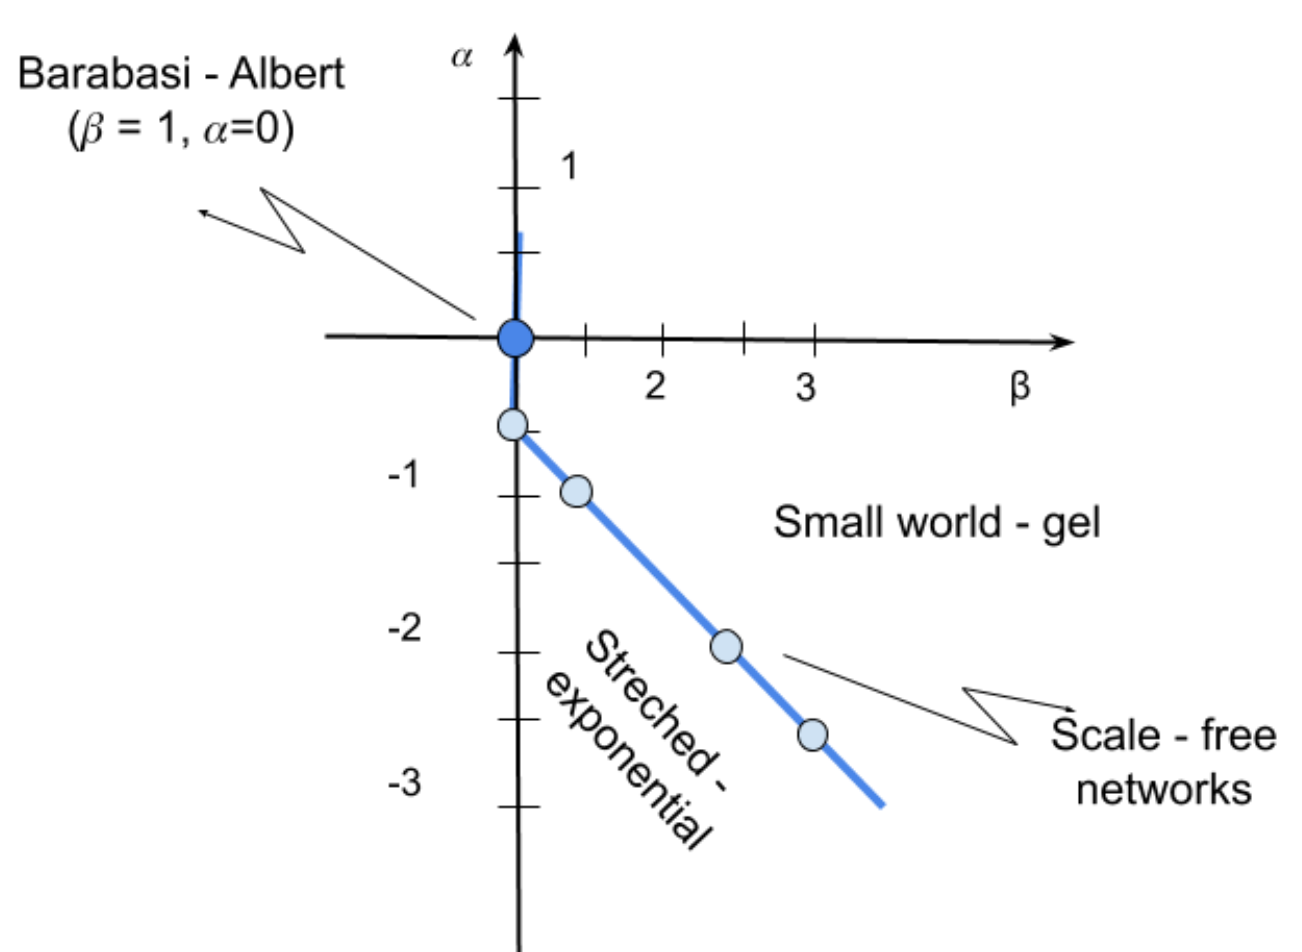
\includegraphics[width=0.5\linewidth]{Figures/diagram.png}
%	\caption{Phase diagram of aging network model}
%	\label{fig:diagram}
%\end{figure}


The networks generated with constant growth signal are uncorrelated trees. 

To enable formation of clusters in the network new nodes need to create more than one link. We adapt the original model such that at each time step we add $M\geq1$ new nodes that make $L\geq1$ links with existing nodes in the network corresponding to probability \ref{eq:1}. 
The master equation for $N_k$, $k$ degree nodes can be written as:

\begin{equation}
\partial_{t}N_{k}=\sum^{M(t)}_{j=1}r_{k-j\longrightarrow k}N_{k-j}-\sum^{M(t)}_{j=1}r_{k\longrightarrow k+j}N_{k}+M(t)\delta_{k,L} . \label{eq:aging_master}  
\end{equation}

At each time step we add $M(t)$ nodes with $L$ links. As multiply links between two nodes are not allowed, we'll get $M(t)$ new nodes with degree $L$, that describes third term in the equation. Old nodes can increase their degree from 1 to $M(t)$, as same node can be chosen by different new nodes. The first term in the equation describes nodes with degree $k\in\{k-M(t),\ldots, k-1\}$ that getting degree $k$, while in second term nodes with degree $k$ entering degree  $k\in\{k+1,\ldots, k+M(t)\}$. The quantities $r_{k-j\longrightarrow k}$ and $r_{k\longrightarrow k+j}$ are the rates that express the transitions of a node from class with degree $k-j$ to one with degree $k$ and from class with degree $k$ to class with degree $k+j$ respectively. 

The equation \ref{eq:aging_master} is not solvable in a general case. It was solved for the case $M(t)=1$ and specific values of parameters $\alpha$ and $\beta$ using continuous approach \cite{dorogovtsev2001b}. In this work, we use numerical simulations to explore the case when $M(t)$ is a correlated time-varying function and study how these properties influence the structure of generated networks for different values of parameter $-\infty<\alpha\leq-1$ and $\beta\geq1$ and constant $L$.


\section{Structural differences between networks }

%\subsection{D-measure}

%Between two nodes in the network, we can define different paths, but the most important one are the shortest paths, $d_{ij}$. Diameter defines the largest shortest path found in the network. For each node $i$ we can define the distribution of the shortest paths between node $i$ and all others nodes in the network, $P_{i}=\{p_{i}(j)\}$, where $p_{i}(j)$ is percent of nodes at distance $j$ from node $i$. The connectivity patterns can efficiently describe difference between two networks.    
%To specify how much $G$ and $G^{'}$ are similar we use D-measure \cite{tiago2}

%\begin{equation} 
%\label{eq:dmeasure}
%D(G,G') = \omega \left| \sqrt{\frac{J(P_1,..P_N)}{log(d)}}-\sqrt{\frac{J(P_1^{'},..P_N^{'})}{log(d^{'})}} \right| \nonumber +  (1-\omega) \sqrt{\frac{J(\mu_{G},\mu_{G^{'}})}{log2}}.
%\end{equation}

%D-measure calculates Jensen-Shannon divergence between $N$ shortest path distributions, $J(P_1,.., P_N)) = \sum_{i,j}p_i(j)log(\frac{p_i(j)}{\mu_j})$, where  $\mu_j = (\sum_{i=1}^N p_i(j))/N$ is mean shortest path distribution. The first term in equation \ref{eq:dmeasure} compares local differences between two networks, and Jensen-Shannon divergence between $N$ shortest path distributions $J(P_{1},...,P_{N})$ is normed with network diameter $d$. The second part determines global differences, computing  ${J(\mu_{G},\mu_{G^{'}})}$ between mean shortest path distributions. We consider equally important local and global properties of the networks, and parameter $\omega$ is set to $0.5$. The D-measure ranges from $0$ to $1$. The lower D-measure is, networks are more similar and for D-measure $D = 0$, structures are isomorphic.

The advantage this measure has is that it can distinguish between networks generated with the same model parameters. To examine how different growth signals influence the network structure, we use D-measure and compare networks generated with the same model parameters $\alpha$, $\beta$ and fixed number of links per new node $L$, but different growth signals. The growth of first network is driven by fluctuating signal $M_1 = {M(t)}$, while the other one grows by constant rate $M_2=<M(t)> = const$. 

We focus on the region of model phase diagram with negative $\alpha$ and positive $\beta$ as there is found the transition line from stretched-exponential across scale-free to the small world- gel networks. We take range of parameters  $-3\leq\alpha\leq-0.5$ and $1\leq\beta\leq3$ with steps $0.5$ and we also vary the the number of links each new node can create $L\in{1, 2, 3}$. For each combination of $(\alpha, \beta, L)$ we generate the sample of $100$ networks, and compare the structure of network grown with fluctuating and the constant signal. The results represented by D-measure are obtained averaging the D-measure between all possible pairs of generated networks.     

\begin{figure}[h!]
	\centering
	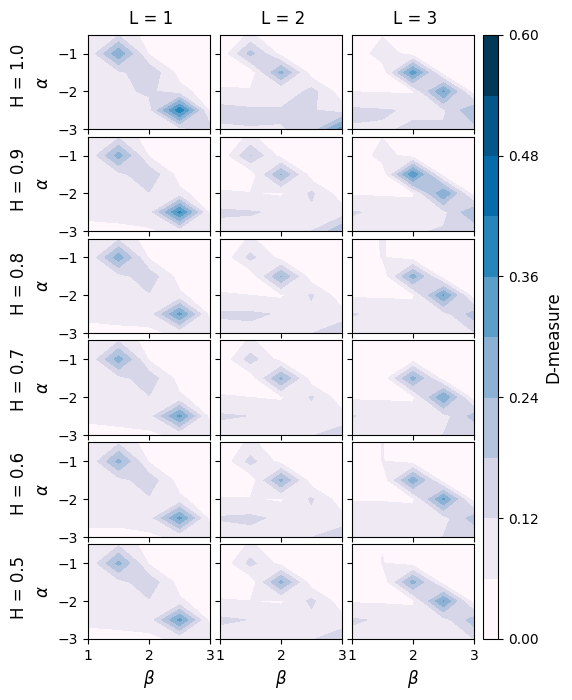
\includegraphics[width=0.5\textwidth]{Figures/Ddist_M4_w10.5_w20.5.png}
	\caption{D-distance between networks generated with different long-range correlated signals with fixed value of Hurst exponent and networks generated with constant signal M=4.}
	\label{fig:Ddist_m}
\end{figure}

First, we explore how monofractal signals, see Figure \ref{fig:monofractals} shape the structure of complex networks. The D-measure between networks grown with monofractal signal, with $H \in \{0.5, 0.6, 0.7, 0.8, 0.9, 1.0\}$ and constant signal $M=4$ are shown in figure \ref{fig:Ddist_m}. The higher values of D-measure are found in the region of critical line $\beta(\alpha^{*})$. The most considerable influence is on networks with scale-free distribution. Comparing D-distance in only one point of  phase diagram, for example $L=1, \alpha = -2.5, \beta = 2.5$, we find correlations in the signal (Hurst exponent is larger), make bigger impact on the network structure. D-measure between networks grown with signal with Hurst exponent $H=1.0$ and constant signal is $D(H=1.0, M=4) = 0.405$, while between networks grown with signal with $H=0.8$ and constant signal is $D(H=0.8, M=4) = 0.316$. For $\alpha>\alpha^{*}$ networks have similar structural properties and D-measure is close to 0. In the region of networks with stretched exponential degree distribution $\alpha<\alpha^{*}$  differences are small.  

For signals from real communities we find non-zero values of D-measure \ref{fig:dmeasure}. The largest difference between networks is as before along critical line $\beta(\alpha^{*})$, for scale free network. For values $\beta<\beta(\alpha^{*})$ the structural differences exist, but they become smaller. In the region of gel small world networks $\alpha>\alpha^{*}$ structural differences are small and close to zero. In the region around critical line we find that D-measure depends on the properties of the signal. Multifractal signals TECH has the largest impact on network structure; the maximum obtained value of D-measure is $D_{max}=0.552$. Similar behavior we discover for other multifractal signals, random TECH and MySpace. For networks generated with uncorelated signals, random mySpace and Poisson, difference exists but it is much smaller and comparable with monofractal signals.  


\begin{figure}[h!]
	\centering
	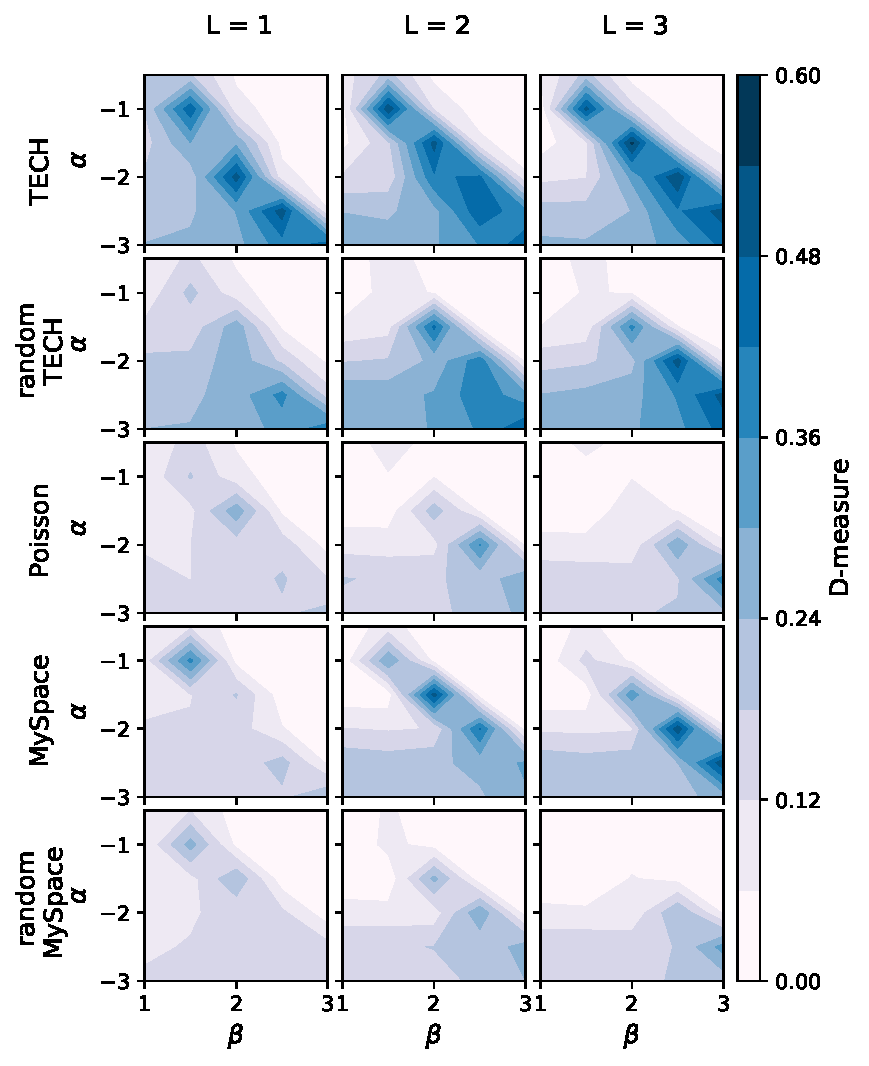
\includegraphics[width=0.5\linewidth]{Figures/Ddistance.pdf}
	\caption{The comparison of networks grown with growth signals shown in figure \ref{fig:signals} versus ones grown with constant signal $M=1$, for value of parameter $\alpha\in[-3,-1]$ and $\beta\in[1,3]$. $M(t)$ is the number of new nodes, and $L$ is the number of links added to the network in each time step. The compared networks are of the same size.}
	\label{fig:dmeasure}
\end{figure}

The position of the critical line slightly moves toward larger $\beta$ with higher link density $L$. The addition of more than one node does not influence its position. Although, for fixed network density, we find a critical line independent of the growth signal's properties as can be seen in Figures \ref{fig:dmeasure}, \ref{fig:Ddist_m}. 

We can note that D-measure rises for lower $\alpha$. In the case of constant signal, number of nodes added to the network is equal for each time step, so at time interval $T$ the network has $MT$ nodes. In fluctuating signal the number of nodes  added during time interval $T$ vary with time. In signals, such as TECH, where are present peaks in the number of new users, emergence of hubs happens faster. As we decrease the parameter $\alpha$, fluctuations present in the signal become more important and emergence of the hubs happens even for uncorrelated signals. The trends present in the real signals further promote the emergence of hubs in the network.    

\subsection{The assortativity and clustering}

We further explore the assortativity index and clustering coefficient of networks generated with monofractal signals with different values of Hurst exponent. We show results for several ageing model parameters to show the difference between network this model can produce, \ref{fig:aindex}. All networks are disassortative, with a negative degree-degree correlation index. For the values of parameters below critical line, $\alpha=-2.5, \beta=1.5$ $r$ does not depend on the Hurst exponent. Above the critical line are small-world networks, and they are disassortative with a minimum value of assortativity index $r =-1$, for $L=1$, indicating the presence of a hub that connects to many nodes. The assortativity index slightly grows with link density. 

In the region of critical parameters, the assortativity index depends on the value of the Hurst exponent. The larger influence on the assortativity index have correlated signals, with Hurst exponent $H>0.8$, so networks become more disassortative, see line for parameters $L=1, \alpha=-2.5, \beta=2.5$ in Figure \ref{fig:aindex}. The long-range correlations have a stronger effect on the evolution of networks with lower density. 

We calculate the mean clustering coefficient, Figure \ref{fig:aindex}. For $L=1$ networks are uncorrelated trees, with clustering coefficient $0$. For network density $L>1$, nodes are organized into clusters. Under the critical line, for parameter  $L=3, \alpha=-2.5, \beta=1.5 $, clustering coefficient is constant and low. Similar values are obtained for clustering coefficient for critical parameters $L=3, \alpha=-1.5, \beta=2.0$, but for Hurst exponent $H>0.8$ clustering coefficient increase. Small world networks,  $L=3, \alpha=-1.5, \beta=2.5$ are clustered, the value of $<c>$ is high.  The value of clustering for networks created with the constant signal is 0.8. Networks grown with white noise signal and signal with H=0.6 have higher values of the clustering, while networks grown with signals that have Hurst exponent larger than 0.6 have the same value of clustering, which is below 0.8. 
 
\begin{figure}[h!]
	\centering
	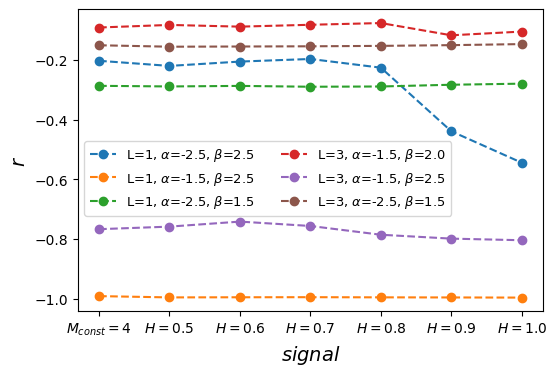
\includegraphics[width=0.45\textwidth]{Figures/aindex.png}
	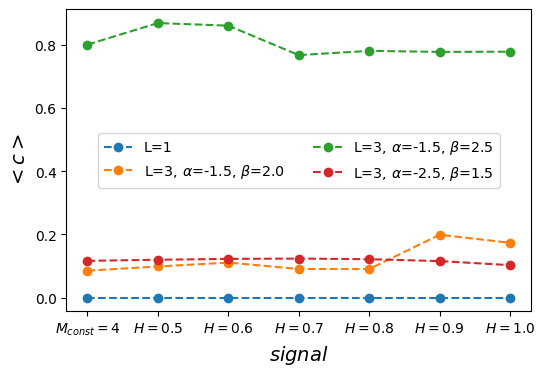
\includegraphics[width=0.45\textwidth]{Figures/clustering.png}
	\caption{Aindex}
	\label{fig:aindex}
\end{figure} 

We examine degree distribution, degree correlations and clustering coefficient of networks generated by real signals, as researchers has shown that these measures provide the sufficient set for discribing structure of complex network. D-measure showed that multifractals have larger influence on networks than monofractals, especially on scale-free networks. 

Figure \ref{fig:properties_sf} shows properties of networks generated with model parameters $L=2$, $\alpha=-1.0$, $\beta=1.5$, that lies on critical line.  The degree distributions $P(k)$ of networks generated with real signals TECH and MySpace have emergence of super-hubs. Degree distributions generated with randomized signals and white noise signal do not differ from degree distribution of networks generated with constant signal. Networks generated with real signals average neighbouring degree $\langle k\rangle_{nn}(k)$ and clustering coefficient $c(k)$ depend on node degree, while in networks generated with constant and randomized signals they weakly depend on the degree $k$.

\begin{figure}[h!]
	\centering
	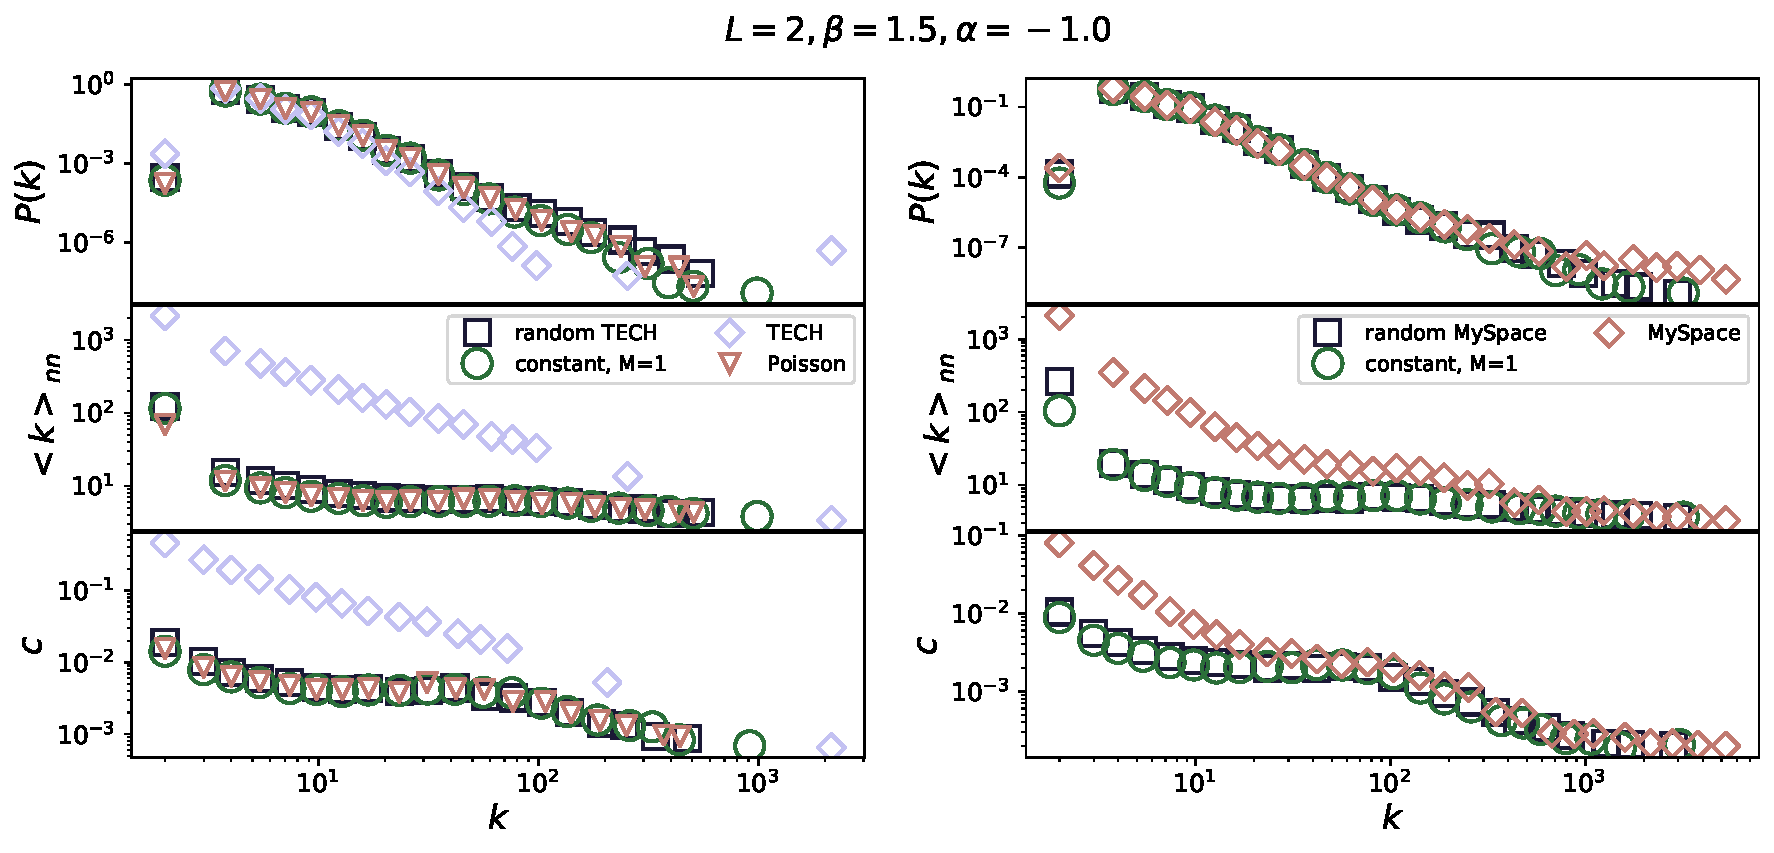
\includegraphics[width=0.7\textwidth]{Figures/b1.pdf}
	\caption{Degree distribution, the dependence of average first neighbor degree on node degree, dependence of node clustering on node degree for networks grown with different time-varying and constant signals. Model parameters have value $\alpha=-1.0$, $\beta=1.5$  and $L=2$ for all networks. The networks are from scale-free class.}
	\label{fig:properties_sf}
\end{figure}

We also find structural differences between networks, obtained with model parameters under the critical line $\alpha<\alpha^{*}$, see Figure \ref{fig:properties_se}. The difference is mostly found for TECH signal. Degree distribution $P(k)$ shows emergence of hubs in networks grown with TECH signal, while the randomized and Poisson signal are more similar to networks grown with constant signal. MySpace signal; whose generalized Hurst exponent $H(q)$ weakly depends on scale parameter $q$ and whose long-range correlations and trends are easily destroyed; do not influence the structure of networks more than constant or randomized signal.   

\begin{figure}[h!]
	\centering
	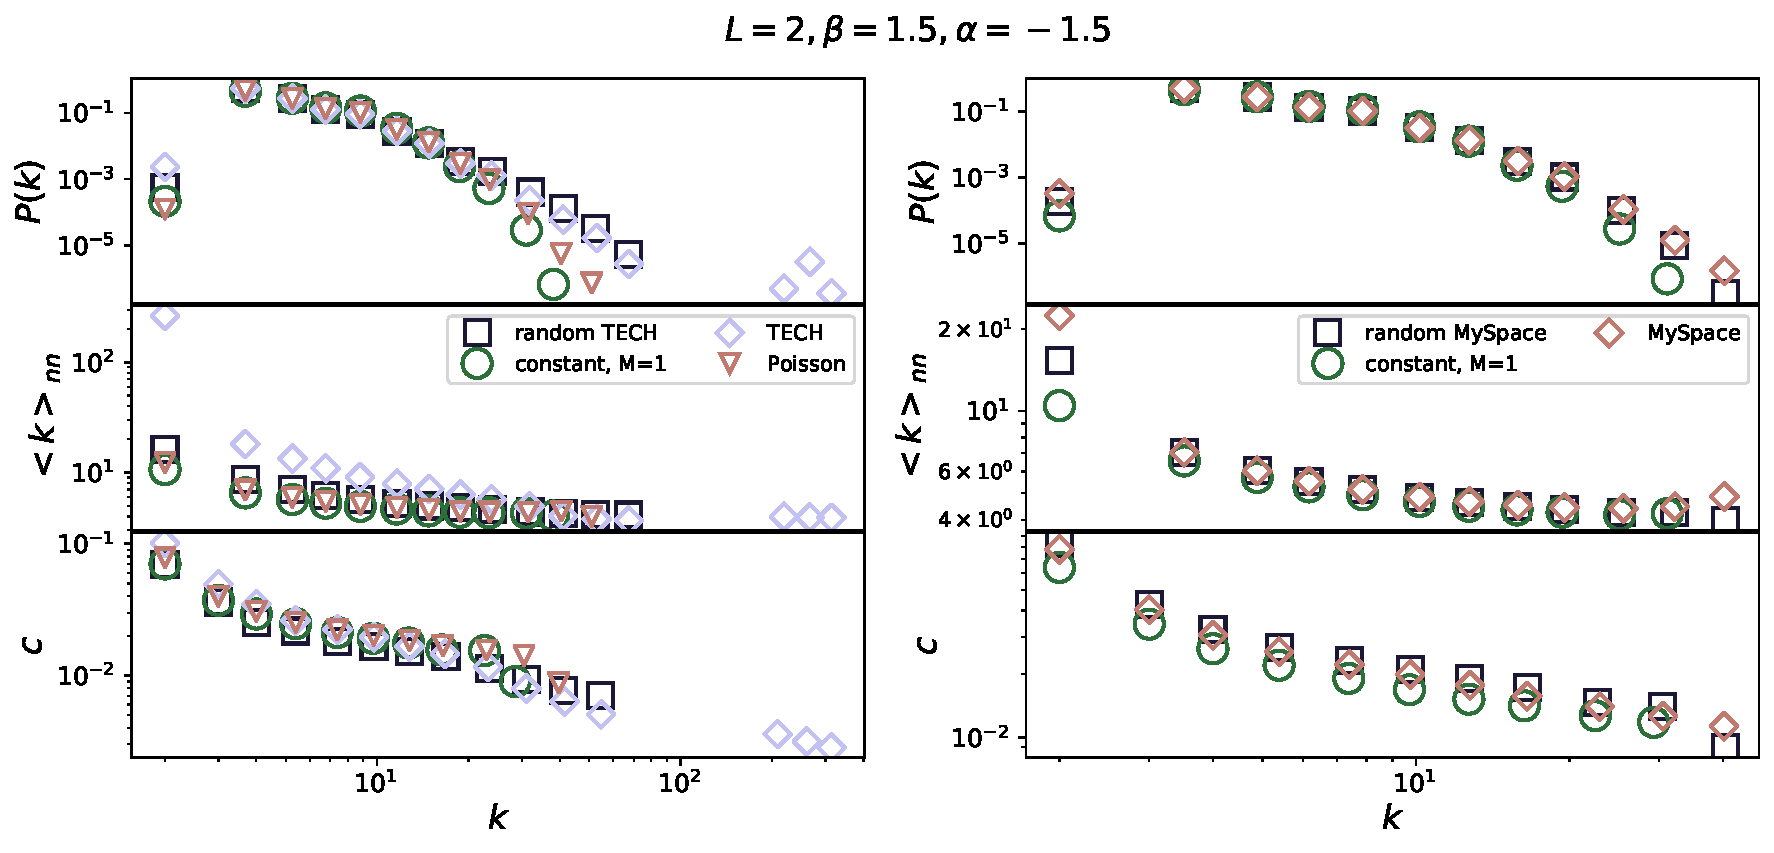
\includegraphics[width=0.7\textwidth]{Figures/b3.pdf}
	\caption{Degree distribution, the dependence of average first neighbor degree on node degree, dependence of node clustering on node degree for networks grown with different time-varying and constant signals. Model parameters have value $L=2, \alpha=-1.5$, $\beta=1.5$. The networks have stretched exponential degree distribution.}
	\label{fig:properties_se}
\end{figure}

The properties of time-varying signal do not influence the topological properties of small-world gel networks, Figure \ref{fig:properties_sw}. Here model promote existence of hubs. As this is mechanism through which the fluctuations alter the structure of evolving networks, the properties of the signal are not relevant.  


\begin{figure}[h!]
	\centering
	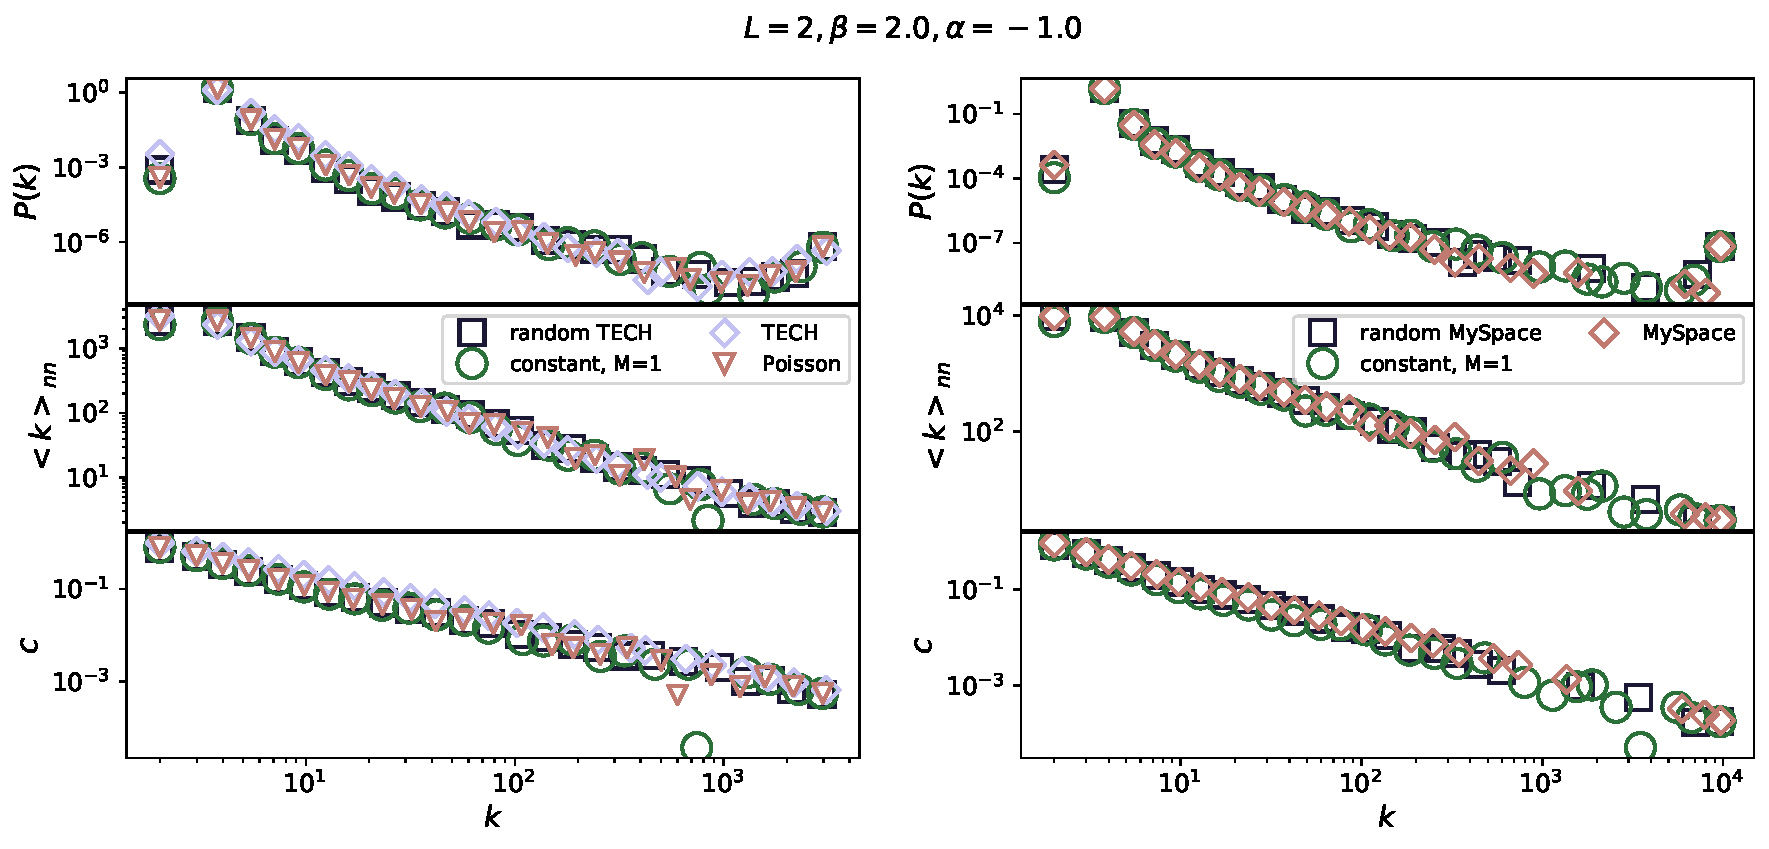
\includegraphics[width=0.7\textwidth]{Figures/b2.pdf}
	\caption{Degree distribution, the dependence of average first neighbor degree on node degree, dependence of node clustering on node degree for networks grown with different time-varying and constant signals. Model parameters have value $ L=2, \alpha=-1.0$, $\beta=2.0$. Generated networks have scale-free properties.}
	\label{fig:properties_sw}
\end{figure}


\newpage 
\section{Conclusions}

We demonstrate that the resulting networks' structure depends on the features of the time-varying signal that drives their growth. The previous research \cite{mitrovic2012,mitrovic2015} indicated the possible influence of temporal fluctuations on network properties. Our results show that the temporal properties of growth signals generate networks with power-law degree distribution, non-trivial degree-degree correlations, and clustering coefficient even though the local linking rules, combined with constant growth, produce uncorrelated networks for the same values of model parameters \cite{hajra2004}. 

We observe the most substantial dissimilarity in network structure along the critical line, the values of model parameters for which we generate networks with broad degree distribution. Figure \ref{fig:dmeasure} shows that dissimilarity between networks grown with time-varying signals and ones grown with constant signals always exists along this line regardless of the features of growth signal. However, the magnitude of this dissimilarity strongly depends on these features. We observe the largest structural difference between networks grown with multifractal TECH signal and networks that evolve by adding one node in each time step. The identified value of D-measure is similar to one calculated in the comparison between sub-critical and super-critical Erd\"{o}s–R\'{e}nyi graphs \cite{tiago2} indicating the considerable structural difference between these networks. Our findings are further confirmed in figure \ref{fig:properties}(b). The networks generated with signals that have trends and long-range temporal correlations differ the most from those grown with the constant signal. Our results show that even white-noise type signals can generate networks significantly different from ones created with constant signal for low values of $\alpha^{*}$.

The value of D-measure declines fast as we move away from the critical line, figure \ref{fig:dmeasure}. The main mechanism through which the fluctuations influence the structure of evolved networks is the emergence of hubs and super hubs. For values of $\alpha<<\alpha^{*}$, the nodes attache to their immediate predecessors creating regular networks without hubs. For $\alpha \sim \alpha^{*}$ graphs have stretched exponential degree distribution with low potential for the emergence of hubs. Still, multifractal signal TECH enables the emergence of hub even for the values of parameters for which we observe networks with stretched-exponential degree distribution in the case of constant growth figure \ref{fig:properties}(a). By definition, small-world gels generated for $\alpha>\alpha^{*}$ have super-hubs \cite{hajra2004} regardless of the growth signal, and therefore the effects that fluctuations produce in the growth of networks do not come to the fore for values of model parameters in this region of $\alpha-\beta$ plane.

Evolving network models are an essential tool for understanding the evolution of social, biological, and technological networks and mechanisms that drive it \cite{boccaletti2006}. The most common assumption is that these networks evolve by adding a fixed number of nodes in each time step \cite{boccaletti2006}. So far, the focus on developing growing network models was on linking rules and how different rules lead to networks of various structural properties \cite{boccaletti2006}. Growth signals of real systems are not constant \cite{mitrovic2015,mitrovic2012}. They are multifractal, characterised with long-range correlations \cite{mitrovic2015}, trends and cycles \cite{suvakov2013}. Research on temporal networks has shown that temporal properties of edge activation in networks and their properties can affect the dynamics of the complex system \cite{holme2012}. Our results imply that modeling of social and technological networks should also include non-constant growth and that its combination with local linking rules can significantly alter the structure of generated networks.

%----------------------------------------------------------------------------------------




% Chapter 1

\chapter{Groups growth model} % Main chapter title

\section{Introduction}

Social groups, informal or formal, are building mesoscopic elements of every socio-economic system. Their emergence, evolution, and disappearance are at the heart of change in a social system \cite{}. Settlements, villages, towns and cities are formal and highly structured social groups of countries. Their organisation and growth determine the functioning and sustainability of every society \cite{barthelemy2016structure}. Companies are the building blocks of every economy and their dynamics are important indicators of level of development of every economy \cite{hidalgo2009building}. Scientific conferences, as a scientific groups, enable fast dissemination of the latest results, exchange and evaluation of ideas as well as a knowledge extension, and thus are integral part of science \cite{smiljanic2016theoretical}. The membership of individuals in various social groups, online and offline, can be essential when it comes to quality of their life \cite{montazeri2001anxiety, davison2000talks, cho2012tea}. Therefore, it is not surprising that the social group dynamics and their sustainability are at the center of the attention of many researchers \cite{aral2012identifying,gonzalez2013broadcasters, torok2013opinions, yasseri2012dynamics}.\\

The abundance of data enabled the application of methods and paradigms from statistical physics in studying the structure and dynamics of social systems \cite{castellano2009statistical}. The main argument for using statistical physics to study social systems is that they consist of a large number of interacting individuals. Due to this, they exhibit different patterns in their structure and dynamics, commonly known as \textit{collective behavior}. A collective behavior, observed both in physical and social systems, is enforced by a few basic properties of building units and is independent of all other characteristics. The phenomenon is known as \textit{universality} in physics and is commonly observed in social systems such as in voting behavior \cite{chatterjee2013universality}, or scientific citations \cite{radicchi2008universality}. The discovery of universality and scaling in phenomena indicate the existence of universal and straightforward mechanisms that govern the dynamics of a system \cite{}.\\  


The availability of large-scale and long-term data on various online social groups has enabled the detailed empirical study of their dynamics. The focus was mainly on the individual groups and how structural features of social interaction influence whether individuals will join the group \cite{backstrom2006group} and remain its active members \cite{smiljanic2016theoretical, smiljanic2017associative}. The study on LiveJournal \cite{backstrom2006group} groups has shown that decision of an individual to join a social group is greatly influenced by the number of her friends in the group and the structure of their interactions. The conference attendance of scientists is mainly influenced by their connections with other scientists and their sense of belonging \cite{smiljanic2016theoretical}. The sense of belonging of an individual in social groups is achieved through two main mechanisms \cite{smiljanic2017associative}: expanding of the social circle at the beginning of joining the group and strengthening of the existing connections in the later phase. The dynamics of social groups depend on their size \cite{}. Analysis of the evolution of large-scale social networks has shown that edge locality plays a critical role in the evolution of social networks \cite{leskovec2008microscopic}. Small groups are more cohesive with constant membership, while large groups tend to change their active members constantly \cite{PNAS}. Previous research focused on the growth of the single group, the evolution of its social network, and the influence of the structure on its growth. However, how growth mechanisms influence the distribution of members of one social system among groups is still anecdotal.\\

Furthermore, it is not clear whether the growth mechanisms of social groups are universal or system-specific. The size distribution of social groups has not been studied in great detail. Rare empirical evidence of size distribution of groups and communities indicates that it follows power-law behavior \cite{}.  The distribution of the size of the cities and firms has been studied in great detail. Analysis of the sizes of the cities shows that the distribution of all cities follows a log-normal distribution, while the distribution of the largest cities resembles Zipf's distribution \cite{fazio2015pareto}. The scaling behavior was observed in the growth of the companies \cite{stanley1996scaling}, while empirical evidence shows that distribution of company sizes follows log-normal behavior and remains stable over decades \cite{amaral1997scaling}. 

Can we create a unique yet relatively simple microscopic model that will reproduce the distribution of members between groups and explain the differences observed between social systems? French economist Gibrat proposed a simple growth model to reproduce companies' and cities' observed log-normal size distribution. However, the analysis of the growth rate of the companies \cite{amaral1997scaling} has shown that growth mechanisms are different from ones assumed by Gibrat. Analysis of the growth of three online social networks showed that population growth is not determined by the population size and spatial factors, and it deviates from Gibrat's law \cite{zhu2014online}. The growth through diffusion and growth by other means have been used as mechanisms in the model used for prediction of rapid group growth \cite{kairam2012life}. The growth mechanisms of various social groups and the source of the scaling observed in socio-economic systems thus remain hidden.\\

Here we analyze the distribution of formal social groups in two different systems: Meetup online platform and subreddits in the Reddit community. We analyze the scaling behavior of size distributions and distribution of growth rates. Analysis of the dependence of growth rates indicates that growth can not be explained through Gibrat's model. We propose a simple microscopic model that incorporates some of the results of previous research \cite{backstrom2006group}. In our model, the social system grows by adding a constant number of new individuals. The number of groups grows as well, and they overlap in terms of membership, i.e., one individual may be a member of more than one group. An individual can create a new group or join an existing one according to some probability. The choice of the existing group depends on the number of social connections already present. We show that the model can reproduce size distributions and growth rate distribution for both studied systems. We analyze the model and show that it can produce a broad set of distributions depending on the value of model parameters.\\

The paper is organized as follows: in Section \ref{sec:data} we describe the data, while in Section \ref{sec:emp} we present our empirical results. In Section \ref{sec:model} we introduce model parameter and rules. Section \ref{sec:results} we demonstrate that model can reproduce the growth of social groups in both systems and show the results for different values of model parameters. Finally, in Section \ref{sec:con}, we present concluding remarks and discuss our results. 


\section{Data \label{sec:data}}
We analyse the growth of social groups from two widely used online platforms: Reddit and Meetup. Reddit \footnote{https://www.reddit.com/} enables sharing diverse web content, while Meetup \cite{www.meetup.com} allows people to use online tools to organize offline meetings. Reddit users interact exclusively online through posts and comments. The building elements of the Meetup community are topic-focused groups, such as food lovers or ICT and data science professionals. Due to their specific activity patterns - events where members meet face-to-face - Meetup groups are geographically localised. 

We compiled the Reddit data from https://pushshift.io/. This site collects data daily and, for each month, publishes merged comments and submissions in the form of JSON files. 
Specifically, we focus on subreddits - social groups of Reddit members interested in a specific topic. We select all subreddits active in 2012 and follow their growth from their beginning until 2017. The considered dataset contains 17000 subreddits, with the oldest originating from 2003 and the youngest being from 2017.\\
For each post under a subreddit, we extracted the information about the user-id of the post owner, subreddit-id, and timestamp. We observed the data from $2006$ to the $2017$ year, and for each subreddit and user-id, we selected timestamp when a user made a post for the first time. For our analysis, we chose subreddits still active in $2017$ while removing small subreddits active for less than a month. The resulting dataset contains $304 007$ subreddits and  $36 595 134$ users. \\
For simulation, we extracted data until $2011-12$ and removed all subreddits with a small amount of activity. This reduced the dataset significantly - we obtained only $17 073$ subreddits with $2 195 677$ active users. 

The Meetup data were downloaded in $2018$ using public API. The Meetup platform was launched in 2003, and at the moment we accessed the data, there were more than 240000 active groups. For each group, we extracted information about the date it had been founded, its location, and the total number of members. We focused on the groups founded from $2003$ until $2017$ in big cities such as London and New York, where Meetup platform achieved considerable popularity. We considered groups active at least one month. There were 4673 groups with $831685$ members in London and 4752 groups with $1059632$ members in New York. In addition, we extracted the Id of each member in the group, which allowed us to obtain complementary information about the date a member joined a group. 

From collected data, for each group, we can calculate the number of new members per month and so the group sizes $S_i$ at each time step (month). The growth rate $R_i$ at step $i$ is obtained as logarithm of successive sizes $R = log(S_t/S_{t-1})$. 

%We select two locations, London and New York, and study the formation and growth of groups in these two locations from 2003 until 2017. The total number of groups studied for London is 4000 and 8000 for New York. 
%Potreban je slican opis za Meetup podatke

While these two communities differ in means of communication between their users and activities these users engage in, there are certain common properties that enable us to use same methods to study the growth of these groups and make comparative analysis of their growth. In both communities, users can create new groups and join existing ones. One user can be a member of more than one group/subreddit and there are no limits in the number of groups. For each meetup group we have an information on when an user has joined the group, i.e., we have an information about the group size at every moments. For a subreddit we have a detailed information about users' activity and this we have an information when a user made a first post. This moment is considered as the moment when the user has joined the subreddit and became an active member. In our case we do not consider activity of when a user leaves the group of subreddit, since this kind of information is not available to us. For these reasons, the size of groups we are considering is non-decreasing function. 

\section{Empirical analysis of social group growth \label{sec:emp}}
\begin{figure}[h!]
	\centering
	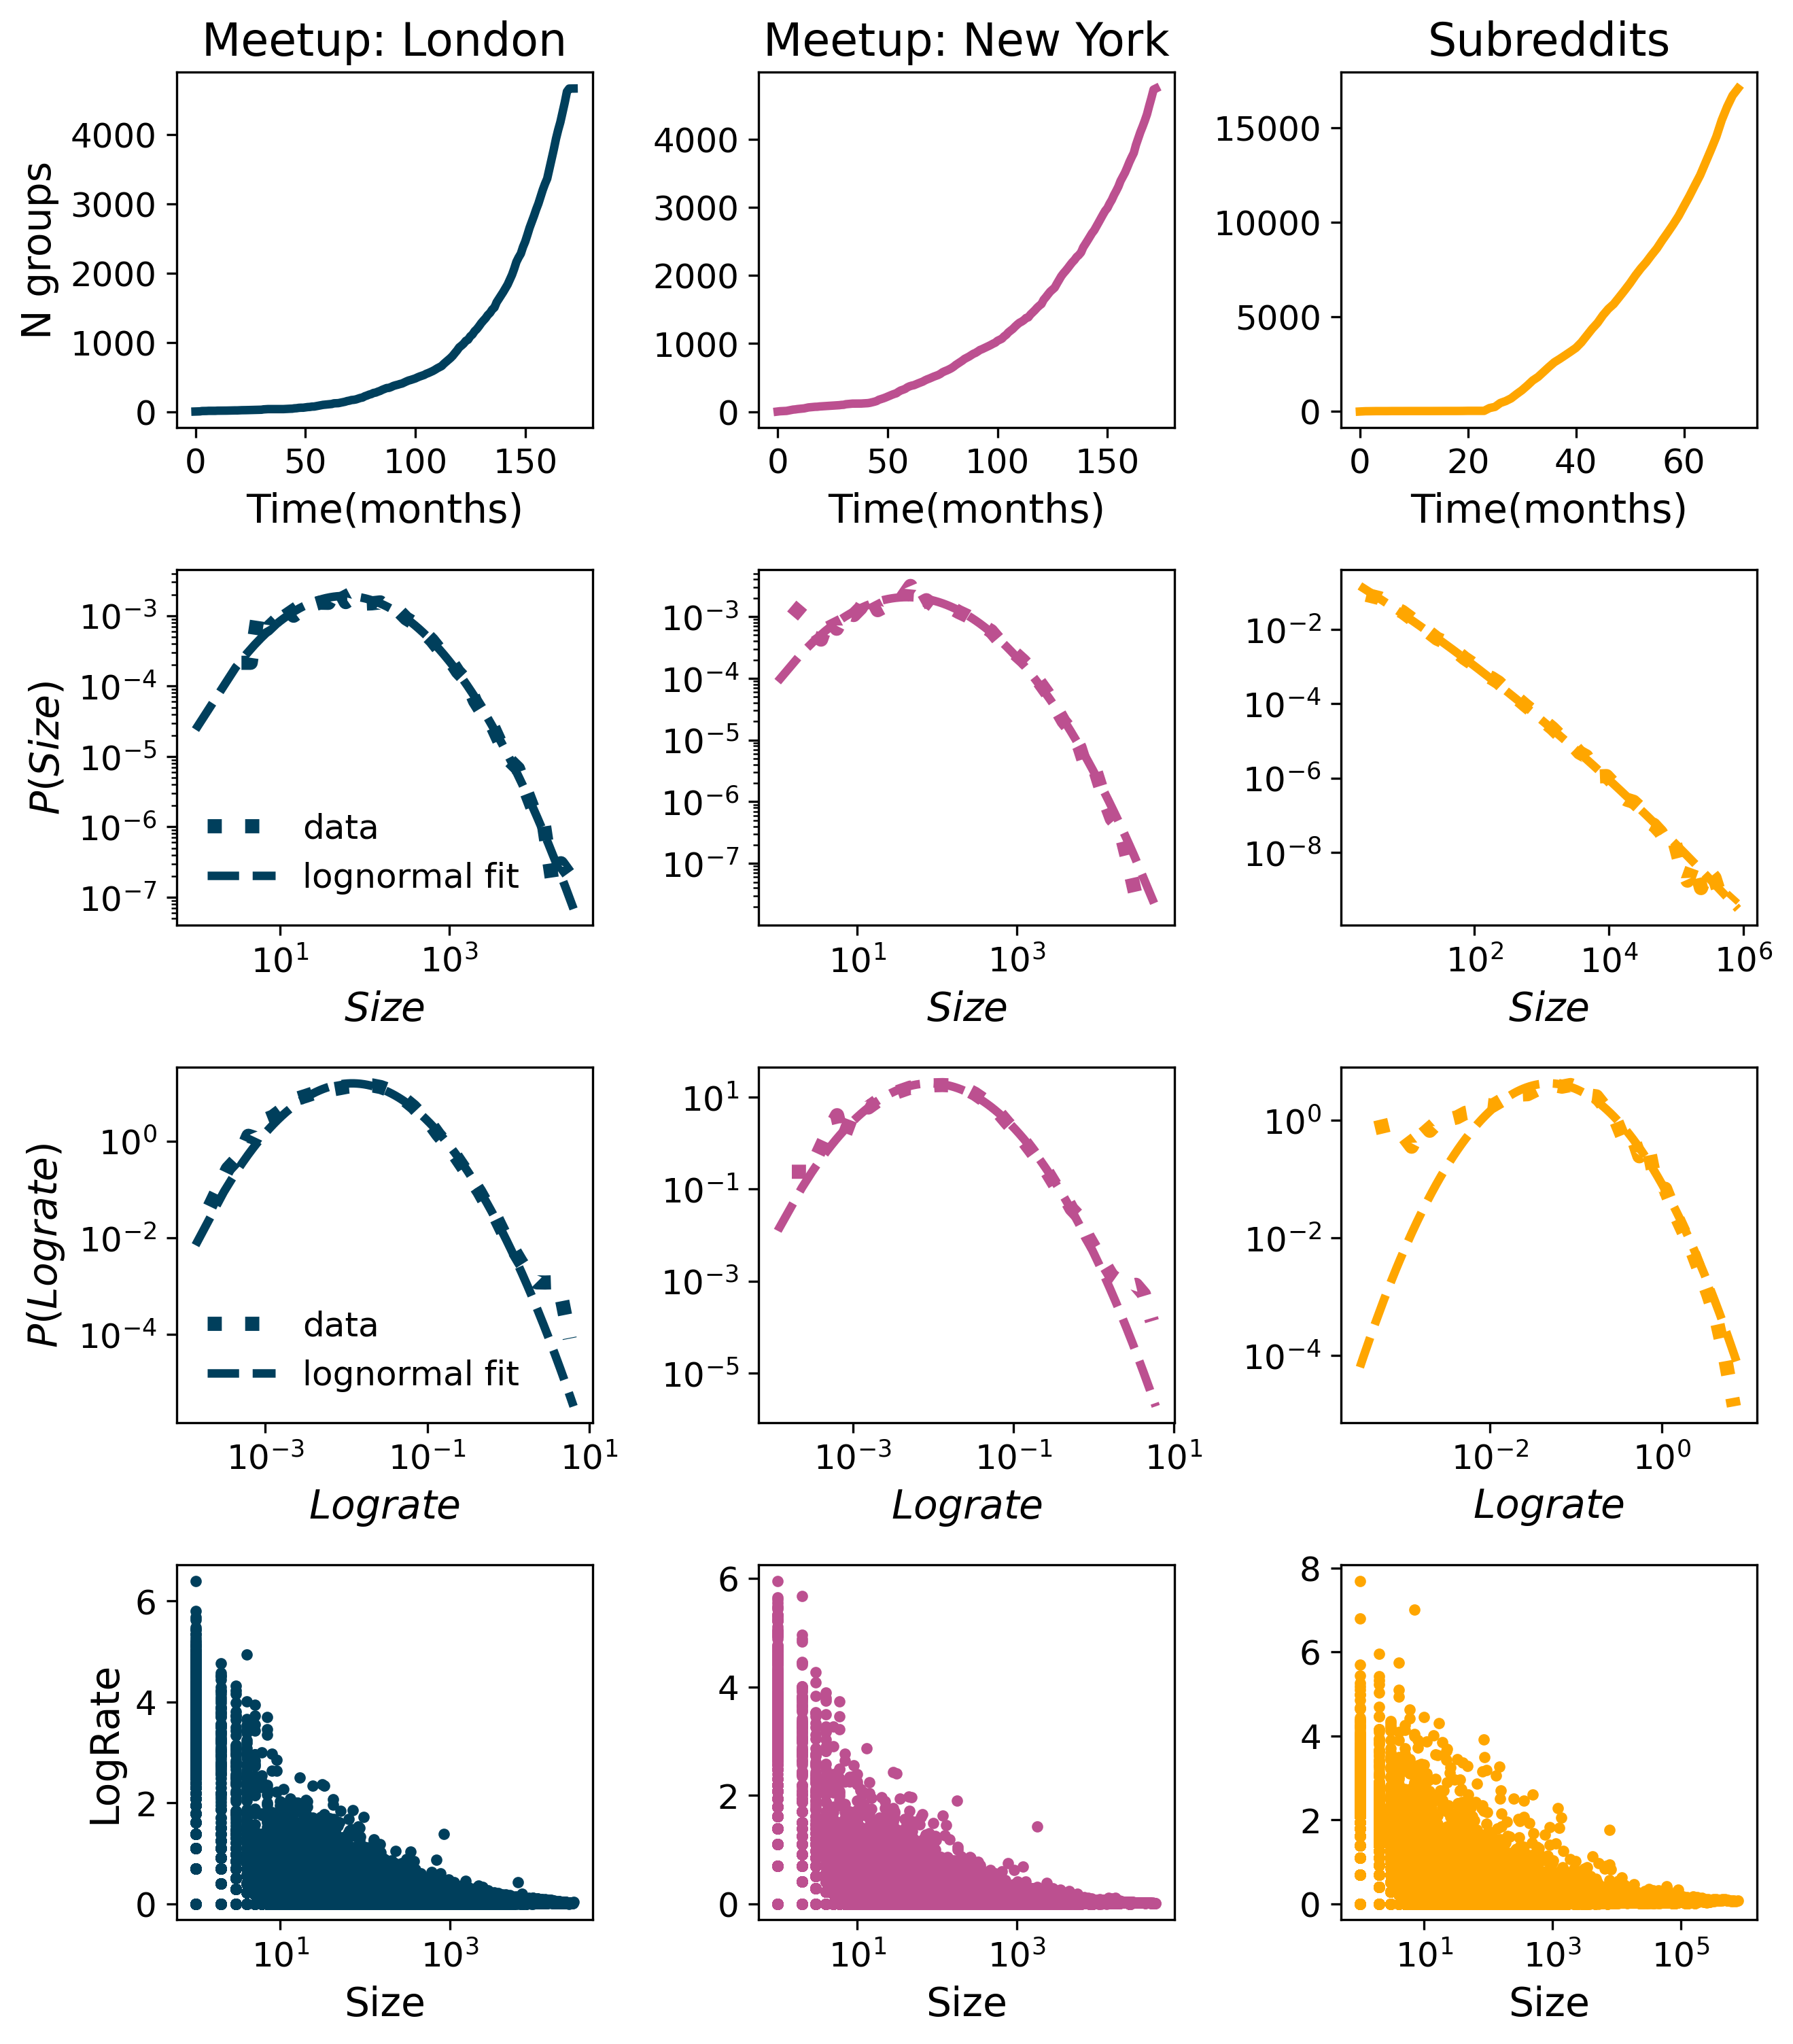
\includegraphics[width=0.6\linewidth]{Figures/Fig2.png}
	\caption{The number of groups over time, sizes distribution and logrates distribution for Meetup groups created in London from 08-2002 until 07-2017 that were active in 2017 and subreddits created in the period from 01-2006 to the  12-2011 that were active in 2017. }
	\label{fig:data1}
\end{figure}

Figure \ref{fig:data1} summarize properties of the groups in Meetup and Reddit networks. The number of groups grows exponentially over time. Nevertheless, we notice that Reddit has much more groups than Meetup and that Reddit groups are prone to engage more members in a shorter period of time (sizes of meetups range up to  $10^4$, while sizes of subreddits are up to $10^6$). The distributions of group sizes follows the lognormal distribution
\begin{equation}
P(S)=\frac{1}{S\sigma\sqrt{2\pi}}exp(-\frac{(\ln(S)-\mu)^{2}}{2\sigma^{2}})
\label{eq:log} \ ,
\end{equation}
where $S$ is the group size and $\mu$ and $\sigma$ are parameters of the distribution. We used package \cite{powerlaw} to fit Eq. \ref{eq:log} to Reddit and Meetup data and found that distribution of groups sizes for Meetup groups in London and New York follow the same distribution with the value of parameters $\mu= 5.96$, $\sigma = 1.38$. The distribution of sizes of subreddits also has the log-normal shape with parameters $\mu= -1.59$ and $\sigma = 3.99$. Even though these distributions are from the same class, for subreddits we find broader distribution that may resembl power-law distribution. Our strict analysis shown in Supportive Information (SI) confirms that the distribution exhibits a log-normal behavior.  

The lognormal distributions can be generated by multiplicative processes \cite{mitzenmacher2004brief}. If there is a quantity with size $S_i$ at time step $t$, it will grow so after time period $\delta$ the size of the quantity is $S(t+\Delta t) = S(t) r$, where $r$ represents a random process. The Gibrat law states that growth rates $r$ are uncorrelated and do not depend on the current size. In order to describe the growth of social groups, we calculate the logarithmic growth rates defined as $R = log\frac{S_t}{S_{t-\Delta t}}$. According to Gibrat law, the distribution of sizes follow lognormal distribution. For logarithmic growth rates expected distribution is normal, or as it is shown in many studies it is better explained with Laplacian (“tent  shaped“) distribution \cite{mondani2014fat}, \cite{fu2005growth}. In figure \ref{fig:data1} we calculate distributions of logrates for a time period of $\Delta=1 month$. For both networks Meetup and Reddit, logrates are very well approximated with lognormal distribution. The Fig. \ref{fig:data1} shows that logrates depen in the groups size, especially for the smaller and medium size groups. Our analysis of growth of social groups shows that this growth violates the basic assumptions of the Gibrat's law \cite{frasco2014spatially, qian2014origin}, and thus the this growth can not be explained as a simple multiplicative process.\\

We are considering a relatively large time period for online groups. The fast expansion of ICTs led to change of how users how users access online communities. With the use of smartphones the online communities became more available and which led to exponential growth of communities \ref{fig:fig4} and potential change in the mechanisms that influence growth of social groups in these communities. For these reasons we have aggregate groups according to year they were founded for each of the three datasets. For each year and each of the three datasets we calculate the average size of the group $<S>^{y}_{x}$, here $y$ is year and $x$ is the $L$, $NY$ or $R$ depending on the dataset, and normalize the size of the groups. The distribution of normalized sizes is shown in \ref{fig:scale}. All distributions exhibit log-normal behavior. Furthermore, the distributions for the same dataset and different years follow a universal curve with same value of parameters $\mu$ and $\sigma$. The universal behavior is observed for distribution of normalized logrates, shown in Fig. \ref{fig:scale} (bottom panel). This indicates that growth of the social groups did not change due to increased growth of users in online communities, but rather it indicates that the growth is independent on the size of the whole of the system.   

\begin{figure}[!h]
	\centering
	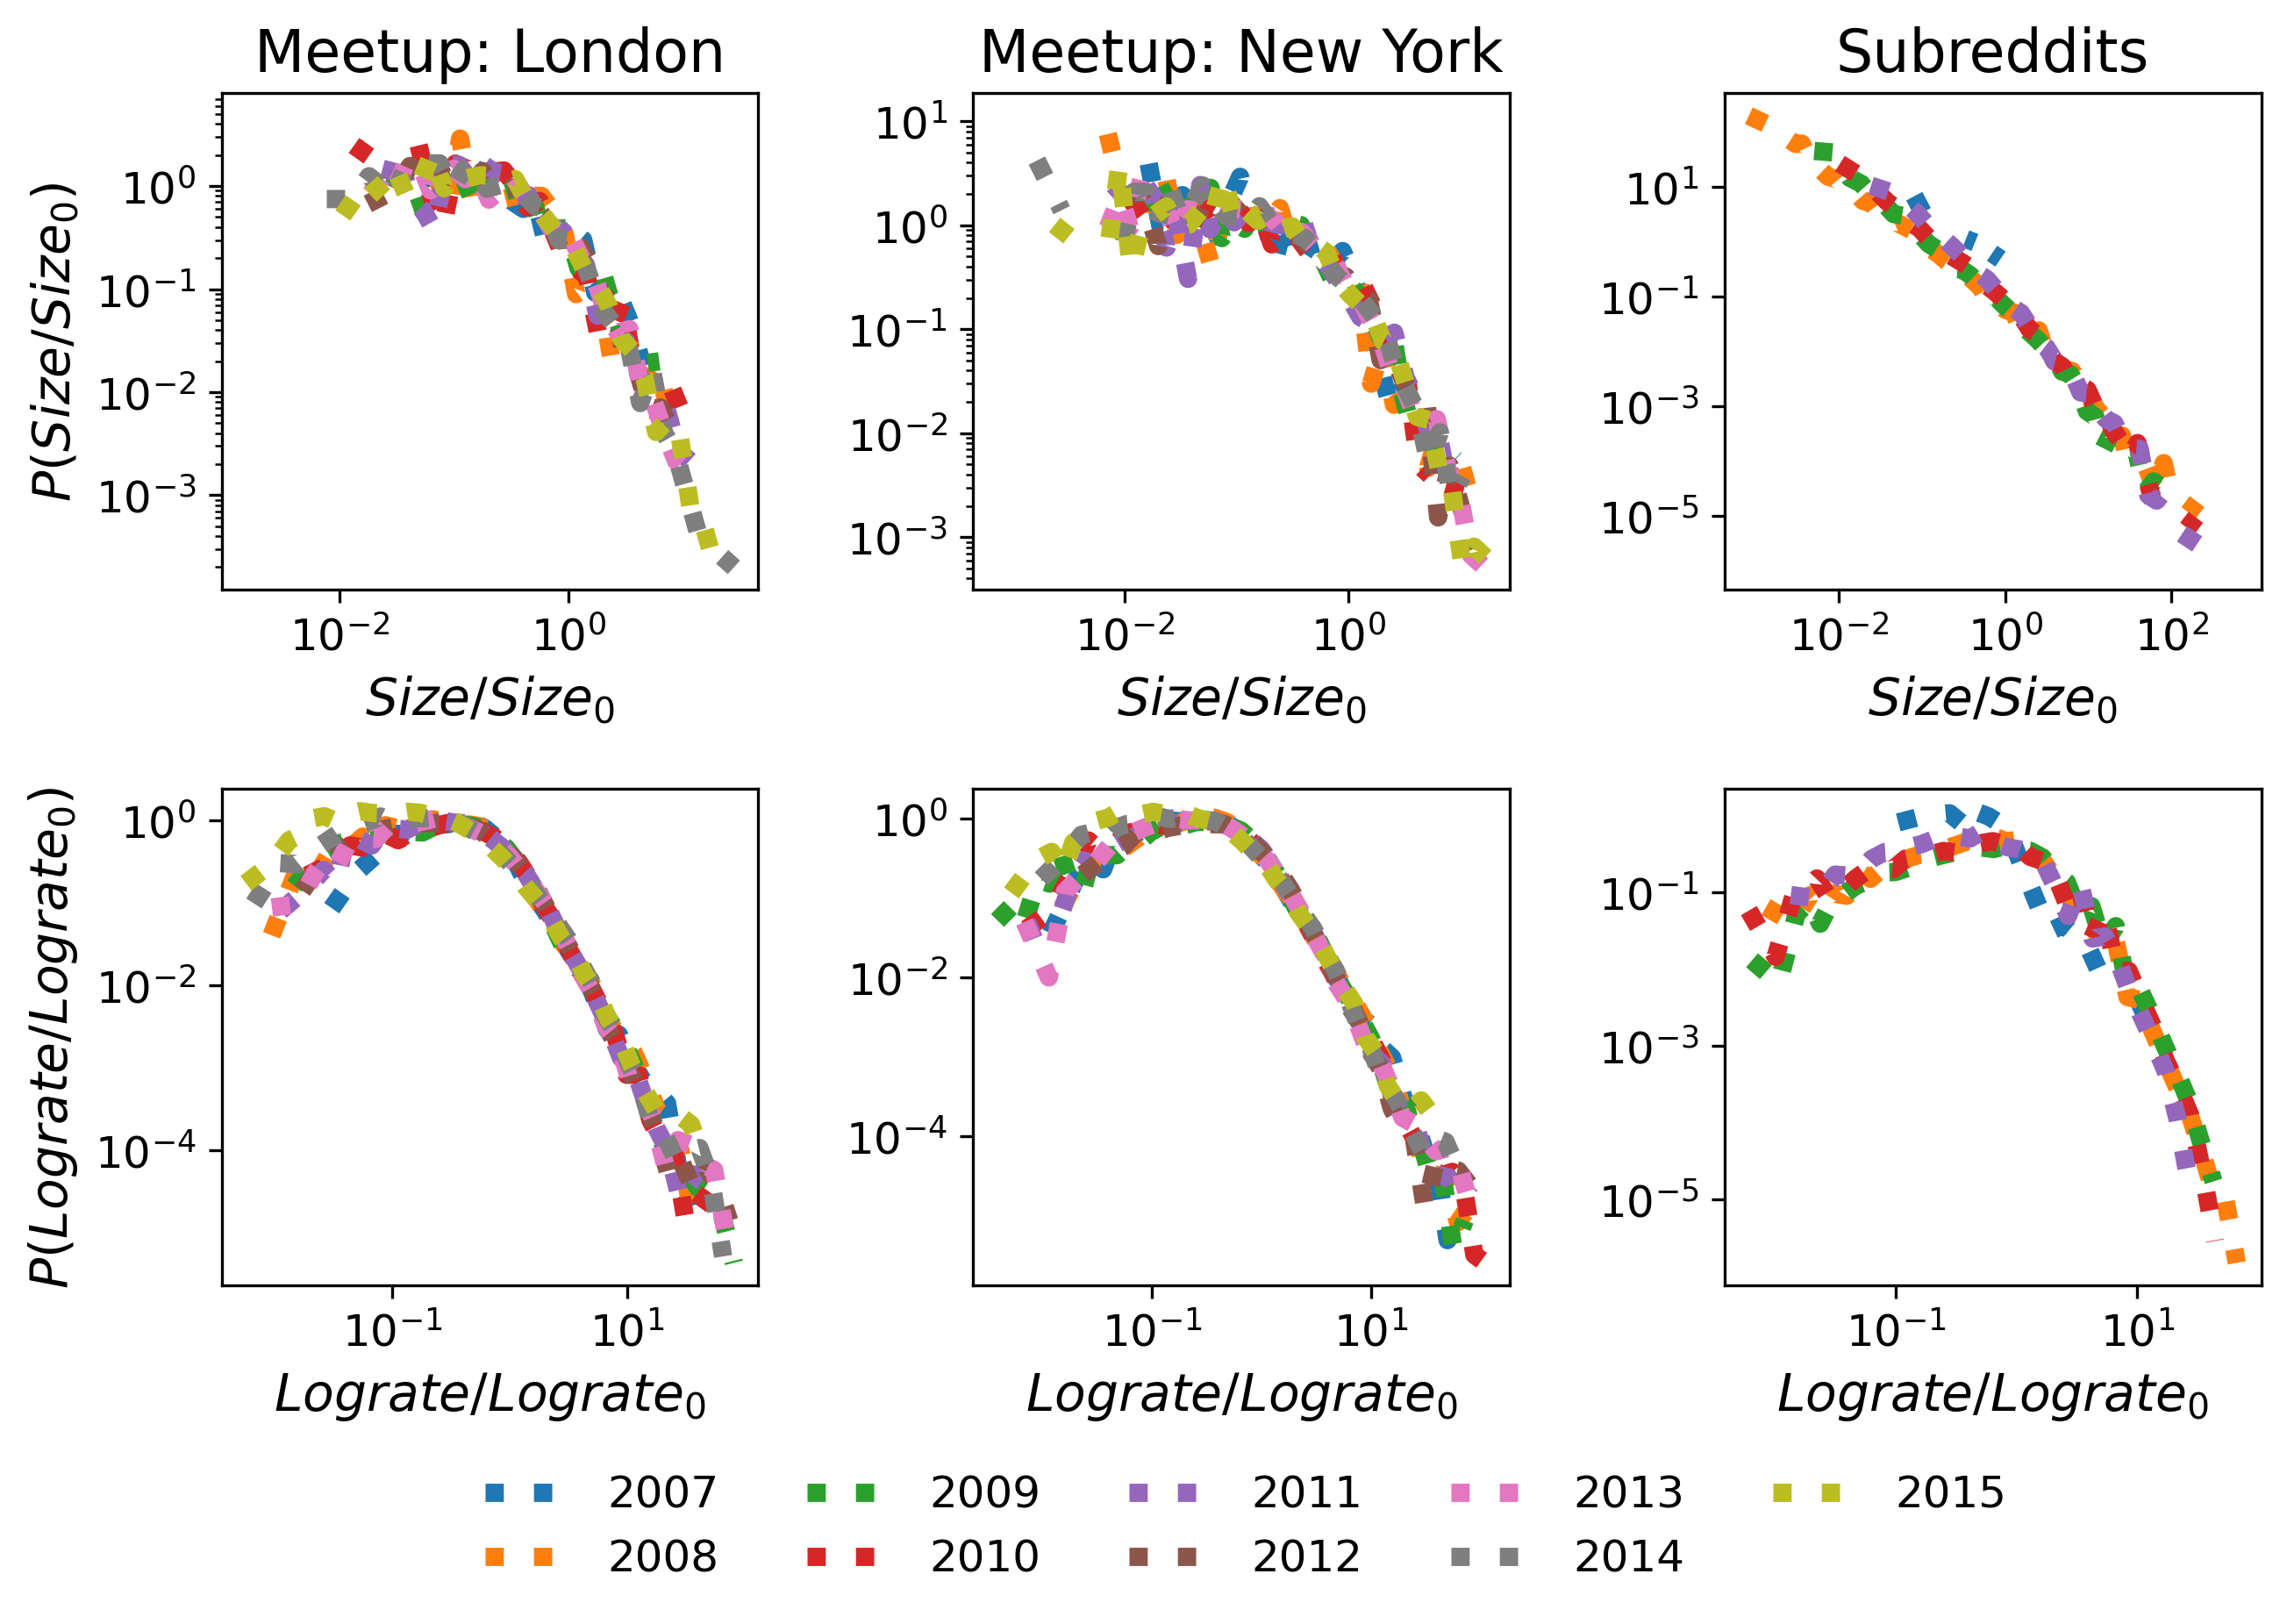
\includegraphics[width=0.8\linewidth]{Figures/Fig1.png}
	\caption{The figure shows the groups' sizes distributions and log rates distributions. Each distribution collects groups founded in the same year and is normalized with its mean value. The group sizes are at the end of 2017. for meetups and 2011. for subreddits. }
	\label{fig:scale}
\end{figure}

\section{Model \label{sec:model}}
Growth of social groups can not be explained with the simple rules of Gibrats law. Previous research on group growth and longevity has shown that social connections with members of a group influence individual's choice to join that group \cite{kairam2012life, zheleva2009co}. However, not only social connections, but also individual's interests and need to discover new content or activity may have an influence on individuals' diffusion between groups. Furthermore, social systems constantly grow since new members join every minute. The growth influences both dynamics of the system \cite{mitrovic2011quantitative, dankulov2015dynamics} and the structure of social interactions \cite{vranic2021growth}. Social groups are constantly created, allowing members to group around common interest or to further solidify their interactions through common activities. Based on these observations, we propose a model of group growth that combines these processes, see in Fig. \ref{fig:fig3}.\\

In our model, we represent a social system as a bipartite network, with two partitions of nodes, users and social group. By definition, the links in bipartite networks exist only between nodes belonging to two different partitions. In our model, the link indicates that the user is a member of a group. Previous studies have used a bipartite growing network model to describe the structure of the social network and its communities \cite{zheleva2009co, leskovec2008microscopic, yang2014structure, ZHANG20136100}. This representation of social system is especially useful in studying overlapping communities, where users can be members of multiple groups. The paper \cite{zheleva2009co} proposed a growing network model where a bipartite (referred to as affiliation) network interacts with the social network, such that users have a preference to the friend’s groups. In our data, we do not have information about explicit friendships. Yet to include diffusion growth of the social networks we assume that a new member links to a small number of individuals already present the in group.

In our model, we allow the growth of both network partitions, figure \ref{fig:my_label}. The partition of users grows through the addition of new users. The groups partition grows through creation of a new group and depends on users' activity. Before joining a group new user makes the link to a randomly chosen node in the social network. This condition allows each user to perform diffusion linking \cite{kairam2012life}. 

At each time step, we add $N_{u}$ new users. Old users are not active in each time step, but we control their activity with parameter $p_{a}$. Active users, new users and a sample of old users that were activate, have an option to create a new group with probability $p_{g}$ or to join one of the existing groups with probability $1-p_{g}$. If a user decides to join an old group, he/she chose with probability $p_{aff}$ to join the social group that is already populated by their friends. That group is chosen according to overlap of friendship connections. This way we mimic social diffusion process. With probability $1-p_{aff}$ a user can join randomly selected group. Through this step we mimic a behavior of users when they prefer to explore their interests or discover a new content or activity. 

Our model is different from one proposed in Ref. \cite{zheleva2009co}. In Ref. \cite{zheleva2009co} when user chooses with probability $p_{aff}$ the group of her friends, that group is chosen randomly from this list. When user decides to chose a group randomly, with probability $1-p_{aff}$, she selects a random group with probability proportional to its size. 
Combination of Preferential attachment leads to power-law shape of the distribution of group sizes \cite{zheleva2009co}.
\\~\\
In the co-evolution model \cite{zheleva2009co}, the evolution of affiliation and social networks are dependent. At each time step new nodes $V_t$ arrive to the network, $V_t$ is from predefined arrival process $N(.)$. At arrival time $t$, the lifetime $a$ of node is sampled from $\lambda e^{-\lambda a}$, so node becomes inactive $t_{end}(v) = t+a$. Parameter is fixed to $\lambda = 0.0092$.  Node decides to go for a sleep during time period $\delta$, so node will wake up at $t+\delta$. The $\delta$ is sampled from $\delta e^ {-\alpha} e^{-\beta degree(v) \delta}$. Parameters are fixed to $\alpha=0.84$, $\beta = 0.002$. \\
At arrival new nodes first make first social linking. Node $v$ chooses friend $w$ with probability proportional to $degree(w)$. Awaken nodes at time $t$, makes social by closing triad two random steps away and they need to  decide the number of groups $n_h$ to join. This is sampled from an exponential distribution $\lambda e^ {-\lambda n_h}$, with mean $\mu^{'} = \frac{1}{\lambda ^{'}} = \rho degree(v) ^ \gamma$, while $\gamma=0.5$.
The user can make new group $h$ with probability $\tau$. Otherwise user joins one of the existing groups. With probability $p_v$, group is chosen through friend, while with probability $1-p_v$ user joins a random group with probability proportional to the group size. The probability $p_v$ is correlated with node degree, $p_v=\eta degree(v)$, where parameter $\eta$ represents the friends' influence on joining a group. \\
The differences between our and co-evolution model are:
\begin{itemize}
	\item the probabilities in our model are fixed, while in \cite{zheleva2009co}, probability that group is chosen from friend is degree dependent, also times when user is active are sampled from exponential distribution, while in our model each user can be active with same probability. 
	\item If user choose group through friend, probability, group is randomly picked up from list of friends' groups, while in our model probability is proportional to number of friends in the group. If user choose random group, it has preference to larger groups, while in our model it is random choice. We also tried random linking as in \cite{zheleva2009co} and it lead to power law degree distribution of groups' sizes. 
	\item In our model first social linking is random, while social linking happens when user joins new group, linking randomly with small sample of group's members 
	\item In our model we allow multiply nodes to be active at each time step, but in single time step each user joins/makes one group. 
\end{itemize}

%With probability, $p_{aff}$ the group is chosen according to the social relations, such that preferred groups are those with more friends (this is different from \cite{zheleva2009co}, they just pick a group from a friend with some probability). 
%Otherwise, the user selects a random group to join 
%(this is different from \cite{zheleva2009co}, they choose a random group with probability proportional to its size; with preferential attachment, group sizes distribution is power-law as presented in their paper).

\begin{figure}[h!]
	%%% OVO JE MOZDA PREVISE PA AKO MISLITE MOZEMO I DA IZBACIMO ili ostavimo samo ovaj donji panel.
	\centering
	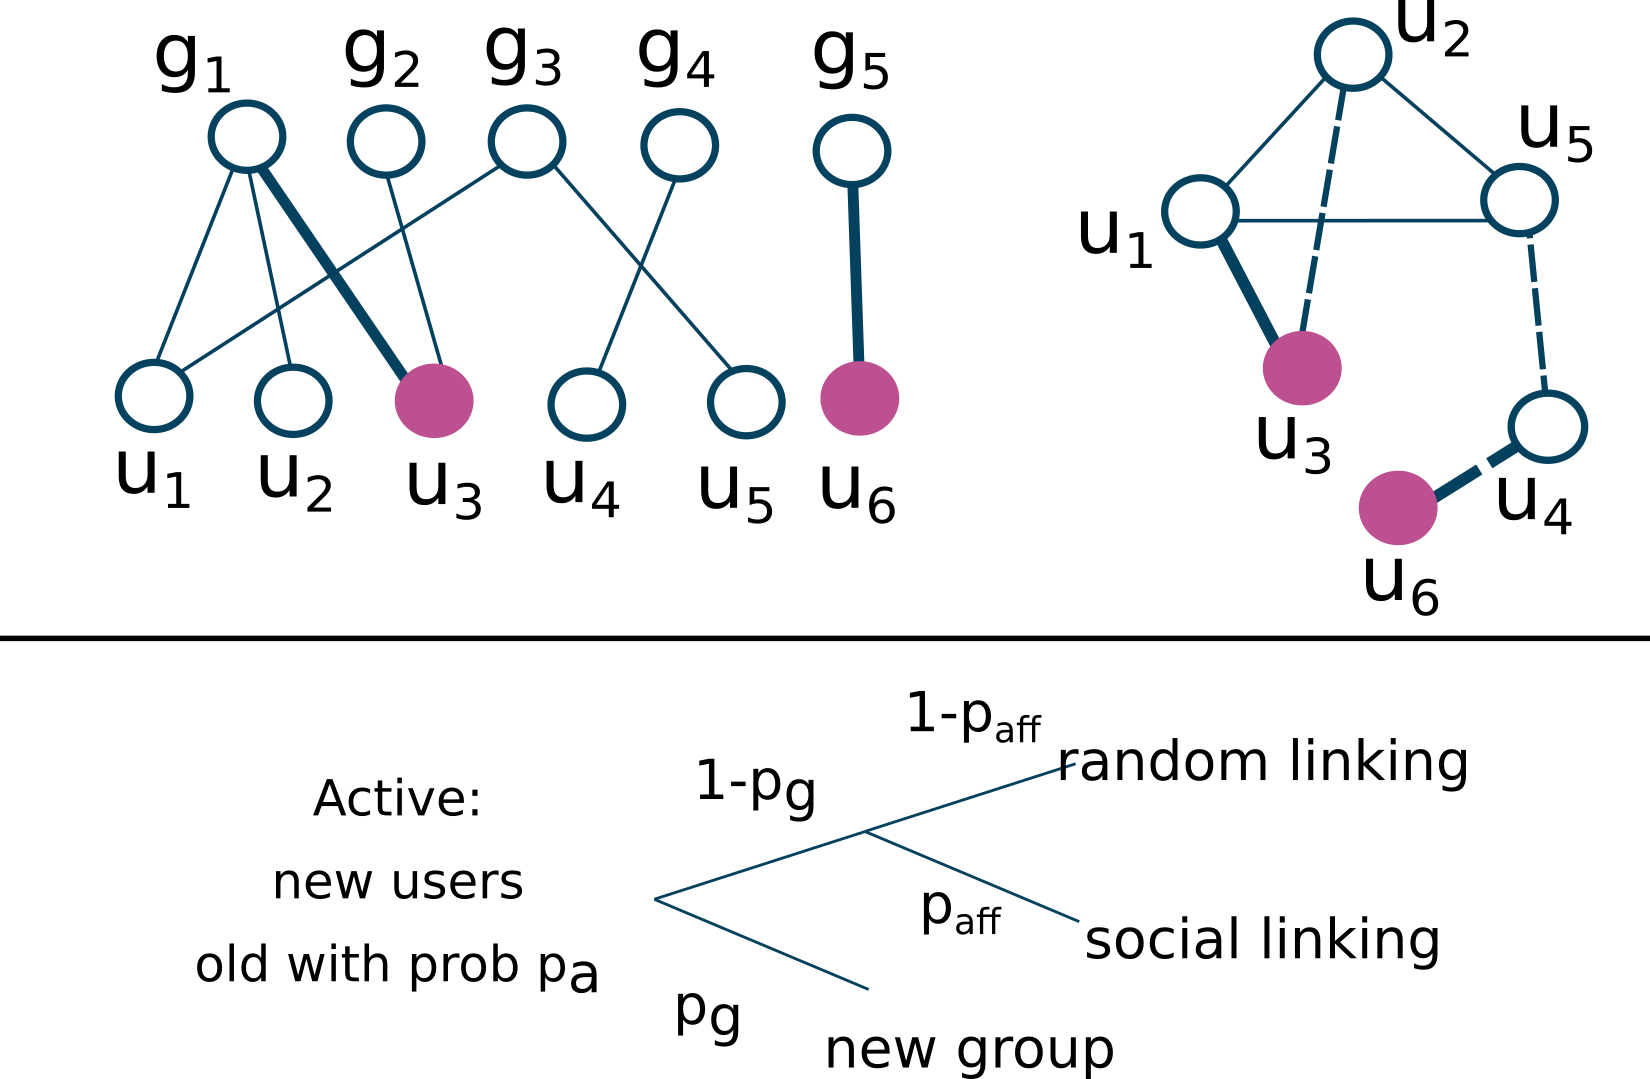
\includegraphics[scale=0.5]{Figures/test.png}
	\caption{The top panel shows bipartite (user-group) and social (user-user) network. Filled nodes are active users, while thick lines are new links in this time step. In the social network dashed lines show that users are friends but still do not share same groups. The lower panel shows model schema. \textbf{Example:} user $u_6$ is new user. First it will make random link  with node $u_4$, and then with probability $p_g$ makes new group $g_5$. With probability $p_a$ user $u_3$ is active, while others stay inactive for this time step. User $u_3$ will with probability $1-p_g$ choose to join one of old groups and with probability $p_{aff}$ linking is chosen to be social. As its friend $u_2$ is member of group $g_1$, user $u_3$ will also join group $g_1$. Joining group $g_1$, user $u_3$ will make more social connections, in this case it is user $u_1$.}
	\label{fig:my_label}
\end{figure}

This model can be easily adapted to follow the arbitrary number of new users at each time step. The parameters $p_a$ and $p_g$ determine the number of groups in the network, while with $p_{aff}$ the shape of group sizes distribution can be modified. If  $p_{aff}=0$ the linking mechanism is random and the distribution of groups sizes follow lognormal. With higher affiliation parameter distribution becomes broader, with larger variance. 


\section{Results \label{sec:results}}

For each group, we selected time point when user becomes the member. Looking into whole set of groups during selected time period, we can determine if user is active for the first time (new users) or it is already member of other groups (old user). Also, we can track the number of new groups. To simulate reddit and meetup network, we can approximate some parameters from real data. The time series of the new users can be directly incorporated in the model. Probabilities that old users are active $p_a$ and that new groups are created $p_g$ can be approximated from the data as $p_a = median [\frac{N_{old}(t)}{N(t)}]$, 
$p_g = median [\frac{Ng_{new}(t)}{N_{new}(t)+N_{old}(t)}]$, 
where $N$ is cumulative number of users in the network, $N_{old}$ is number of old active users while $N_{new}$ is number of new active users. The number of new groups is denoted as $Ng_{new}$.
We calculated the following parameters:
Meetup $p_a=0.05$, $p_g=0.003$, for Reddit $p_a=0.1$, $p_g=0.003$. 
We run the simulation with time series of new users, fixed parameters $p_a$ and $p_g$, while we vary affiliation parameter. We discovered that in meetup users are more likely to join groups randomly, the best model fit to data is found for small affiliation parameter 0.1. On the other hand, distribution of sizes for the Reddit network is better approximated with the higher affiliation parameter $p_{aff}=0.9$



\begin{figure}[h!]
	\centering
	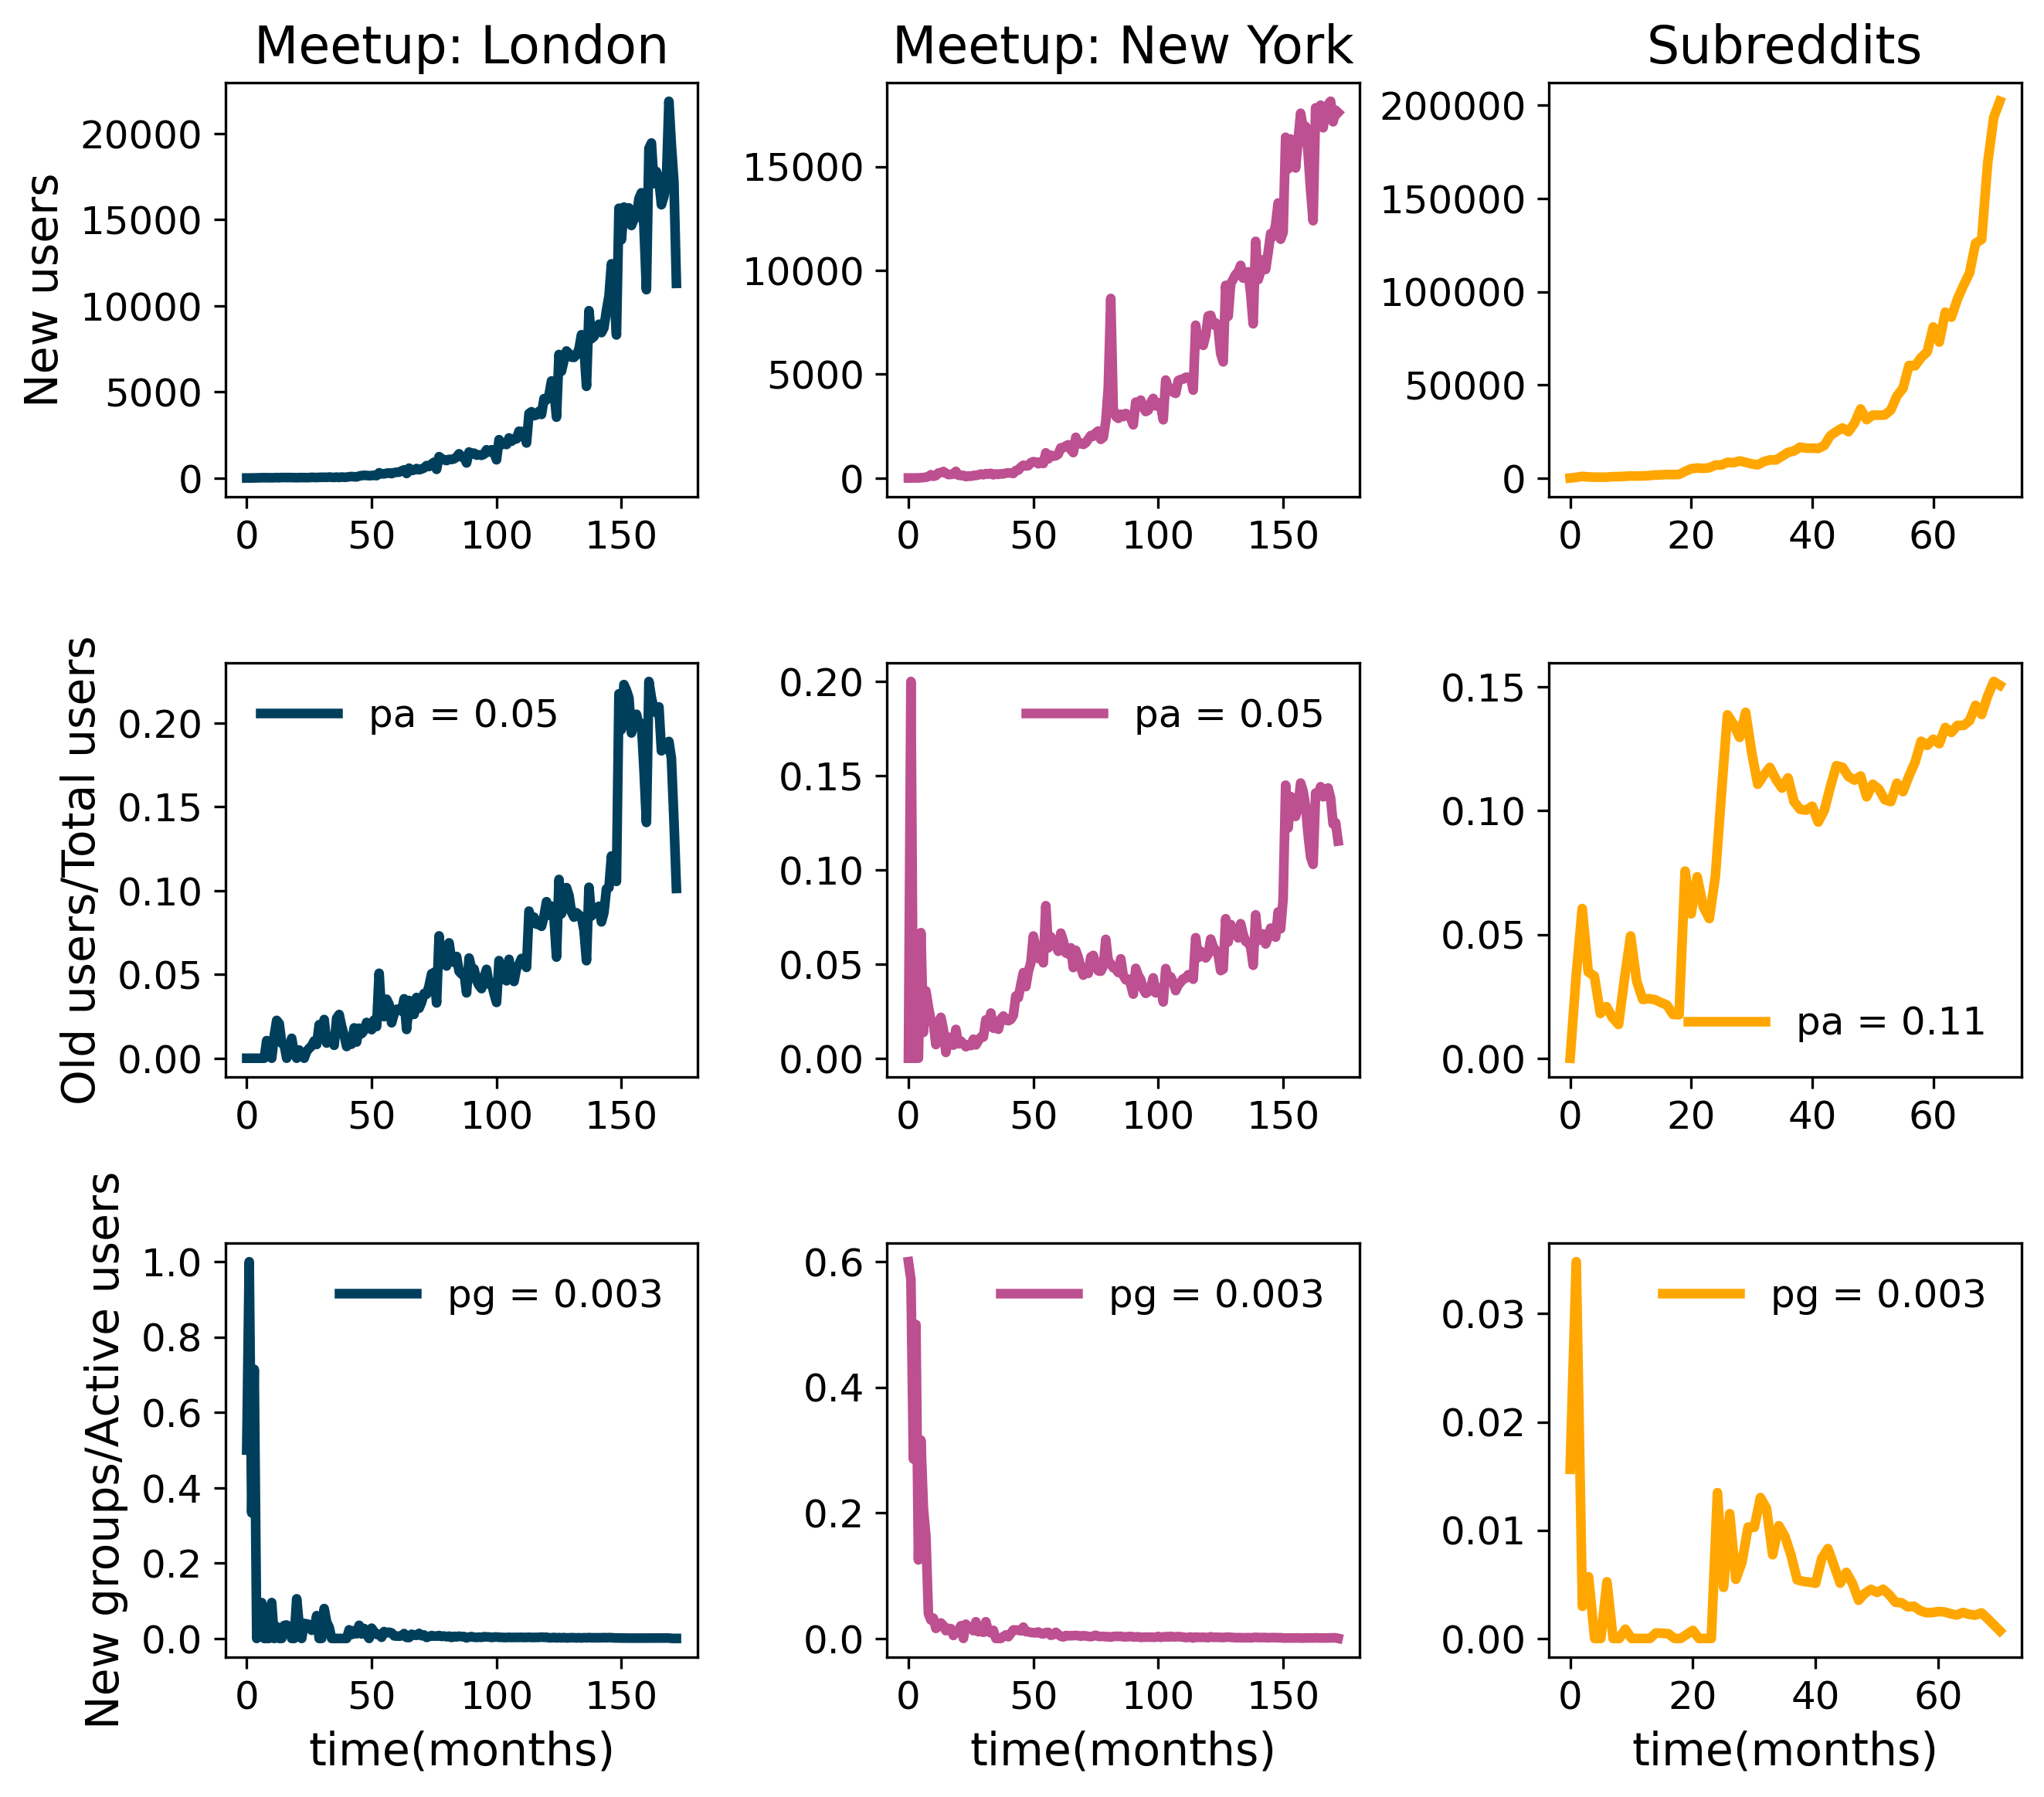
\includegraphics[width=0.6\linewidth]{Figures/Fig3.png}
	\caption{}
	\label{fig:fig3}
\end{figure}

\begin{figure}[h!]
	\centering
	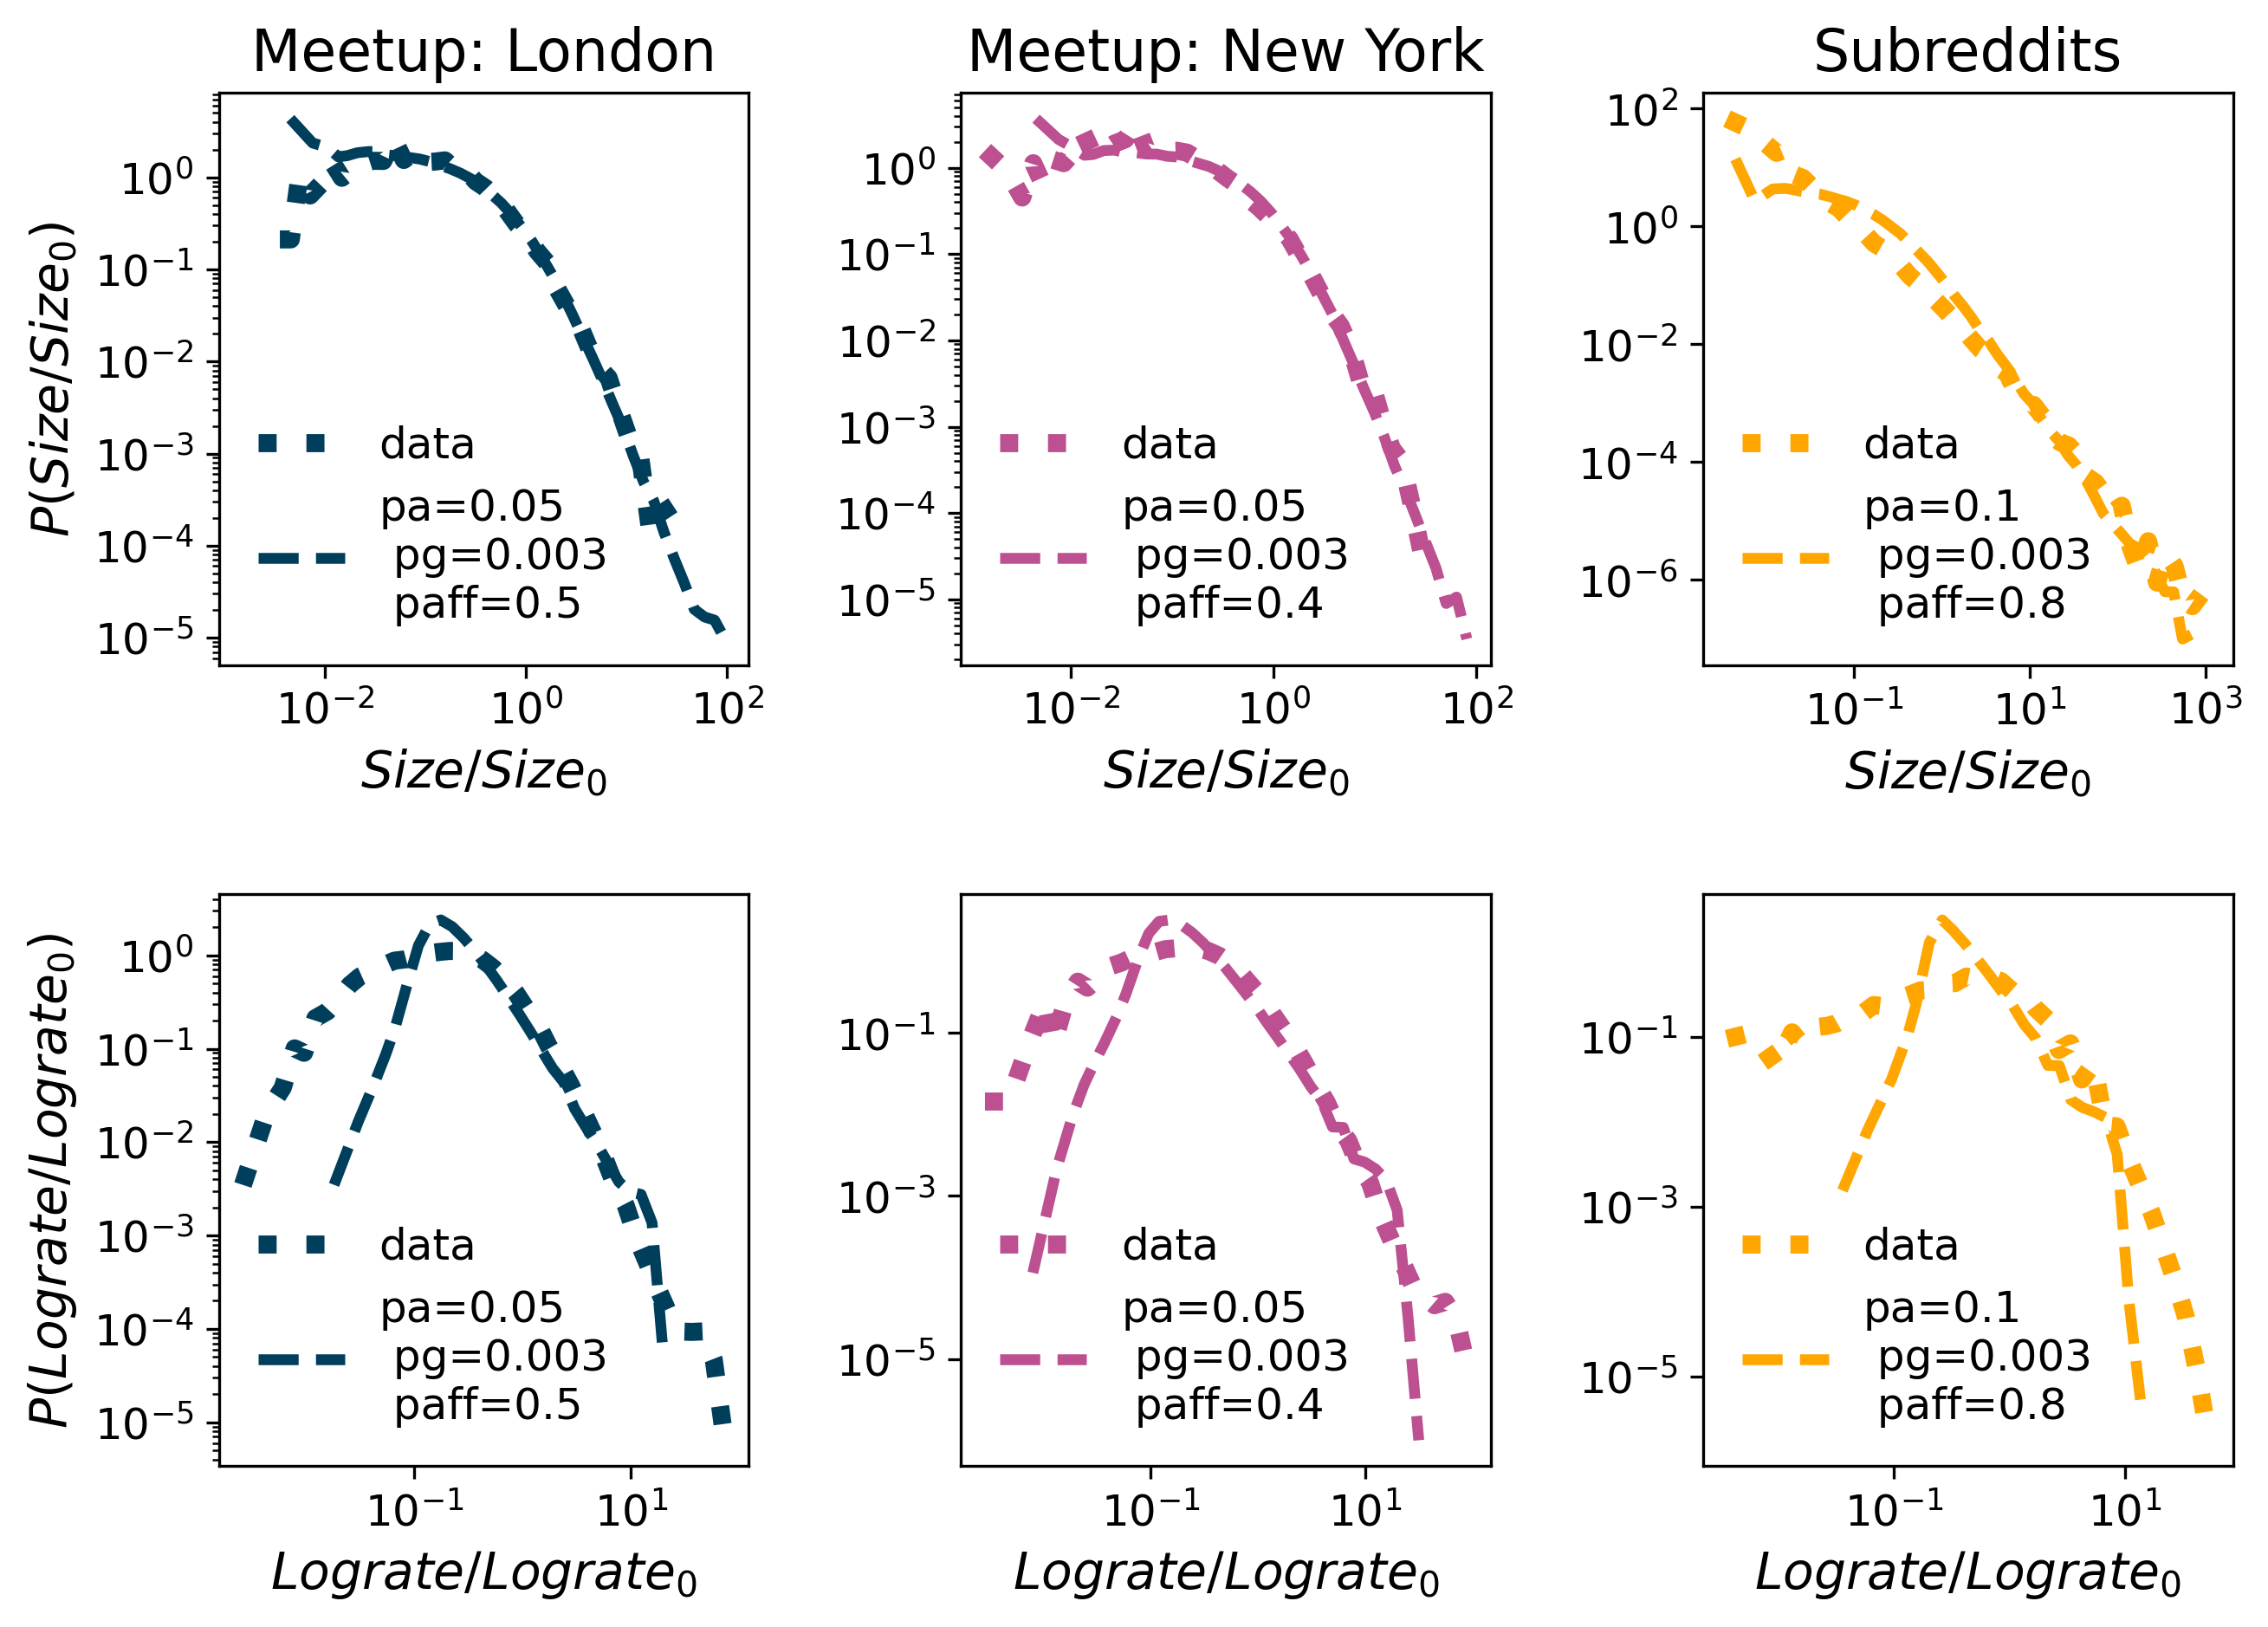
\includegraphics[width=0.6\linewidth]{Figures/Fig4.png}
	\caption{}
	\label{fig:fig4}
\end{figure}

\begin{table}[]
	\centering
	\begin{tabular}{c|c|c|c | c|c |c| c| c | c}
		
		paff & 0.1 & 0.2 & 0.3 & 0.4 & 0.5 & 0.6 & 0.7 & 0.8 & 0.9  \\
		\hline
		JS cityLondon & 0.0161 & 	0.0101  &	0.0055 &	0.0027  &	\textbf{0.0016} & 	0.0031 & 	0.0085  &	0.0214 & 	0.0499 \\
		JS cityNY & 0.0097 &	0.0053 & 	0.0026 &	\textbf{0.0013} & 	0.0015 & 	0.0035 & 	0.0081 & 	0.0167 &	0.0331 \\
		JS reddit2012 & - & - & - & - &  0.00074 & 0.00048 & 0.00039 & \textbf{0.00034} & 0.00047 \\
	\end{tabular}
	\caption{Jensen Shannon divergence between group sizes distributions from model (in model we vary affiliation parameter paff) and data. }
	\label{tab:my_label}
\end{table}

%----------------------------------------------------------------------------------------





\chapter{Stack Exchange} % Main chapter title

\label{Chapter3}

\section{Stack Exchange Data}

We focus the analysis on pairs of closed and active SE communities matched by topic. Astronomy, Literature, and Economics are currently active communities in the public beta phase. All three communities thrived the second time they were proposed. The first attempt to create communities on these topics was unsuccessful, and they were closed within a year. We add to the comparison the early days of Physics community and compare its evolution with the closed Theoretical Physics community. These communities do not have identical topic, but it is safe to assume that there is a high overlap of users' demographics and interests. For these reasons, we treat this pair in the same manner as others.\\ 
The Stack Exchange data are publicly available and released in a regular time intervals. We are primarily interested in activity and interaction data, which means we extract the following information for posts (questions and answers) and comments: 1) for all posts we extract unique ID; 2) for each post or comment we extract the time of its creation and unique ID its creator - user; 3) for every question we extract information about IDs of all answers to that question and ID accepted of accepted question; for each question or answer we collect information about IDs of comments related to that question or answer. The data contains information about the official StackExchange reputation of each user but only as a single value measuring the final reputation of the user on a day when data archive was released. Because of this significant shortcoming, we do not include this information in our analysis. In SE users can give positive or negative votes to questions and answers, and mark questions as favor, however the data is again provided as a final score recorded at the moment of the realise of the database. Since this does not allows us to analyse the evolution of scores, we omit this data from our analysis.\\



\begin{table}[h]
	%\footnotesize\sf\centering
	\caption{Community overview for first 180 days }
	\label{tab:site-info}
	\begin{tabular}{llccccc}
		\hline
		Site                 & Status                           & First Date                     & $n_u$                    & $n_q$                & $n_a$                  & $n_c$ \\ \hline
		\multirow{2}{*}{Astronomy}  & \multicolumn{1}{l|}{Closed}      & \multicolumn{1}{c|}{09/22/10} & \multicolumn{1}{c|}{336}  & \multicolumn{1}{c|}{474}  & \multicolumn{1}{c|}{953}  & 1444     \\
		& \multicolumn{1}{l|}{Beta} & \multicolumn{1}{c|}{09/24/13} & \multicolumn{1}{c|}{405}  & \multicolumn{1}{c|}{644}  & \multicolumn{1}{c|}{959}  & 2170     \\ \hline
		\multirow{2}{*}{Economics}  & \multicolumn{1}{l|}{Closed}      & \multicolumn{1}{c|}{10/11/10} & \multicolumn{1}{c|}{275}  & \multicolumn{1}{c|}{368}  & \multicolumn{1}{c|}{458}  & 1253     \\
		& \multicolumn{1}{l|}{Beta} & \multicolumn{1}{c|}{11/18/14} & \multicolumn{1}{c|}{648}  & \multicolumn{1}{c|}{1024} & \multicolumn{1}{c|}{1410} & 3553     \\ \hline
		\multirow{2}{*}{Literature} & \multicolumn{1}{l|}{Closed}      & \multicolumn{1}{c|}{02/10/10} & \multicolumn{1}{c|}{284}  & \multicolumn{1}{c|}{318}  & \multicolumn{1}{c|}{523}  & 1097     \\
		& \multicolumn{1}{l|}{Beta} & \multicolumn{1}{c|}{01/18/17} & \multicolumn{1}{c|}{478}  & \multicolumn{1}{c|}{910}  & \multicolumn{1}{c|}{907}  & 3301     \\ \hline
		\multirow{2}{*}{Physics}    & \multicolumn{1}{l|}{Closed}      & \multicolumn{1}{c|}{09/14/11} & \multicolumn{1}{c|}{281}  & \multicolumn{1}{c|}{349}  & \multicolumn{1}{c|}{564}  & 2213     \\
		& \multicolumn{1}{l|}{Launched}    & \multicolumn{1}{c|}{08/24/10} & \multicolumn{1}{c|}{1176} & \multicolumn{1}{c|}{2124} & \multicolumn{1}{c|}{4802} & 15403    \\
		\bottomrule
	\end{tabular}
	{\raggedright \textit{Note:} Number of users $n_u$, number of questions $n_q$, number of answers $n_a$, number of comments $n_c$ \par}
	
\end{table}
The beginning of each SE community is the same. In a \textit{Definition} phase a small number of SE users starts with designing communities by proposing hypothetical questions about a certain topic. A successful \textit{Definition} phase is followed by a \textit{Commitment} phase. In this phase interested users commit to the community to make it more active. The \textit{Beta} phase, that follows after the \textit{Commitment} phase, is the most important. It consists of two steps: a three week private beta phase, where only committed users may ask/answer/comment questions; and public beta phase when other members are allowed to join the community. The duration of public beta phase is not limited. However, every 90 days the community is evaluated. Depending on this analysis there are three possible outcomes: 1) the community is considered successful and it graduates; 2) community is alive but needs more work to graduate, which means that public beta phase continues; 3) the community died and the site is closed. Community evaluation/review process is guided by simple metrics: average number of questions per day, average number of answers per question, percentage of answered questions, total number of users and number of avid users, and average number of visits per day.\\

We study how social network-related properties of these social communities and the social trust created among their members evolve during the first six months. First 90 days are recognised as minimal amount of time that a newly established community should spend in the beta phase. We investigate twice as long period, since closed communities were active between 180 and 210 days. Given that differences in first few months of online community lifetime can be predictive of community survival and evolution \cite{dover2020sustainable}, we are interested in early evolution of Stack Exchange sites. 

Basic information about gathered activities in first 180 days of community lifetime is shown in table \ref{tab:site-info}. Closed communities had fewer users, questions and comments in total during this period. Although the official review of Stack Exchange communities in beta phase is based on simple activity indicators such as number of questions or ratio of answers to questions\footnote{\href{https://stackoverflow.blog/2011/07/27/does-this-site-have-a-chance-of-succeeding/}{https://stackoverflow.blog/2011/07/27/does-this-site-have-a-chance-of-succeeding/}}, these simple metrics cannot provide insight about factors which influence the success of any given community. The Table S2 in SI, shows the values of some of these measures at 180 days point for considered communities. While Physics community was clearly more successful than Theoretical Physics and other considered communities, we see that these differences are not as clear if we compare three other pairs of communities. For instance, some of the parameters for closed Astronomy community were better than for the community that is still alive. Similar results were found for Economics and Literature. Another simple indicator can be the time series of active questions for the period of 7 days shown in Fig \ref{fig:active_questions}. The question is considered to be active if it had at least one an activity, posted answer or comment, during the previous 7 days. All four pair of compared communities show that live communities have larger number of active questions after the first three months of community existence. While this difference is striking for Physics and Economics community, Fig. \ref{fig:active_questions} shows that this difference is smaller for Astronomy and Literature community. Furthermore, we observe that in the case of Astronomy, closed community had higher number of active questions in the first 75 days. \\
The values of measures shown in Table \ref{tab:site-info} and S2, and Fig. \ref{fig:active_questions} suggest that these simple measures are not sufficient indicators about the community long-term sustainability, and that we need deeper insights into community structure and dynamics to understand the factors behind the sustainability of these communities. The structure of social interactions within communities and dynamics of collective trust may provide better explanation of why certain communities thrive and others die.  

%Ovde nemamo ni jedan dodatak u SI. Razmišljam da ove indikatore stavimo u SI?

% da li da preciziramo sta je active question ili je jasno?

\begin{figure*}
	\centering
	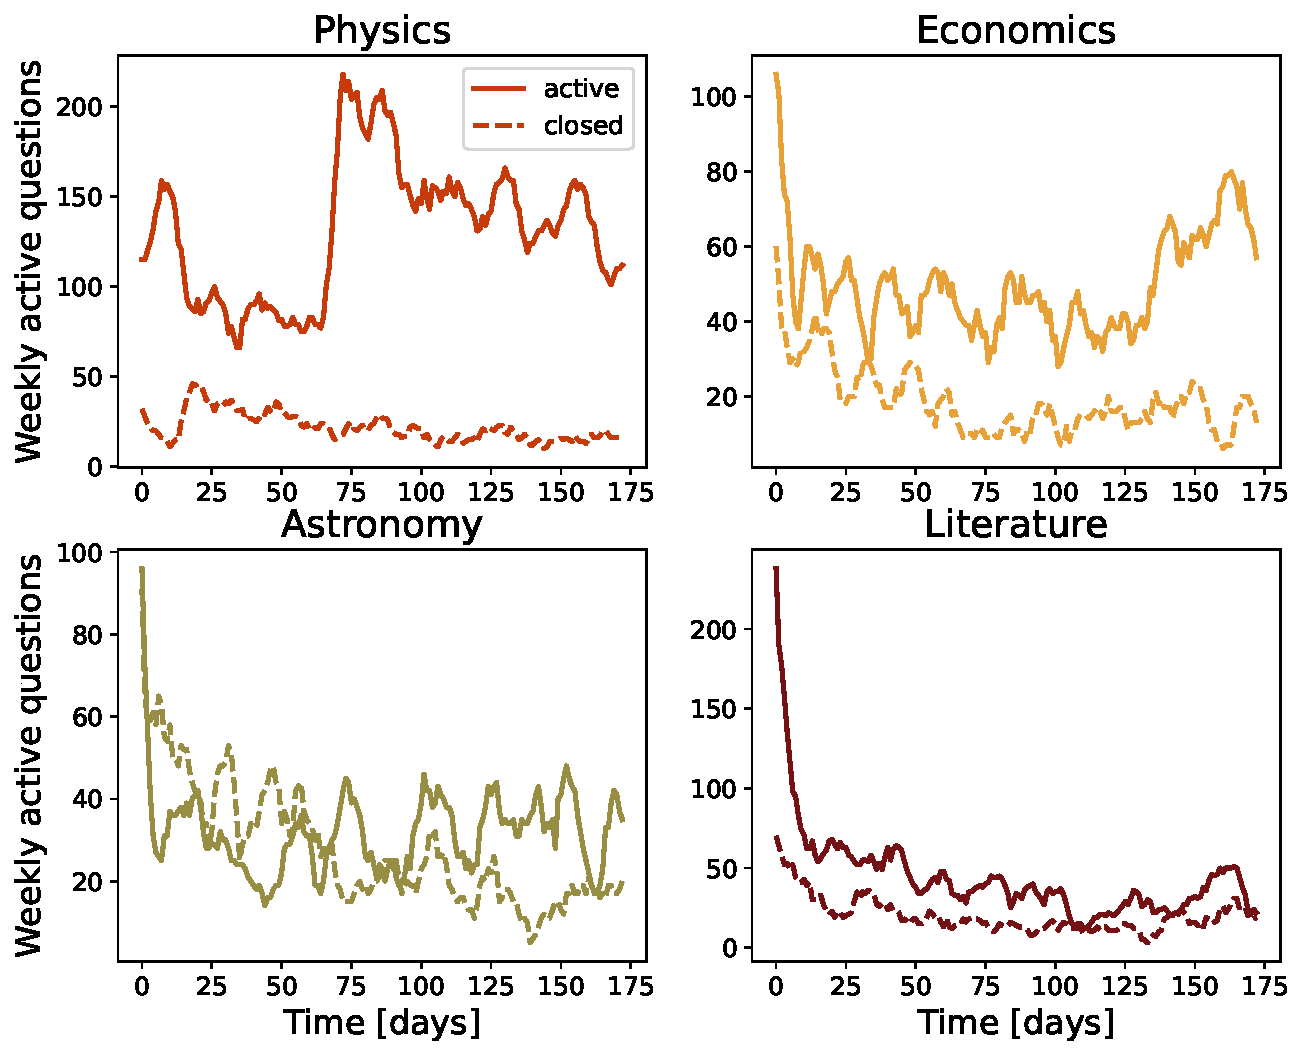
\includegraphics[width=0.5\linewidth]{Figures/figures_SE/Fig2.pdf}
	\caption{Number of active questions within 7 days sliding windows. Solid line - active sites; dashed lines - closed sites.}
	\label{fig:active_questions}
\end{figure*}



\subsection{Negative interactions}

The average percentage of negatively voted interactions is 3.2\% for questions and 3\% for answers. Percentages for questions and answers from each community are shown in table \ref{tab:negint}.  Comments cannot have negative vote sum as they can only be upvoted.

\begin{table}[hbt!]
	\centering
	\caption{Percentage of negatively voted interactions}
	\label{tab:negint}
	\begin{tabular}{@{}ccc@{}}
		\toprule
		Community           & Questions & Answers \\ \midrule
		Physics Launched    & 5\%       & 4\%     \\
		Physics A51         & 1\%       & 2\%     \\
		Astronomy Launched  & 3\%       & 3\%     \\
		Astronomy A51       & 2\%       & 1\%     \\
		Economics Launched  & 4\%       & 4\%     \\
		Economics A51       & 7\%       & 4\%     \\
		Literature Launched & 2\%       & 5\%     \\
		Literature A51      & 2\%       & 1\%     \\ \midrule
		\textbf{Average}    & 3.2\%     & 3\%     \\ \bottomrule
	\end{tabular}
\end{table}


\subsection{Area51 criteria}

The Stack Exchange has its own criteria for the success of sites. They measure how many questions are answered, how many questions are posted per day, and how many answers are posted per question.  There are two measures: the number of avid users and the number of visits that are not easily interpreted from the data. The site is \textit{healthy} if it has 10 questions per day, 2.5 answers per question and more than $90\%$ of answered questions. For less than $80\%$ of answered questions, 5 questions per day and 1 question per answer site \textit{needs some work}. We calculated Stack Exchange statistics for astronomy, economics, literature and physics and results are presented in the table 1. After 180 days only beta physics is healthy site while other betas are at least in two criteria labeled as \textit{okay}. Closed sites mostly \textit{need some work}, the exception is closed astronomy with \textit{excellent} percent of answered questions and \textit{okay} answer ratio. 

\begin{table}[h!]
	%\footnotesize\sf\centering
	\caption{Community overview for first 180 days according to SE criteria  }
	
	\label{tab:se_c}
	\begin{tabular}{ccccc}
		\hline
		
		Site & Status &  Answered & Questions per day & Answer ratio \\ \hline
		\multirow{2}{*}{Astronomy} & \multicolumn{1}{c|}{Closed} & \multicolumn{1}{c|}{\textbf{95} \%}  & \multicolumn{1}{c|}{2.62} & \multicolumn{1}{c}{\underline{2.02}} \\
		& \multicolumn{1}{c|}{Beta} & \multicolumn{1}{c|}{\textbf{96} \%}  & \multicolumn{1}{c|}{3.57} & \multicolumn{1}{c}{\underline{1.49}} \\ \hline
		\multirow{2}{*}{Economics} & \multicolumn{1}{c|}{Closed} & \multicolumn{1}{c|}{68 \%}  & \multicolumn{1}{c|}{2.04} & \multicolumn{1}{c}{\underline{1.25}} \\
		& \multicolumn{1}{c|}{Beta} & \multicolumn{1}{c|}{\underline{84} \%}  & \multicolumn{1}{c|}{\underline{5.66}} & \multicolumn{1}{c}{\underline{1.37}} \\ \hline
		\multirow{2}{*}{Literature} & \multicolumn{1}{c|}{Closed} & \multicolumn{1}{c|}{79 \%}  & \multicolumn{1}{c|}{1.77} & \multicolumn{1}{c}{\underline{1.65}} \\
		& \multicolumn{1}{c|}{Beta} & \multicolumn{1}{c|}{74 \%}  & \multicolumn{1}{c|}{\underline{5.04}} & \multicolumn{1}{c}{\underline{1.10}} \\ \hline
		\multirow{2}{*}{Physics} & \multicolumn{1}{c|}{Closed} & \multicolumn{1}{c|}{83 \%}  & \multicolumn{1}{c|}{1.93} & \multicolumn{1}{c}{\underline{1.64}} \\
		& \multicolumn{1}{c|}{Beta} & \multicolumn{1}{c|}{\textbf{93} \%}  & \multicolumn{1}{c|}{\textbf{11.76}} & \multicolumn{1}{c}{ \textbf{2.74}} \\ \hline \hline
		{Stack Exchange criteria} & excellent & $>$ 90 \% & $>$10 & $>$ 2.5   \\
		& needs some work & $<$ 80 \% & $<5$ & $<$ 1   \\ \hline
		
		
	\end{tabular}
	
\end{table}

\clearpage

\section{Properties of Stack Exchange data}

We examine the differences between live and closed communities by analysing network properties and dynamic of collective trust. We are particularly interested in the position of trustworthy members in these communities and whether there are differences between live and close communities. For these reasons, we map the interaction data onto networks and analyse their network properties. We use dynamical reputation model to estimate the trustworthiness of each member of community.     

\subsection{Network mapping}
%{\color{blue} Here we need a description how we map the data onto networks, why sliding windows $30$days, sliding windows, etc....}

%From Stack Exchange data, we selected questions, answers and comments. Each post is associated with the user-id and timestamp. 
%ovo gore sam iskomentarisala zato sto postoji u data sekciji
We treat all user interactions (answering questions, posting questions or comments, accepting answers) as equal. We construct a network of users where the link between two nodes (users) $i$ and $j$ exists if: $i$ answers or comments question posted by $j$ and vice verse, or $i$ comments answer posted by $j$ and vice verse. We do not consider the direction or the frequency of the interaction between users $i$ and $j$, and thus, we create unweighted and uncorrelated network. 
%This is probably not good enough argument…
We study how properties of networks evolve in the first 180 days of the community life. We create a network snapshot $G(t, t+\tau$) at the time $t$ for the time window length $\tau$. Two users $(i, j)$ are connected in a network snapshot $G(t, t+\tau$) if they had at least one interaction during the time $[t,t+\tau]$. We create 150 interaction networks, our first network accounts for interaction within the first 30 days $G[0,30)$ and we slide the window of interaction by one day and finish with $G[149,179)$ network. By sliding the time window by one day we create two consecutive networks that overlap significantly. This way we are able to to capture fine structural changes that are consequences of daily added/removed interactions. We calculate different structural properties of these networks and analyse how they change over the period of 180 days.  


There is no well-specified procedure for the choice of sliding window $\tau$. Previous studies showed that if $\tau$ is small sub networks become sparse, while for too large sliding windows some important structural changes can not be observed \cite{krings2012effects, arnold2021moving}. We analyse how networks properties and properties of dynamical reputation change with the window size, see SI for more details. Figure A13 in SI shows how considered network properties and dynamical reputation depend on the time window size for active and closed communities on the astronomy. We observe that fluctuations of all measures are more pronounced for time window of 10 days than for 30 and 60 days. However, we find that while the structural properties of networks evolve at different paces over varied time windows the trends remain very similar. The observed qualitative difference between closed and live communities is independent of $\tau$, especially if we compare time window size of 30 and 60 days. The time window size of 30 days ensures enough amount of interaction, even for closed communities, while the number of observation points remains relatively high. For these reasons, we choose a sliding window of 30 days. 

\subsection{Clustering}
There are many local and global measures of network properties \cite{boccaletti2006complex}. These measures are not independent. However, it was shown that degree distribution, degree-degree correlations and clustering coefficient are sufficient to fully describe most of the complex networks including social networks \cite{orsini2015quantifying}. The clustering coefficient of a node quantifies the average connectivity of between its neighbours and cohesion of its neighbourhood \cite{boccaletti2006complex}. It is a probability that two neighbours of a node are also neighbours, and is calculated using the following formula:
\begin{equation}
c_{i}=\frac{e_{i}}{\frac{1}{2}k_{i}(k_{1}-1)} \ .
\label{eq:clust}
\end{equation}
Here $e_{i}$ is the number of links between neighbours of the node $i$ in a network, while $\frac{1}{2}k_{i}(k_{i}-1)$ is the maximal possible number of links determined by the node degree $k_{i}$. The clustering coefficient of network $C$ is the value of clustering averaged over all nodes. Here we investigate how clustering coefficient in a SE community is changing with time by calculating its value for all network snapshots. We compare the behavior of clustering for active and closed communities on the same topic in order to better understand how cohesion of these communities is changing over time. 
Members' clustering coefficient measures the probability that other members connected to them are also connected. Study on dynamics of social group growth shows that that links between one's friends that are members of a social group increase the probability that that individual will join the social group \cite{backstrom2006group}. Furthermore, successful social diffusion  typically occur in networks with high value of clustering coefficient \cite{centola2007cascade}. These results suggest that high local cohesion should be a characteristic of sustainable communities.

\subsection{Core-periphery structure}

Real networks, including social networks, have a distinct mesocopic structure \cite{fortunato2010community, gallagher2020clarified}. Mescoscopic structure is manifested either through community structure or core-periphery structure. Networks that have community structure consist of a certain number of group of nodes that are densely connected with each other, with sparse connections between groups. Networks with core-periphery structure consist of two groups of nodes, with higher edge density within one group and between groups but low edge density in the second group \cite{gallagher2020clarified}. Research on dynamics of user interaction in SE communities shows that there is a small group of highly active members, similar to core,  that have frequent interactions with casual or low active members of community \cite{santos2019activity, santos2019self}. These results indicate that we should expect a core-periphery structure in SE communities. 

Core-periphery pattern means that network consists of two components: a core, densely connected group of nodes, and periphery, a second group of nodes that are loosely connected with the core and with each other. Classification of nodes into one of these two groups provide us with information about their functional and dynamical roles in the network. Active users typically belong to core, while periphery consists of less active users.

To investigate core-periphery structure of SE communities and how it evolves trough time, we analyse the core-periphery structure of every 30 days network snapshot. We use Stochastic Block Model (SBM) adapted for core-periphery inference of network structure \cite{gallagher2020clarified} to determine the core-periphery structure.  

\textbf{SBM} is model where each node, in given network G,  belongs to one of $B$ blocks. Vector $\theta_i = r$ indicates that node $i$ is in block $r$, while SBM matrix $\{p\}_{BxB}$, specify the probability $p_{rs}$ that nodes from group $r$ are connected to nodes in group $s$. The SBM model is looking for the most probable model that can reproduce a given network G. Probability of having model parameters $\theta, p$ given network $G$ is proportional to likelihood of generating network $G$, prior of SBM matrix and prior on block assignments:

\begin{equation}
P(\theta, p| G) = P(G | \theta , p) P(p) P(\theta) 
\end{equation}

\begin{equation}
P(G | \theta , p) = \prod_{i<j} p_{r_is_j}^{A_{ij}}(1-p_{r_is_j})^{1-A_{ij}}  
\end{equation}

where $A_{ij}$ is number of edges between nodes $i$ and $j$. 

Prior on p is modified for core-periphery model such that $P(p) = 3!I_{0<p_{22}<p_{12}<p_{11}<1}$, while prior on $\theta $ consists of three parts: probability of having $l$ blocks; given the number of layers probability $P(n|l)$ of having groups of sizes ${n_1..n_l}$ and the probability $P(\theta|n)$ of having particular assignments of nodes to blocks. 

For fitting model in the work \cite{gallagher2020clarified} authors use Metropolis-within-Gibbs algorithm.
The likelihood of SBM model increase with number of blocks and model itself does not define optimal number of communities. Inferring minimum description length
of the model is one approach to decide which model is more likely.  

%\subsection{Core-periphery sample}
For each 30 days snapshot network we run 50 iterations and choose the model parameters $\theta$ and $p$ according to minimum description length. MDL does not change much among inferred core-periphery structure, see Fig. A8, while looking into adjusted rand index we can notice that difference exists. Still, ARI between pair-wised compared partitions is large ($ari >0.9$) indicating stability of inferred structures.

\subsection{Clustering and core-periphery structure of knowledge-sharing networks}

We first analyse structural properties of Stack Exchange communities and examine the difference between successful and unsuccessful ones. We calculate the mean clustering coefficient for 30-days window networks and examine how it changes with time. Figure \ref{fig:clustering} shows the evolution of mean clustering coefficient for all eight communities. All communities that are still alive are clustered, with the value of mean clustering coefficient higher than 0.1. Physics, the only launched community, has the value of clustering coefficient above 0.2 for the first 180 days.
During larger part of the observed period, the clustering coefficient of an active community is higher compared to the clustering coefficient of its closed pair. If we compare active communities with their closed counterpart, the closed communities have higher value of the mean clustering coefficient in the early phase while later communities that are still active have higher values of clustering coefficient. These results suggest that all communities have relatively high local cohesiveness, and that lower values of clustering coefficient in the later phase of community life may be an indicator of its decline. 

\begin{figure}
	\centering
	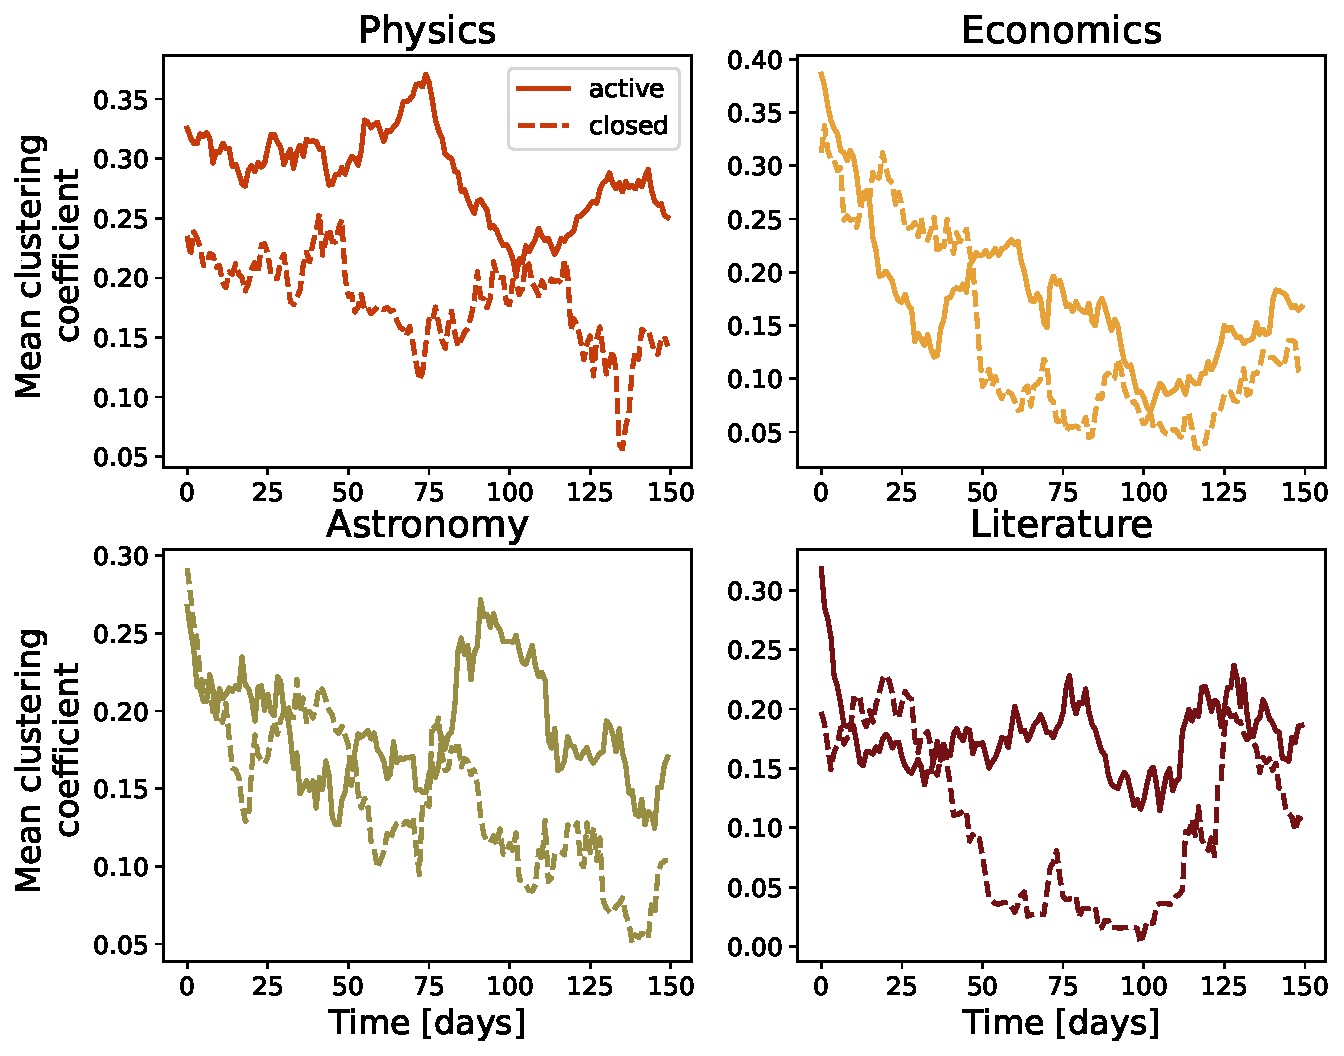
\includegraphics[width=\linewidth]{Figures/figures_SE/Fig3.pdf}
	\caption{Mean clustering coefficient.}
	\label{fig:clustering}
\end{figure}
Furthermore, we examine core-periphery structure of these communities and its evolution. Specifically, we are interested in the evolution of connectivity in the core. Figure \ref{fig:links_per_node} shows the number of links between nodes in the core per node $\frac{L}{N}(t)$. $\frac{2L}{N}$ is the average degree of the node in the core, and thus, $\frac{L}{N}$ is the half of the average degree. Again, Physics community has the much higher value of this quantity than Theoretical physics during the whole observed period, indicating higher connectivity between core members. Higher connectivity between core members in the active community is also characteristic for Literature, although this quantity has the same value for active and closed communities at the end of the observation period. The differences between active and closed communities are not that evident for Economics and Astronomy, see Fig. \ref{fig:links_per_node}. Active and closed Economics communities have similar connectivity in the core during the first 50 days. After this period, the connectivity in the core of the active community the twice as large as in the closed community and the difference grows at the end of observation period. The connectivity in the core of closed Astronomy community is higher that the connectivity in the core of the active community during the first 50 days. But as the time progresses, this difference changes in the favor of live community, while at the end of the observation period the difference disappears.

The difference between active and closed communities is more prominent if we consider average number of core-periphery edges per core node. The connectivity between core and periphery is higher for the still active communities than for the closed ones, see Fig. \ref{fig:links_per_node}. This is very obvious if we compare Physics and Theoretical physics community. Moreover, Physics community has the highest connectivity compared to all other communities. When it comes to active communities that are still in the beta phase, they either have the same core-periphery connectivity as their closed counter part, or as in the case of Astronomy, their periphery is weaker connected to the core during the first 50 days of their life, see Fig. \ref{fig:links_per_node}. 

On average, the cores of the active communities have higher number of nodes in the core than the closed communities, Fig. A11. However, the relative size of the core compared to the size of the whole network is similar when we compare closed and active communities on the same topic. This is even true for communities on physics topic. The size of the core fluctuates with time for active and closed communities. The core membership also changes with time. This core membership is changing more for the closed communities. We quantify this by calculating the Jaccard index between the cores of the subnetworks in the moment $t_{i}$ and $t_{j}$. Figure A9 in Supplementary Information shows the value of Jaccard index between any two of the 150 subnetworks. The highest value of the Jaccard index is around the diagonal and has value close to 1. This is expected, since these subnetworks are for consecutive days and the difference between them is smaller. The value of Jaccard index decreases with number of days between two subnetworks $|t_{i}-t_{j}|$ faster in closed communities Fig. A10. This difference is the most prominent for the literature communities, while this difference is practically non-existent for Astronomy. The relatively high overlap between cores of even more distant subnetworks for active communities, further confirms that the core is more stable in these communities that in their closed counterparts. 


\begin{figure}
	\centering
	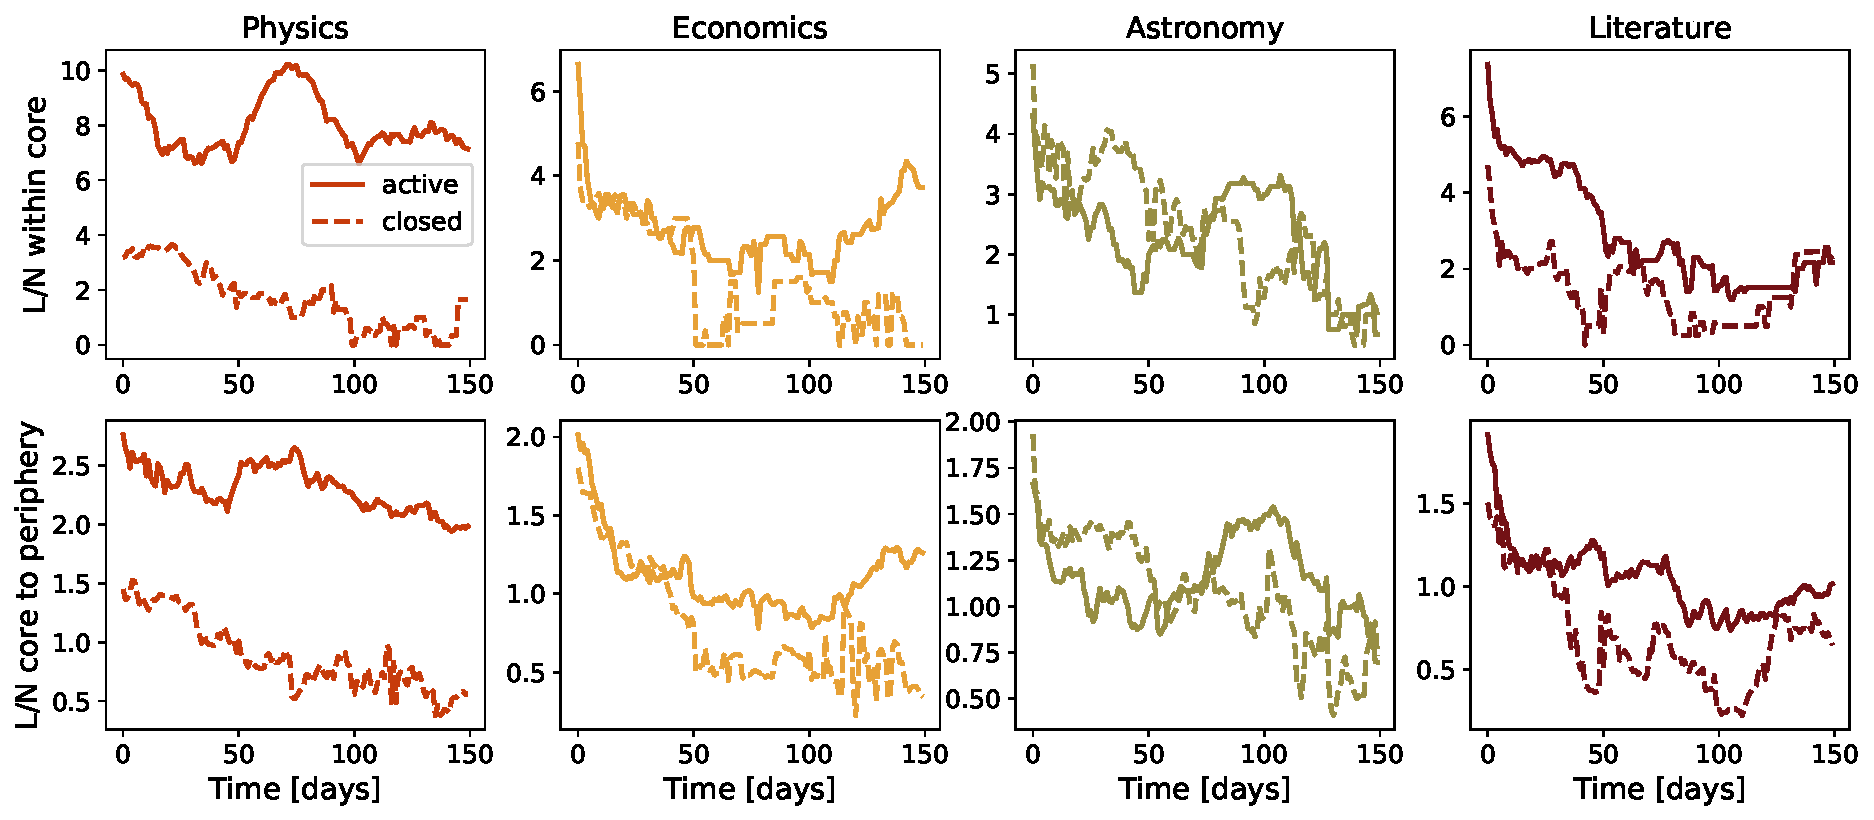
\includegraphics[width=\linewidth]{Figures/figures_SE/Fig5.pdf}
	\caption{Links per node in core and links per node between core and periphery.}
	\label{fig:links_per_node}
\end{figure}

\subsection{Clustering and core-periphery structure of knowledge-sharing networks}

We first analyse structural properties of Stack Exchange communities and examine the difference between successful and unsuccessful ones. We calculate the mean clustering coefficient for 30-days window networks and examine how it changes with time. Figure \ref{fig:clustering} shows the evolution of mean clustering coefficient for all eight communities. All communities that are still alive are clustered, with the value of mean clustering coefficient higher than 0.1. Physics, the only launched community, has the value of clustering coefficient above 0.2 for the first 180 days.
During larger part of the observed period, the clustering coefficient of an active community is higher compared to the clustering coefficient of its closed pair. If we compare active communities with their closed counterpart, the closed communities have higher value of the mean clustering coefficient in the early phase while later communities that are still active have higher values of clustering coefficient. These results suggest that all communities have relatively high local cohesiveness, and that lower values of clustering coefficient in the later phase of community life may be an indicator of its decline. 

\begin{figure}
	\centering
	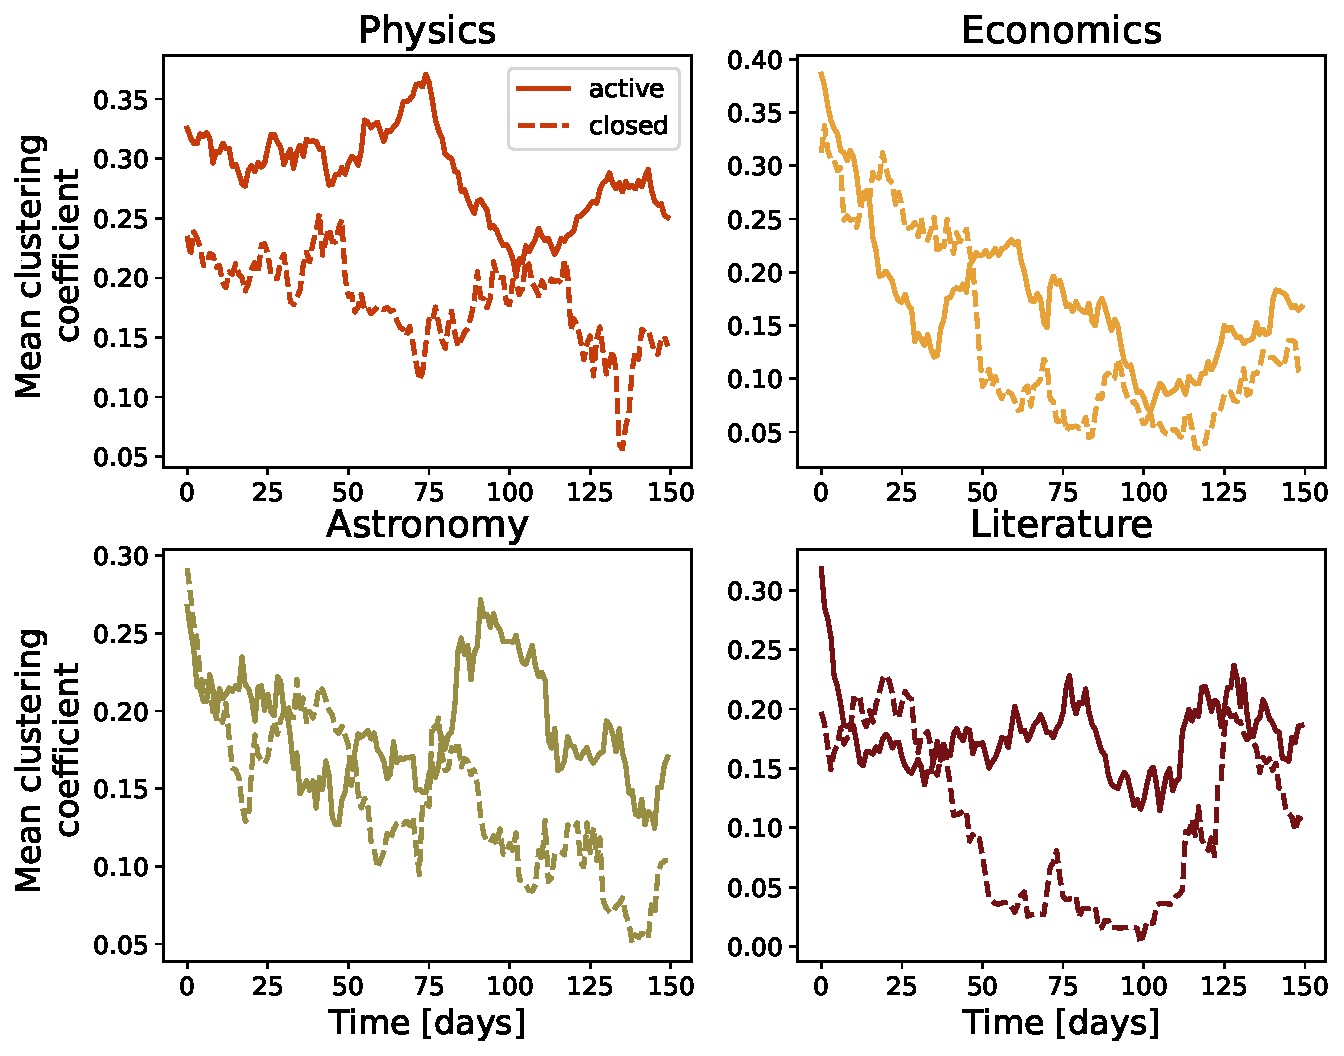
\includegraphics[width=\linewidth]{Figures/figures_SE/Fig3.pdf}
	\caption{Mean clustering coefficient.}
	\label{fig:clustering}
\end{figure}
Furthermore, we examine core-periphery structure of these communities and its evolution. Specifically, we are interested in the evolution of connectivity in the core. Figure \ref{fig:links_per_node} shows the number of links between nodes in the core per node $\frac{L}{N}(t)$. $\frac{2L}{N}$ is the average degree of the node in the core, and thus, $\frac{L}{N}$ is the half of the average degree. Again, Physics community has the much higher value of this quantity than Theoretical physics during the whole observed period, indicating higher connectivity between core members. Higher connectivity between core members in the active community is also characteristic for Literature, although this quantity has the same value for active and closed communities at the end of the observation period. The differences between active and closed communities are not that evident for Economics and Astronomy, see Fig. \ref{fig:links_per_node}. Active and closed Economics communities have similar connectivity in the core during the first 50 days. After this period, the connectivity in the core of the active community the twice as large as in the closed community and the difference grows at the end of observation period. The connectivity in the core of closed Astronomy community is higher that the connectivity in the core of the active community during the first 50 days. But as the time progresses, this difference changes in the favor of live community, while at the end of the observation period the difference disappears.

The difference between active and closed communities is more prominent if we consider average number of core-periphery edges per core node. The connectivity between core and periphery is higher for the still active communities than for the closed ones, see Fig. \ref{fig:links_per_node}. This is very obvious if we compare Physics and Theoretical physics community. Moreover, Physics community has the highest connectivity compared to all other communities. When it comes to active communities that are still in the beta phase, they either have the same core-periphery connectivity as their closed counter part, or as in the case of Astronomy, their periphery is weaker connected to the core during the first 50 days of their life, see Fig. \ref{fig:links_per_node}. 

On average, the cores of the active communities have higher number of nodes in the core than the closed communities, Fig. A11. However, the relative size of the core compared to the size of the whole network is similar when we compare closed and active communities on the same topic. This is even true for communities on physics topic. The size of the core fluctuates with time for active and closed communities. The core membership also changes with time. This core membership is changing more for the closed communities. We quantify this by calculating the Jaccard index between the cores of the subnetworks in the moment $t_{i}$ and $t_{j}$. Figure A9 in Supplementary Information shows the value of Jaccard index between any two of the 150 subnetworks. The highest value of the Jaccard index is around the diagonal and has value close to 1. This is expected, since these subnetworks are for consecutive days and the difference between them is smaller. The value of Jaccard index decreases with number of days between two subnetworks $|t_{i}-t_{j}|$ faster in closed communities Fig. A10. This difference is the most prominent for the literature communities, while this difference is practically non-existent for Astronomy. The relatively high overlap between cores of even more distant subnetworks for active communities, further confirms that the core is more stable in these communities that in their closed counterparts. 


\begin{figure}
	\centering
	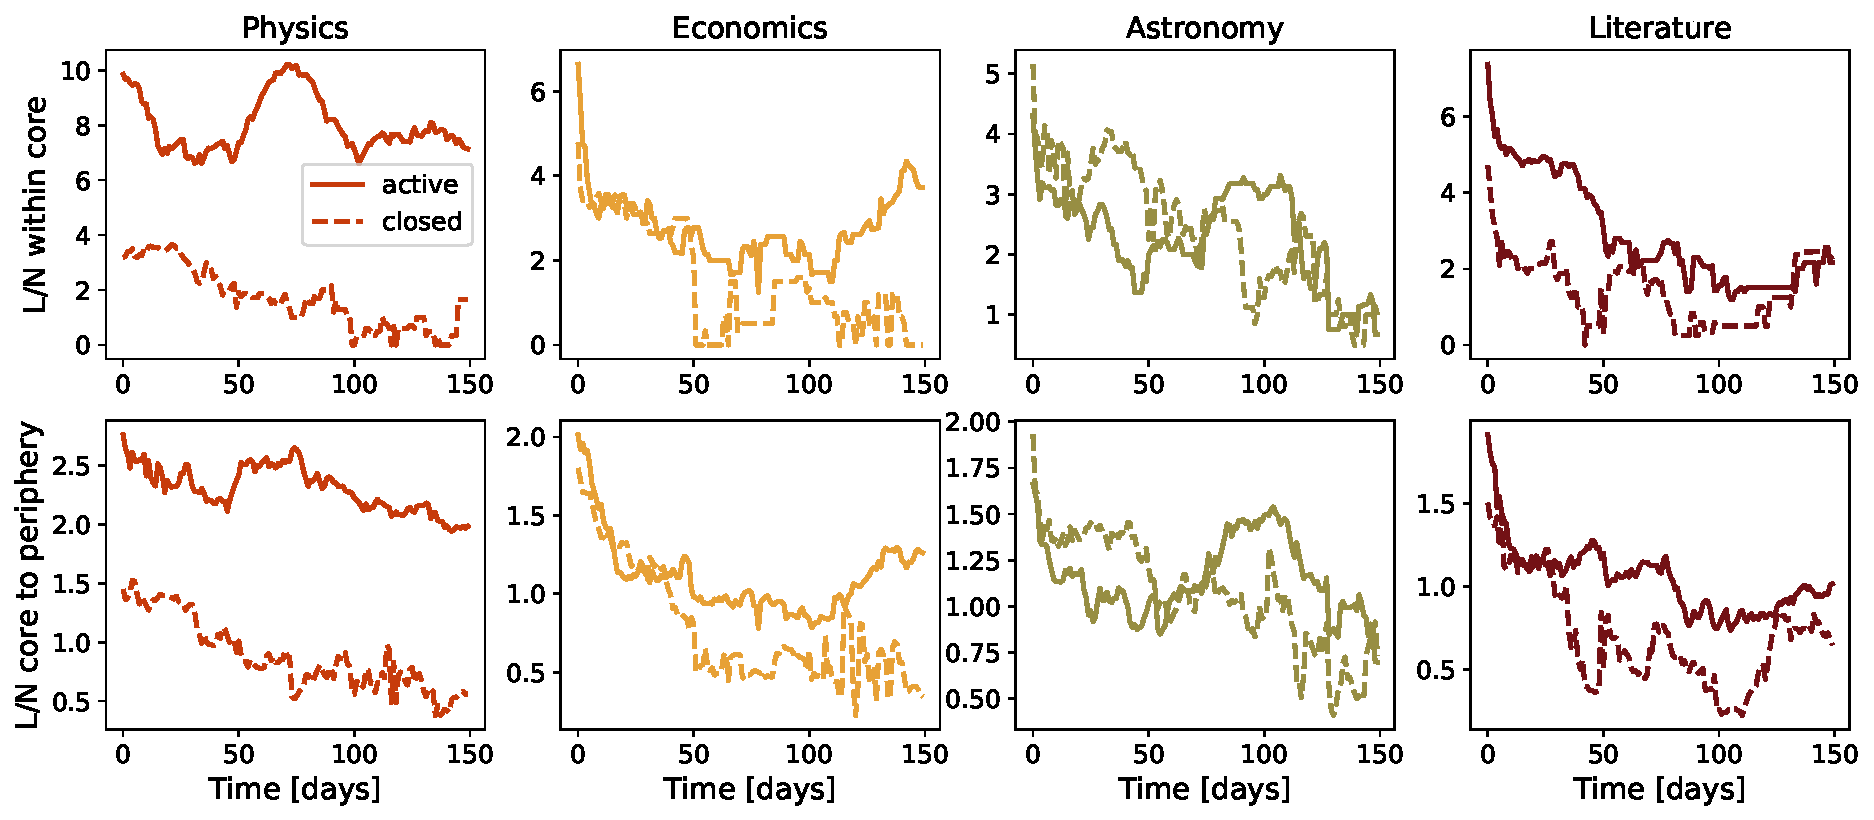
\includegraphics[width=\linewidth]{Figures/figures_SE/Fig5.pdf}
	\caption{Links per node in core and links per node between core and periphery.}
	\label{fig:links_per_node}
\end{figure}


\clearpage
\section{Dynamic reputation model}

Any dynamical trust or reputation model has to take into account distinct social and psychological attributes of these phenomena in order to estimate the value of any given trust metric \cite{duma2005dynamic}. First of all, the dynamics of trust is asymmetric, meaning that trust is easier to lose than to gain. As part of asymmetric dynamics, in order to make trust easier to loose the trust metric has to be sensitive to new experiences (recent activity or the absence of the activity of the agent), while still maintaining nontrivial influence of old behavior. The impact of new experiences has to be independent of
the total number of recorded or accumulated past interactions, making high levels of trust easy to lose. 
Finally, the trust metric has to detect and penalize both the sudden misbehavior and the possibly long term oscillatory behavior which deviates from community norms.

We estimate dynamic reputation of the Stack Exchange users using Dynamic Interaction Based Reputation Model (DIBRM) \cite{melnikovDynamicInteractionBasedReputation2018}. This model is based on the idea of dynamic reputation, which means that the reputation of users within the community changes continuously through time: it should rapidly decrease when there is no registered activity from the specific user in the community (reputation decay), and it should grow when frequent, constant interactions
and contributions to the community are detected. The highest growth of user's reputation is found through bursts of activity followed by short period of inactivity. 

In our implementation of the model, we do not distinguish between positive and negative interactions in the Stack Exchange communities. Therefore, we treat any interaction in the community (question, answer or comment) as potentially valuable contribution. In fact, evaluation criteria for Stack Exchange websites going through beta testing, described in SI, do not distinguish between positive and negative interactions.
The percentage of negative interactions in the communities we investigated was below 5\%, see Table 1 in SI. Filtering positive interactions would also require filtering out comments because they are not rated by the community, and that would eliminate a large portion of
direct interactions between the users of a community, which is essential for estimating their reputation.

In DIBRM, reputation value for each user of the community is estimated combining three different factors: 1) \textit{reputation growth} - the cumulative factor which represents the importance of users' activities; 2) \textit{reputation decay} - the forgetting factor which represents the continuous decrease of reputation due to inactivity; \textit{the activity period factor} - measuring the length of the period of time in which the change of reputation happened. In case of Stack Exchange communities, the forgetting factor has a literal meaning, as we can assume that past contributions provided by a user are being forgotten by active users as their attention is captured by more recent content.

In line with the the basic dichotomy of reputation dynamics, which revolves around the varying influence of past and recent behavior, DIBRM has two components: \textit{cumulative factor} - estimating the contribution of the most recent activities to the overall reputation of the user; \textit{forgetting factor} - estimating the weight of past behavior. Estimating the value of recent behavior starts with the definition of the parameter storing the basic value of a single interaction $I_{b_{n}}$. Cumulative factor $I_{c_{n}}$ then captures the additive effect of recent successive interactions. The reputational contribution $I_n$ of most recent interaction $n$ of any given user is estimated in the following way:

\begin{equation}\label{eq:ibn}
I_n = I_{b_{n}} + I_{c_{n}} = I_{b_{n}} (1+  \alpha  (1-\frac{1}{A_{n}+1}))
\end{equation}

Here, $\alpha$ is the weight of the cumulative part and $A_{n}$ is the number of sequential activities. If there is no interaction at $t_n$, this part of interactions has a value of 0. Important property of this component of dynamic reputation is the notion of sequential activities. Two successive interactions made by a user are considered sequential if the time between those two activities is less or equal to the time parameter $t_{a}$ which represents the time window of interaction. This time window represents maximum time spent by the user to make a meaningful contribution (post a question or answer or leave a comment).

\begin{equation}\label{eq:deltan}
\Delta_{n}=\frac{t_{n}-t_{n-1}}{t_{a}}
\end{equation}

If $\Delta_{n} < 1$ is less than one the number of sequential activities $A_{n}$ will increase by one, which means that the user is continuing to communicate frequently. On the other hand, large values $\Delta_{n}$ greatly increase the effect of the forgetting factor. This factor plays a major role in updating the total dynamic reputation of a user in each time step (after every recorded interaction):

\begin{equation}\label{eq:tn}
T_{n}=T_{n-1} \beta^{\Delta_{n}}+I_{n}
\end{equation}

Here, $\beta$ is the forgetting factor. In our implementation of the model, the trust is updated each day for every user irrespective of their activity status. Therefore, the decay itself is a combination of $\beta$ and $\Delta_n$: the more days pass without recorded interaction from a specific user, the more their reputation decays. Lower values of beta lead to faster decay of trust as shown on figure \ref{fig:paper_summary}.


%\subsection{Selection of dynamical reputation model parameters} \label{section:param}
One of the largest drawbacks of DIBRM is the parameter tuning problem. In previous applications of the model \cite{melnikovDynamicInteractionBasedReputation2018,yashkina2020} there was no single best set of parameter values for modeling dynamic reputation in Stack Exchange communities. For example, in \cite{yashkina2020} the best approximation of the official Stack Exchange reputation is obtained with $t_a =2, \beta = 1, \alpha = 1.4$ which means there is no active forgetting factor. In our application of DIBRM to SE communities we opted for a different set of parameter values. Details of parameter search and tuning are presented in SI.

For basic reputation contribution of a single interaction we selected $I_{bn} = 1$ and at the same time this is the threshold value of an active user. This value is intuitive as every interaction has initial contribution of +1 to user's reputation, although the previous works have used values of +2 and +4. Following the previous work and after examining the median/average time between subsequent interactions of the same user, we selected $t_a = 1$, which also means that reputation in our model will be updated every day during the time-window of the analysis, regardless of whether the user is active or not. To emphasize the bursts of activity and frequent recent interactions, cumulative factor has a larger value $\alpha = 2$. Finally, the most delicate parameter is the forgetting factor, which at the same time determines the weight of past interactions and the reputational punishment due to user inactivity. Here we need to select the value of parameter $\beta$ so we include the forgetting due to inactivity but not to penalize is too much. In Fig. A1 we show how different values of parameter $\beta$ influence the time needed for user's reputation to fall on value $I_{n}=1$ due to user's inactivity and value of dynamical reputation in the moment of the last activity. The higher the value of parameter $\beta$ and initial dynamical reputation of users, the longer time it takes for user's reputation to fall on baseline value. For parameter $\beta=0.9$ and $I_{n}=5$, user's reputation falls on value $I_{n}=1$ after less than 20 days, while this time is doubled for $\beta=0.96$. We see, that for higher values of parameter $\beta$ the time needed for $I_{n}$ to fall on value $1$ becomes longer, and that the the initial value of reputation becomes less important. 

Figure A2 in SI shows the difference between the number of users that had at least one activity in the window of 30 days and number of users with reputation higher than $1$ during the same period for different values of parameter $\beta$. The minimal difference between these two variables is observed for the values of $\beta$ between $0.94$ and $0.96$ for both live and closed communities. Since we want to compare communities, we select $\beta = 0.96$ after verifying that this level of reputational decay does not reduce the number of active users (based on their dynamic reputation) below the actual number of users who have been active (interacted with the community) in the time window of 30 days. 

To summarize, our model of dynamical reputation has three parameters: 1) basic reputation contribution $I_{bn}=1$; 2) cumulative factor $\alpha=2$; 3) forgetting factor $\beta=0.96$. The selected values of parameters are used for measuring dynamical reputation of user in all four pair SE communities. Given these values of parameters, the minimal reputation achieved by the user immediately after they have made an interaction in the SE community is $1$. This reputation will decay below $1$ if the user does not perform another interaction within the one-day time window. For any user in a community, when their reputation drops below $1$, we consider this user inactive which means that the user at that time is not "visible" in the community and their past contributions at that time are unlikely to impact other users. The number of active users and mean user reputation for different Stack Exchange communities are shown in Fig. \ref{fig:dr6panel}.

\begin{figure}
	%%% 6 panels
	%%% columns: Total rep., Mean rep., Number of Active Users
	%%% rows 1: Physics. Theo. Physics, Econ. Beta, Econ. A51
	%%% rows 2: Astro Beta, Astro A51, Lit Beta, Lit A51
	\centering
	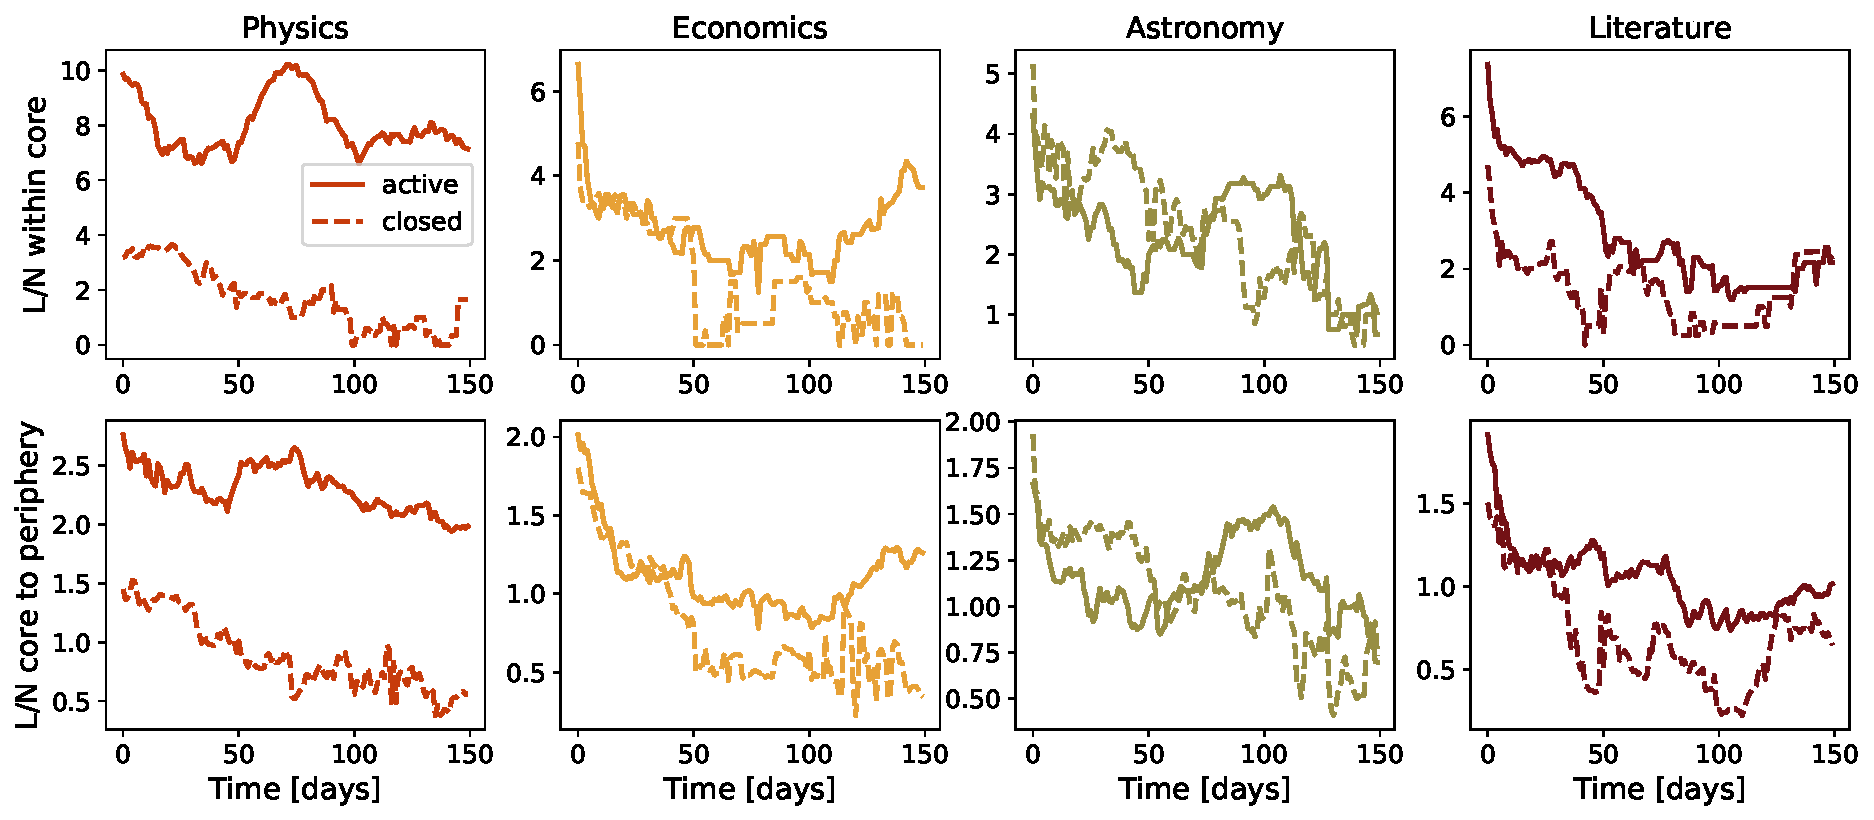
\includegraphics[width=\linewidth]{Figures/figures_SE/Fig5.pdf}
	\caption{Dynamic Reputation on the four pairs of Stack Exchange websites: Astronomy, Literature, Economics,  Physics and Theoretical Physics.}
	\label{fig:dr6panel}
\end{figure}


\subsection{Dynamic reputation of users within the network of interactions}

\begin{figure}
	\centering
	%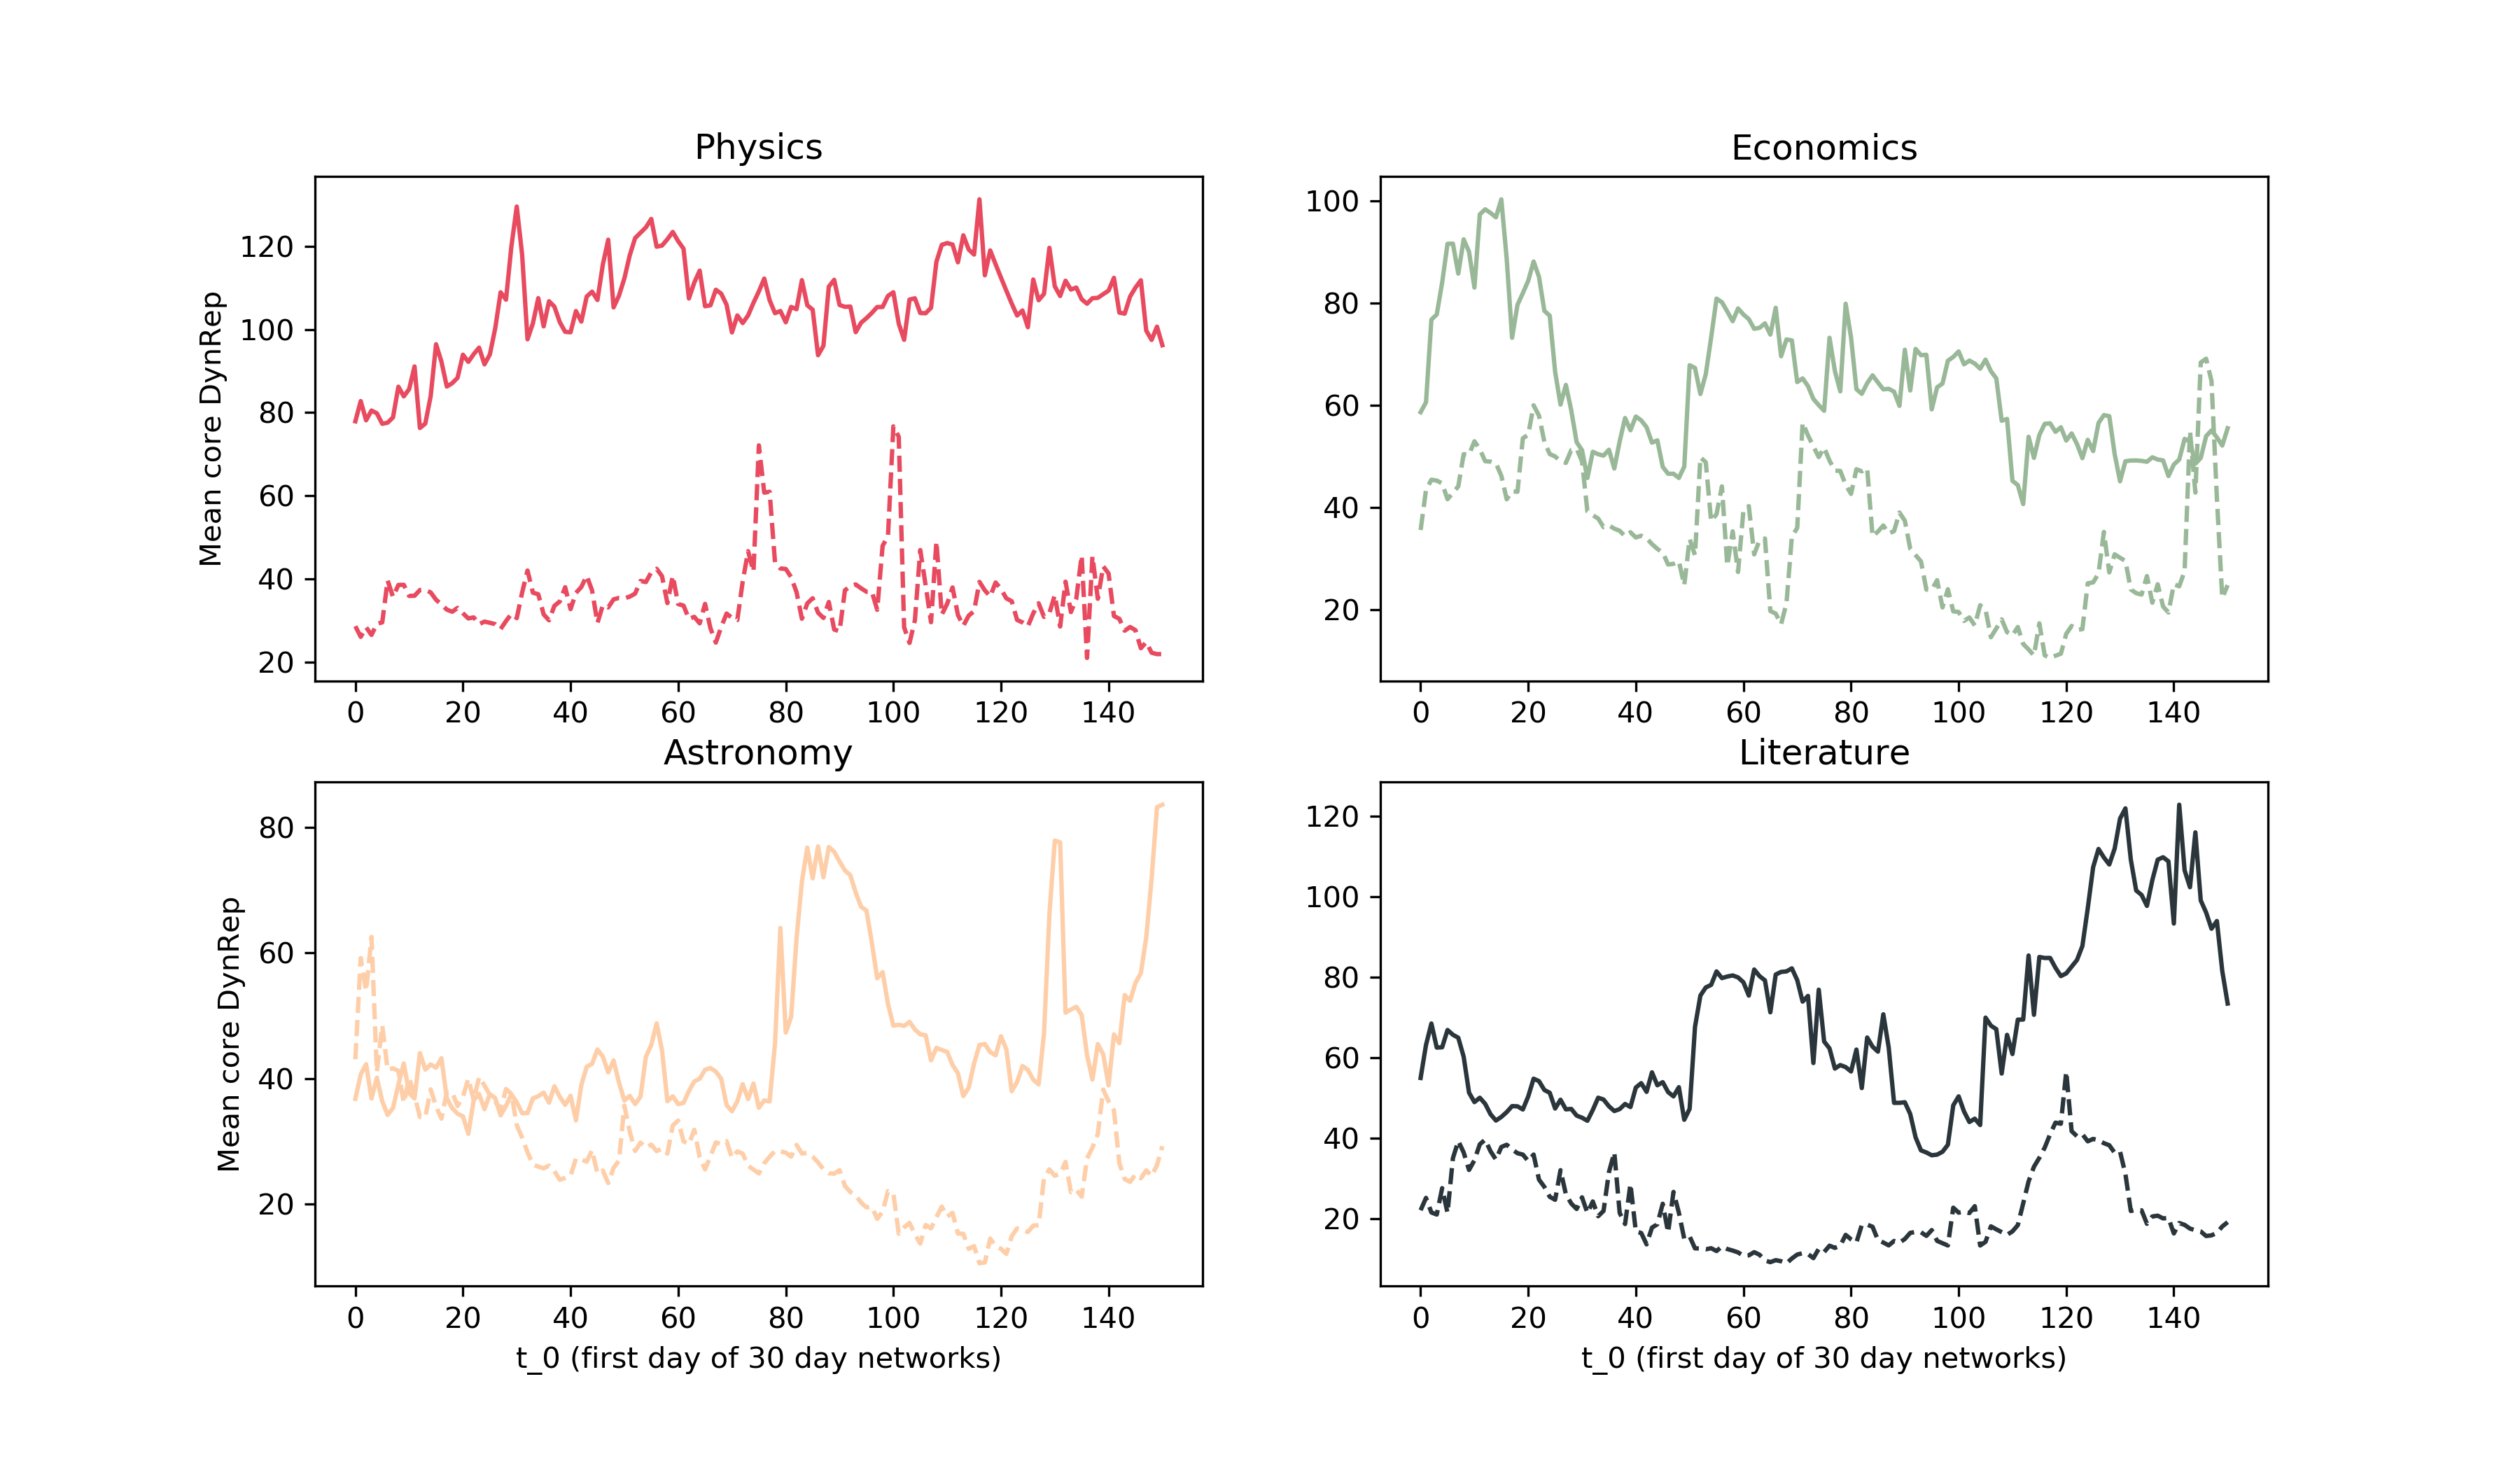
\includegraphics[width=\linewidth]{figures/Mean_core_dyn_rep.png}
	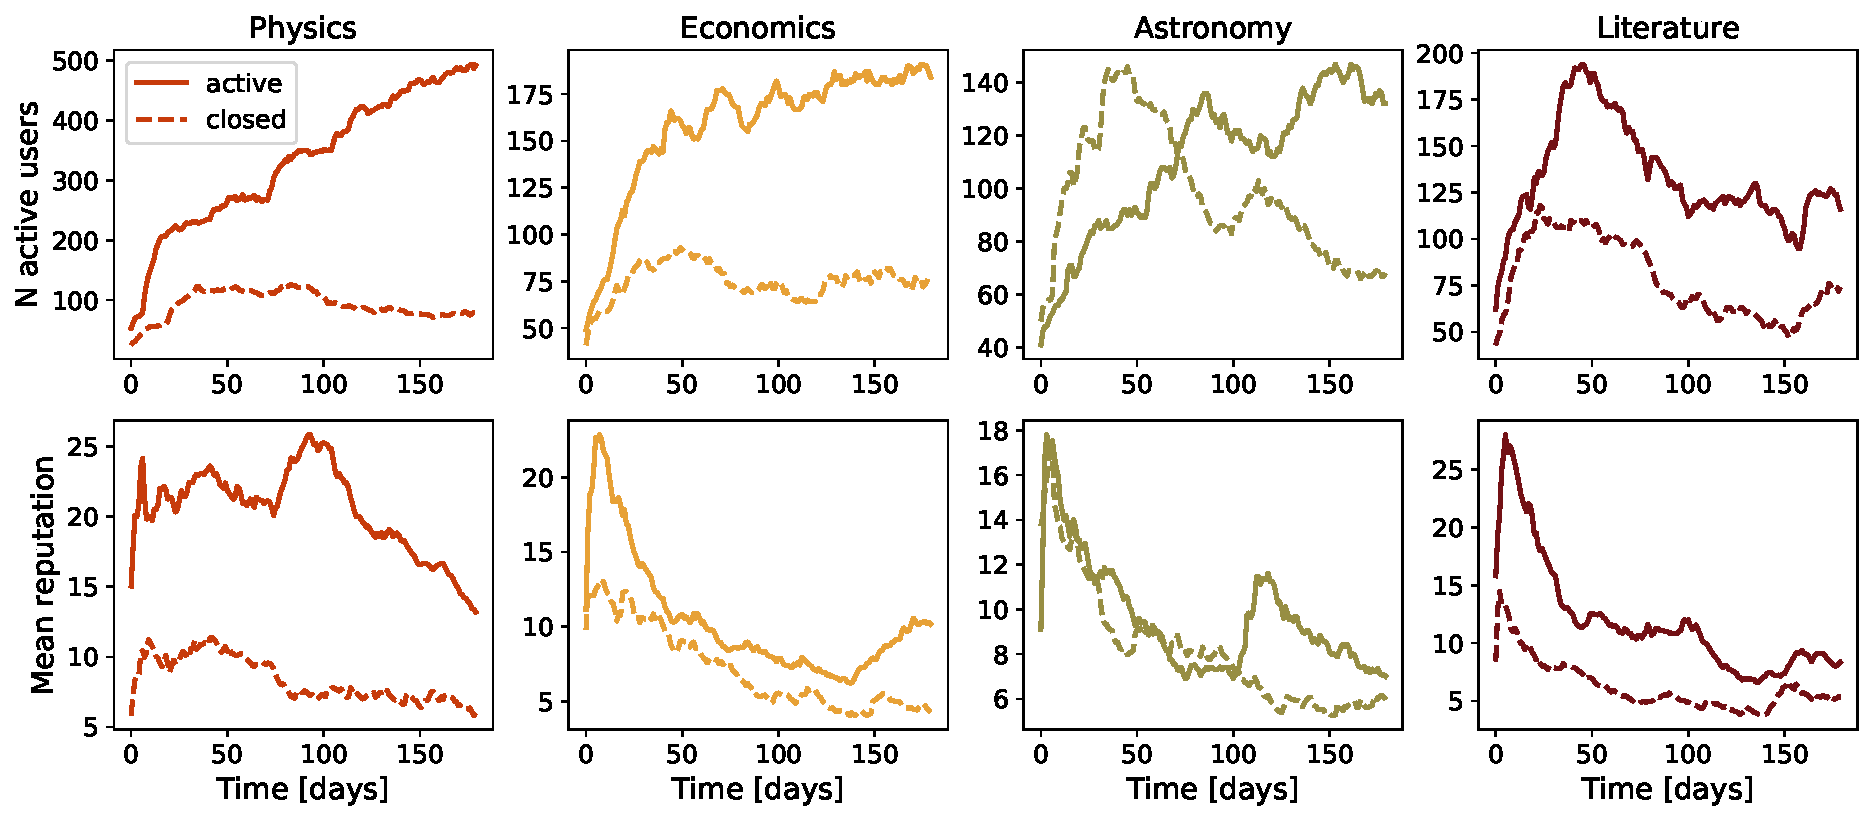
\includegraphics[width=\linewidth]{Figures/figures_SE/Fig4.pdf}
	\caption{Dynamical reputation within core.}
	\label{fig:dr_core}
\end{figure}

Examined network properties suggest that there are structural differences between active and closed communities. Active communities have higher and more stable local cohesiveness compared to their closed counterparts. The overlap of the set of nodes in the core for active communities shows a significant overlap even for distant subnetworks, meaning that the membership of the core in active communities is more stable.

To further explore the differences between active and closed communities, we focus on dynamical reputation which is our proxy for collective trust in these communities. We investigate whether and how core-periphery structure is related to collective trust in the network. Figure \ref{fig:dr_core} shows the mean dynamical reputation in the core of active and closed communities and its evolution during the observation period. There are clear differences between active and closed communities when it comes to dynamical reputation. The mean dynamical reputation of core users is always higher in active communities than in closed. As expected, the largest difference is observed between Physics and Theoretical Physics community. The difference between active communities which are still in the beta phase and their closed counterparts is not as prominent, however, the active communities have higher mean dynamical reputation especially in the later phase of community life. The only difference in the pattern is observed for astronomy communities at the early phase of their life, when closed community has a higher value of dynamical reputation than active community. This is in line with similar patterns in the evolution of mean clustering and core-periphery structure. 

By definition, the core consists of very active individuals and thus we expect higher total dynamical reputation of users in the core in comparison to the the total reputation of users belonging to subnetworks periphery. Figure A12 shows the ratio between the total reputation of core and periphery for closed and active communities and its evolution. The ratio between total reputation of core and periphery in Physics is always higher than in the Theoretical physics community. Similar pattern can be observed for literature communities, although the difference is not as clear as in the case of physics. Ratio of total dynamical reputation between core and periphery is higher for closed community than active one on the economics topic in the early days of community life. However, in the later stage of their lives this ratio becomes higher for active communities. Communities around astronomy topic deviate from this pattern, which once again shows the specificity of these communities. 

To complete the description of the evolution of dynamic reputation active and closed communities, we examine the evolution of Gini index of dynamical reputation in the whole network which is shown in Fig. A5 in Supplementary Information. The Gini index is always higher for active communities than for closed ones, especially for later times in observation period. Only pattern of Astronomy communities deviates from the pattern observed for other three pairs during the early days. These results indicate that the dynamical reputation is distributed in the population more unequally in the active than in closed communities. The evolution of assortativity coefficient that measures correlations between dynamical reputation of connected users in the subnetworks, shown in Fig. A6, shows that networks are disassortative for the largest part of the observation period. These results suggest that users with high dynamical reputation have tendency to connect with users with low value of dynamical reputation. 


In Figure~\ref{fig:dyn_rep_coreper} we show mean user reputation in core and in periphery over time (30 day sliding windows as before). We see that the mean user reputation in core is greater in the currently active sites (solid lines, top panels) than in their closed pairs (dashed lines). In the bottom panels, we see that the mean reputation on the network periphery has substantially lower values, and the difference between active and closed sites is less pronounced. 

For reference in Fig~\ref{fig:core_size} we show core sizes in all sites. We show these in absolute numbers (total number of nodes) and as a fraction of network size through time.



\subsection{Dynamic reputation - $\beta$ parameter}

Our implementation of dynamic reputation model was based on $\beta = 0.96$. There are several reasons for selecting this value.

In Dynamic reputation model, the $\beta$ parameter controls the strength of the forgetting fator of the model.  The value of this parameter should reflect the core feature of the reputational systems and make reputation easier to loose. Due to user's inactivity, any level of reputation will eventually decay to below 1. Dependence of time needed for reputation to drop below this level and the $\beta$ parameter, as well as reputation before inactivity is shown on Figure~\ref{fig:betadelta}. Here $I_n$ is equal to the raw number of interactions in the community without forgetting or cumulative factor at work.

\begin{figure}[h!]
	\centering
	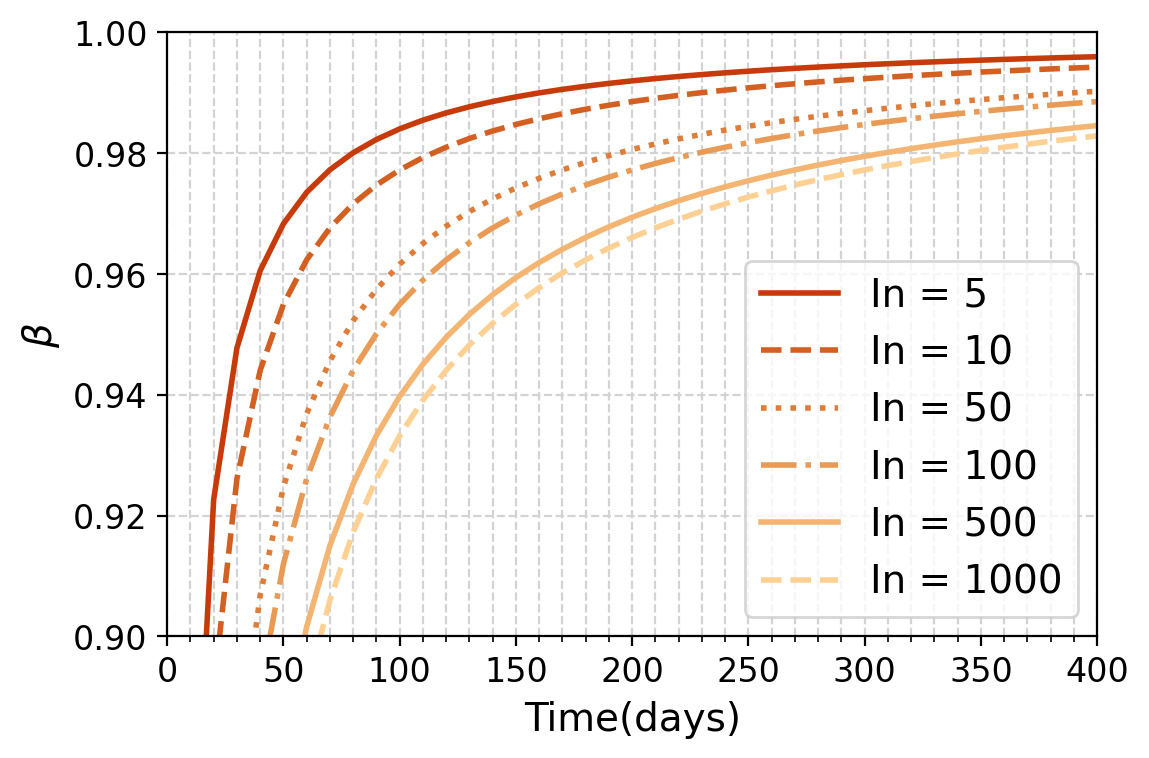
\includegraphics[width=0.5\linewidth]{Figures/FigA1.png}
	% REMOVE 'SLOWER' FROM THE PLOT TITLE > zamenjeno i formulu sam prebacila u caption
	\caption{Dependence of parameter $\beta$ and number of days $\Delta$ needed for reputation $I_n$ to drop to $I_{n_0} = 1$. Dependence of parameter $\beta$ and number of days when reputation due inactivity decreases from $I_n$ to $I_0$ is given as  $\beta = (\frac{I_{n0}}{I_{n}})^{(1/\Delta)}$ }
	\label{fig:betadelta}
\end{figure}

For $\beta$ values below 0.96, the decay is fast and within two to four months of inactivity even high values of reputation are reduced below the threshold. On the other hand, with $\beta$ values the decay proces is more differentiated and high reputation becomes harder to loose, surviving up to a year of inactivity. For $\beta$ equal to 0.96, it takes a month for reputation based on 5 interactions to decay and around five months for high reputation based on 500 or 1000 interactions to decay below the threshold.

\textbf{30 days sliding window} We compared the number of users with estimated reputation higher than 1 for different parameters $\beta$ and concluded that $\beta$ close to $0.96$ approximates the number of users with recorded interactions in a given 30 days sliding window. For each pair of communities we calculated number of users with at least one interactions in every 30 days sliding window and then we estimated several times series expressing the number of users with reputation higher than 1 for fixed $\beta$. Then we calculated the root mean square error (RMSE) between those time series for the first 200 days. Values of RMSE are shown on Figure~\ref{fig:rmse}. For each community, we can find parameter $\beta$ that minimizes RMSE. Although $\beta$ does not have a unique value across communities, it varies between 0.95 and 0.96. 
%We should notice that taking different time period, for example, the first 90 days, we can get different optimal values of betta, but they'll probably take values between 0.95 and 0.96 (I can test it). 


\begin{figure}[h!]
	\centering
	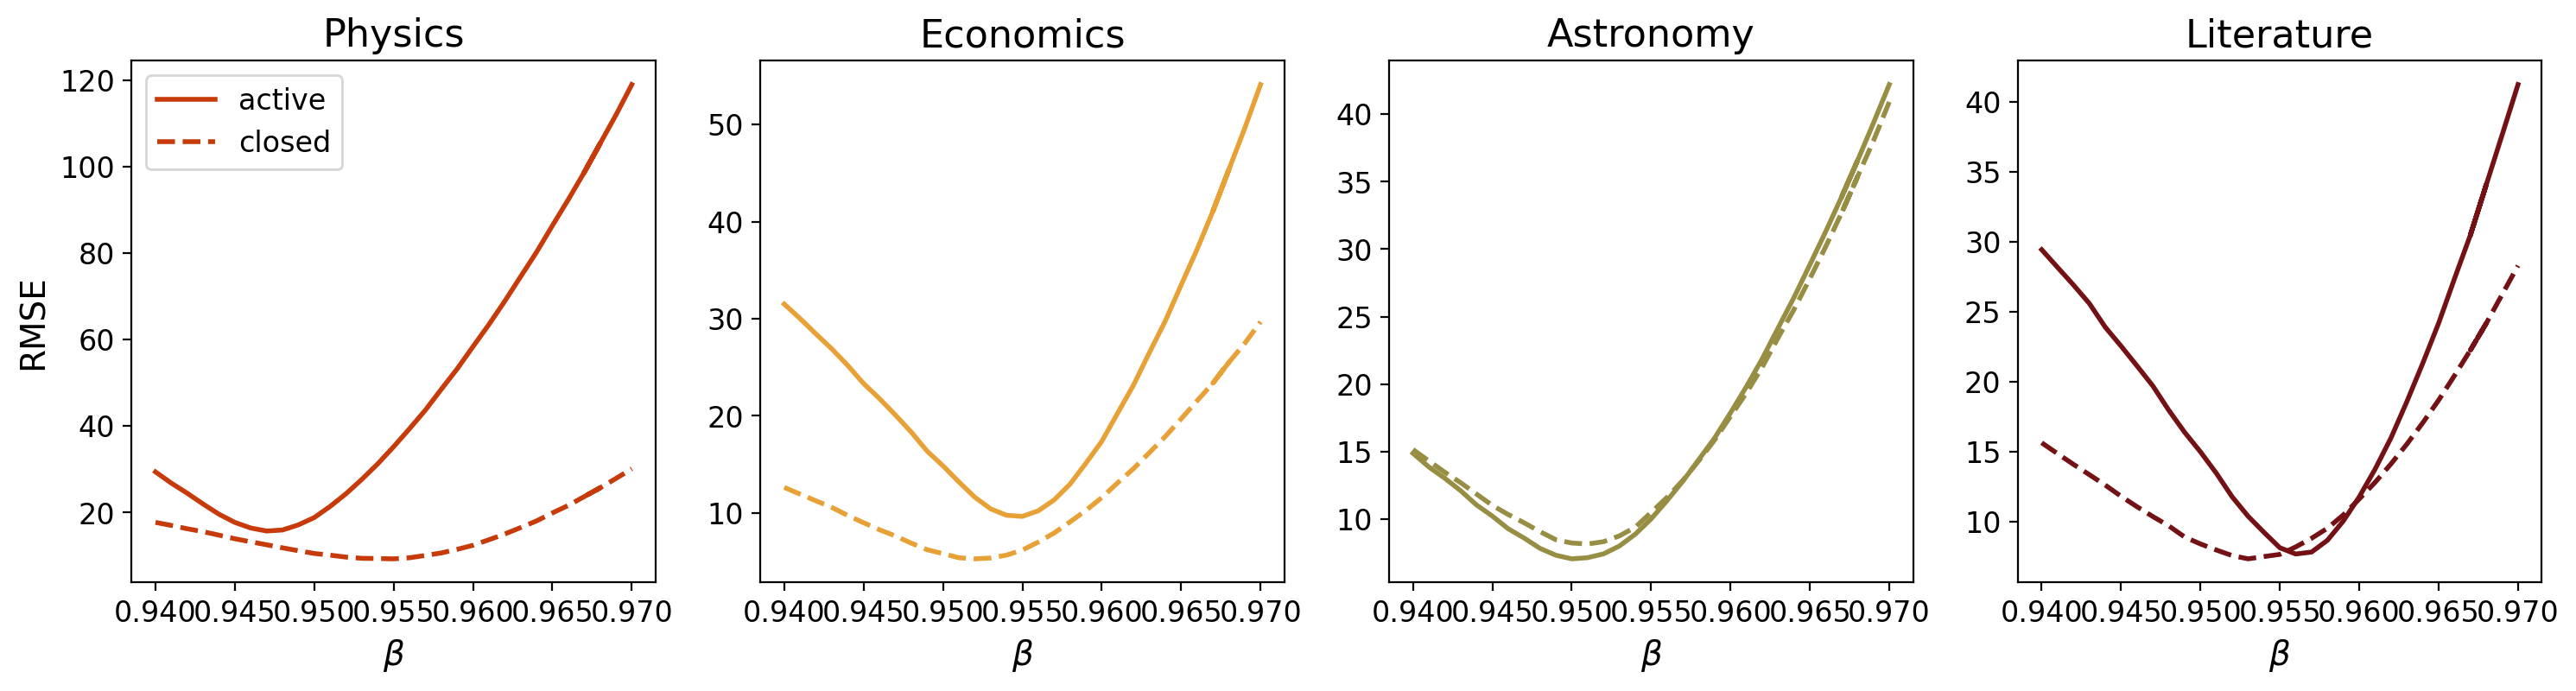
\includegraphics[width=\linewidth]{Figures/FigA2.png}
	\caption{RMSE between number of active users in sliding window of 30 days and number of users with reputation $>1$ for  $0.94< \beta <0.97$ with step $0.001$. }
	\label{fig:rmse}
\end{figure}

Figure \ref{fig:nusers} shows comparison between number of users in 30 days sliding window, number of users for these optimal values $\beta = 0.954$ and $\beta =0.96$. For $\beta = 0.96$ we observe that in most communities estimated number of active users consistently slightly higher than the actual number of users which have made at least one interaction in that sliding window. This means that dynamic reputation model in some cases overestimates the reputation of the user, but far more important is that it never understimates the real number of active users. Since we base our calculations of total and average reputation within the community only on users whose reputation is higher than the threshold this is important as no active users are disregarded by the model due to the value of the decay parameter.

\begin{figure}[h!]
	\centering
	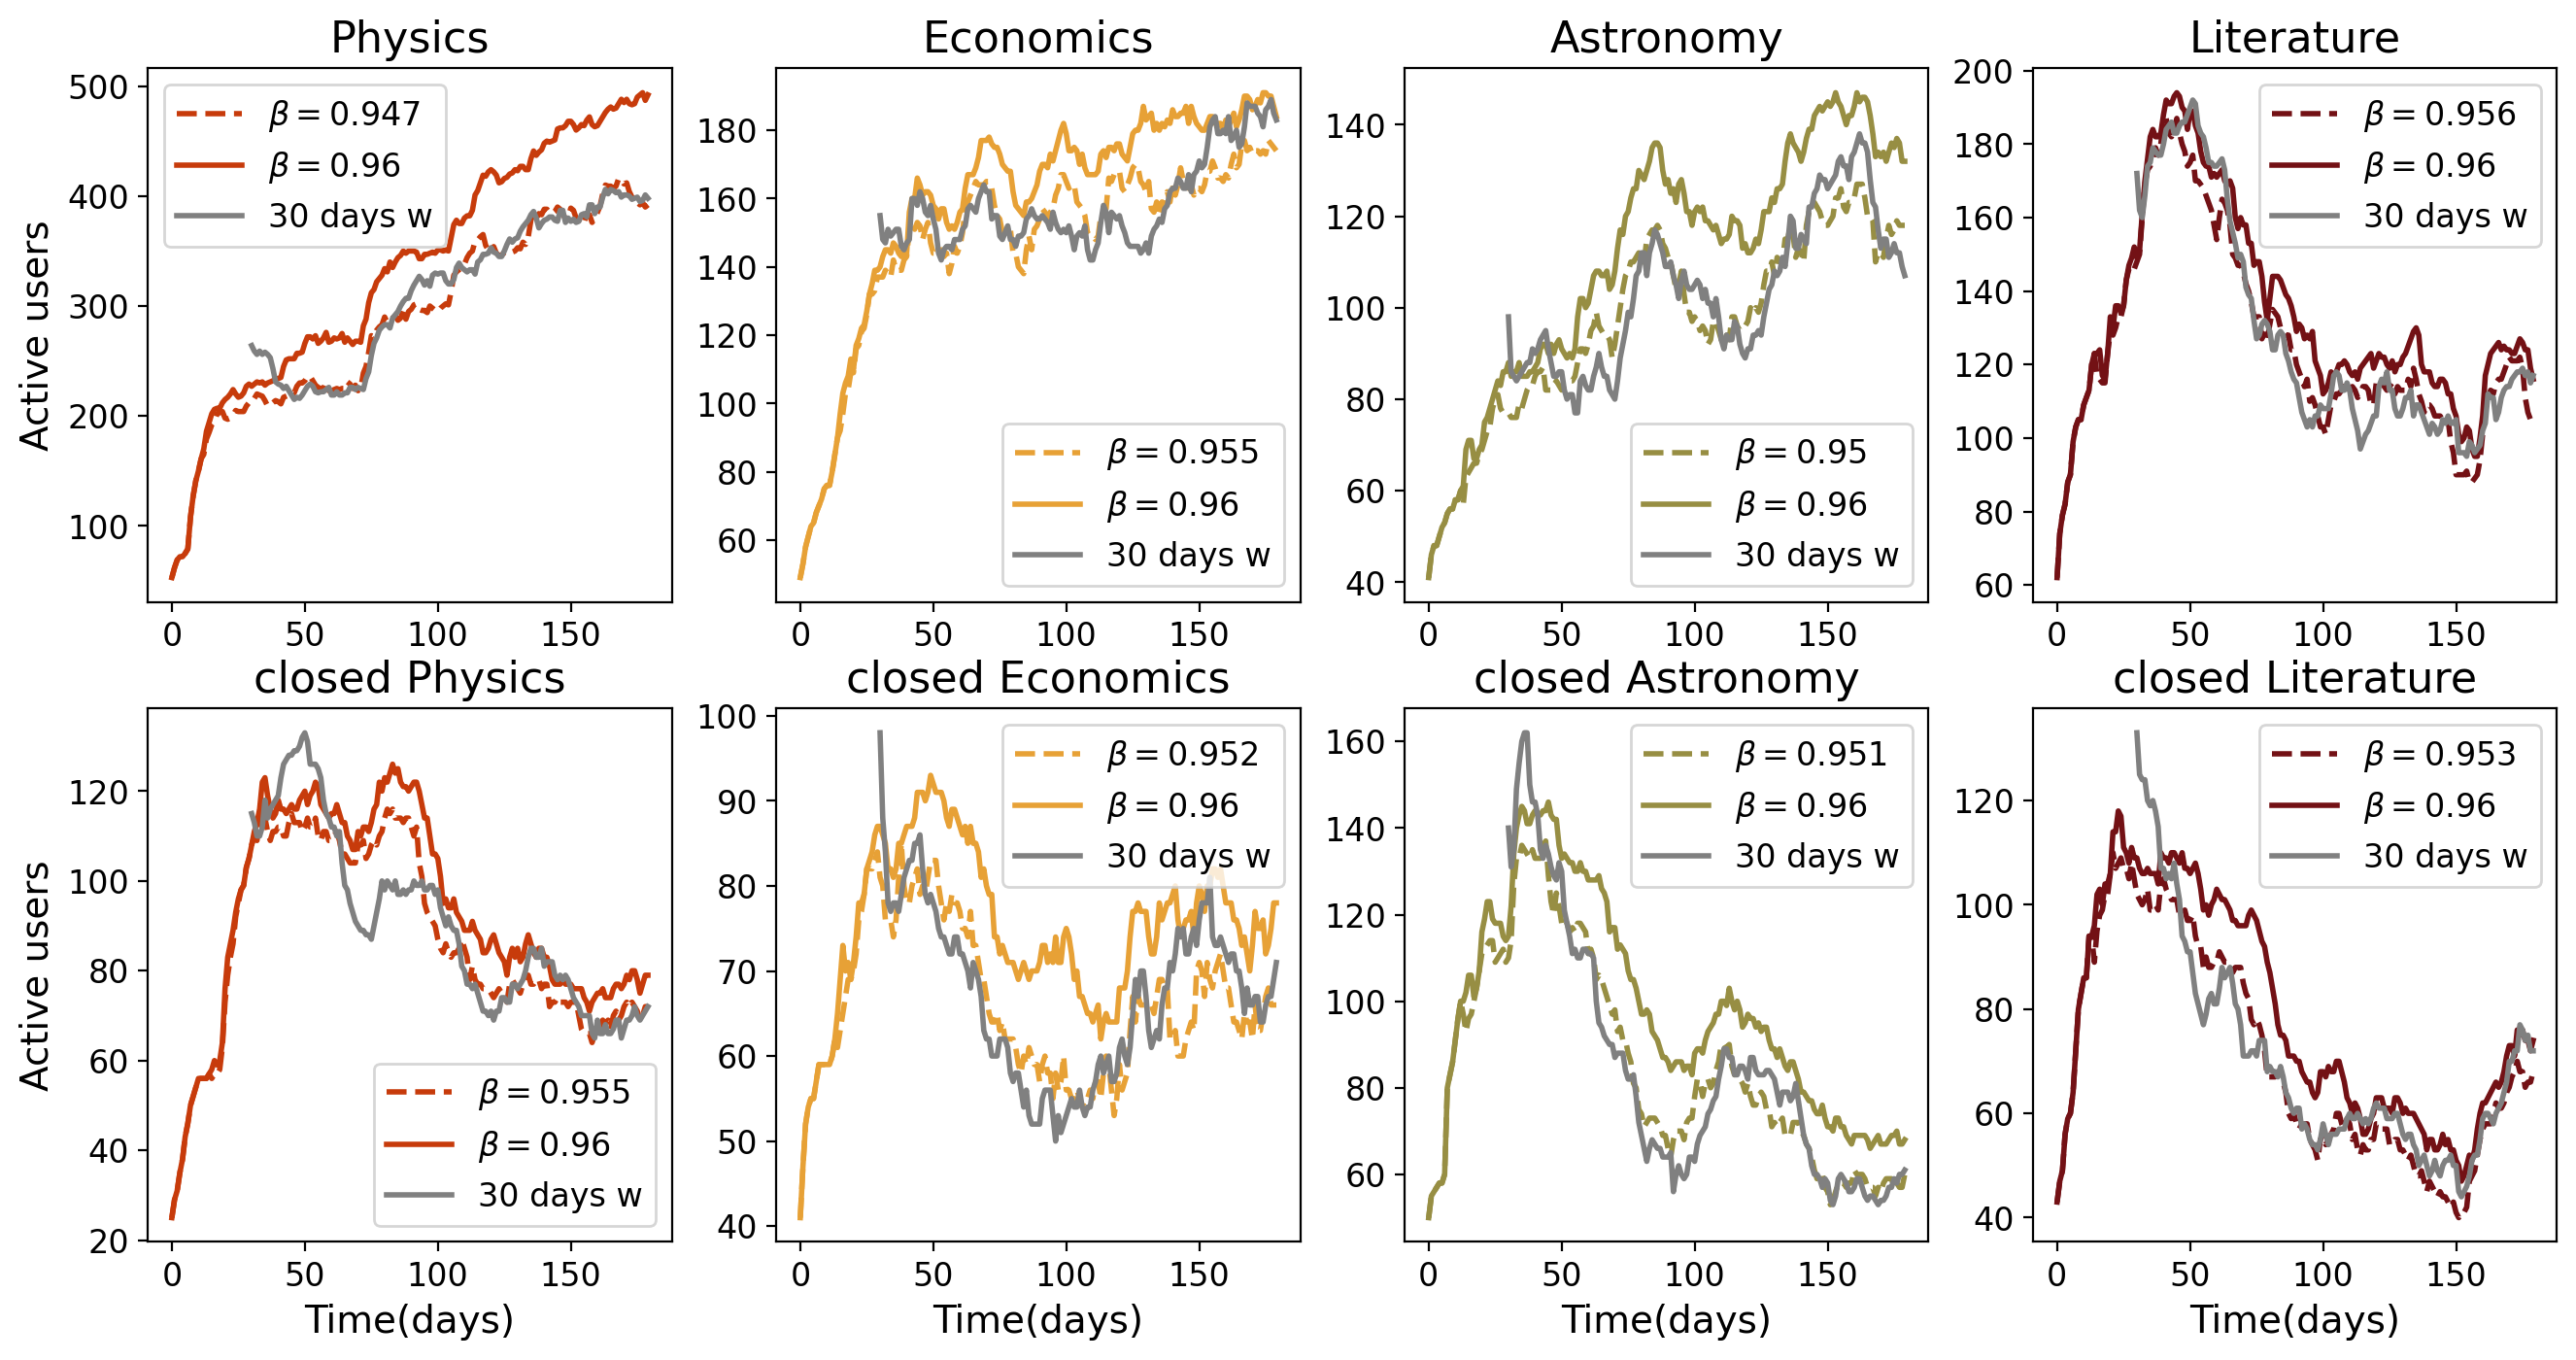
\includegraphics[width=\linewidth]{Figures/FigA3.png}
	\caption{Number of active users in a sliding window of 30 days and number of users with dynamic reputation higher than 1 for $\beta=0.954$ and $\beta=0.96 $ which provide the best fit to the number of users in 30 days sub-networks for each community}
	\label{fig:nusers}
\end{figure}

Finally, it's imporant that our dynamic reptuation captures the trend of long-term user activity. In Figure~\ref{fig:active-users} solid lines show the time series of estimated dynamic reputation for $\beta = 0.96$ while dashed lines show the number of users who were active in a given sliding window and continued to be active in the next one. Although the total estimated number of active users is expectedly higher, two time series follow similar trends in different communities.

\begin{figure}[h!]
	\centering
	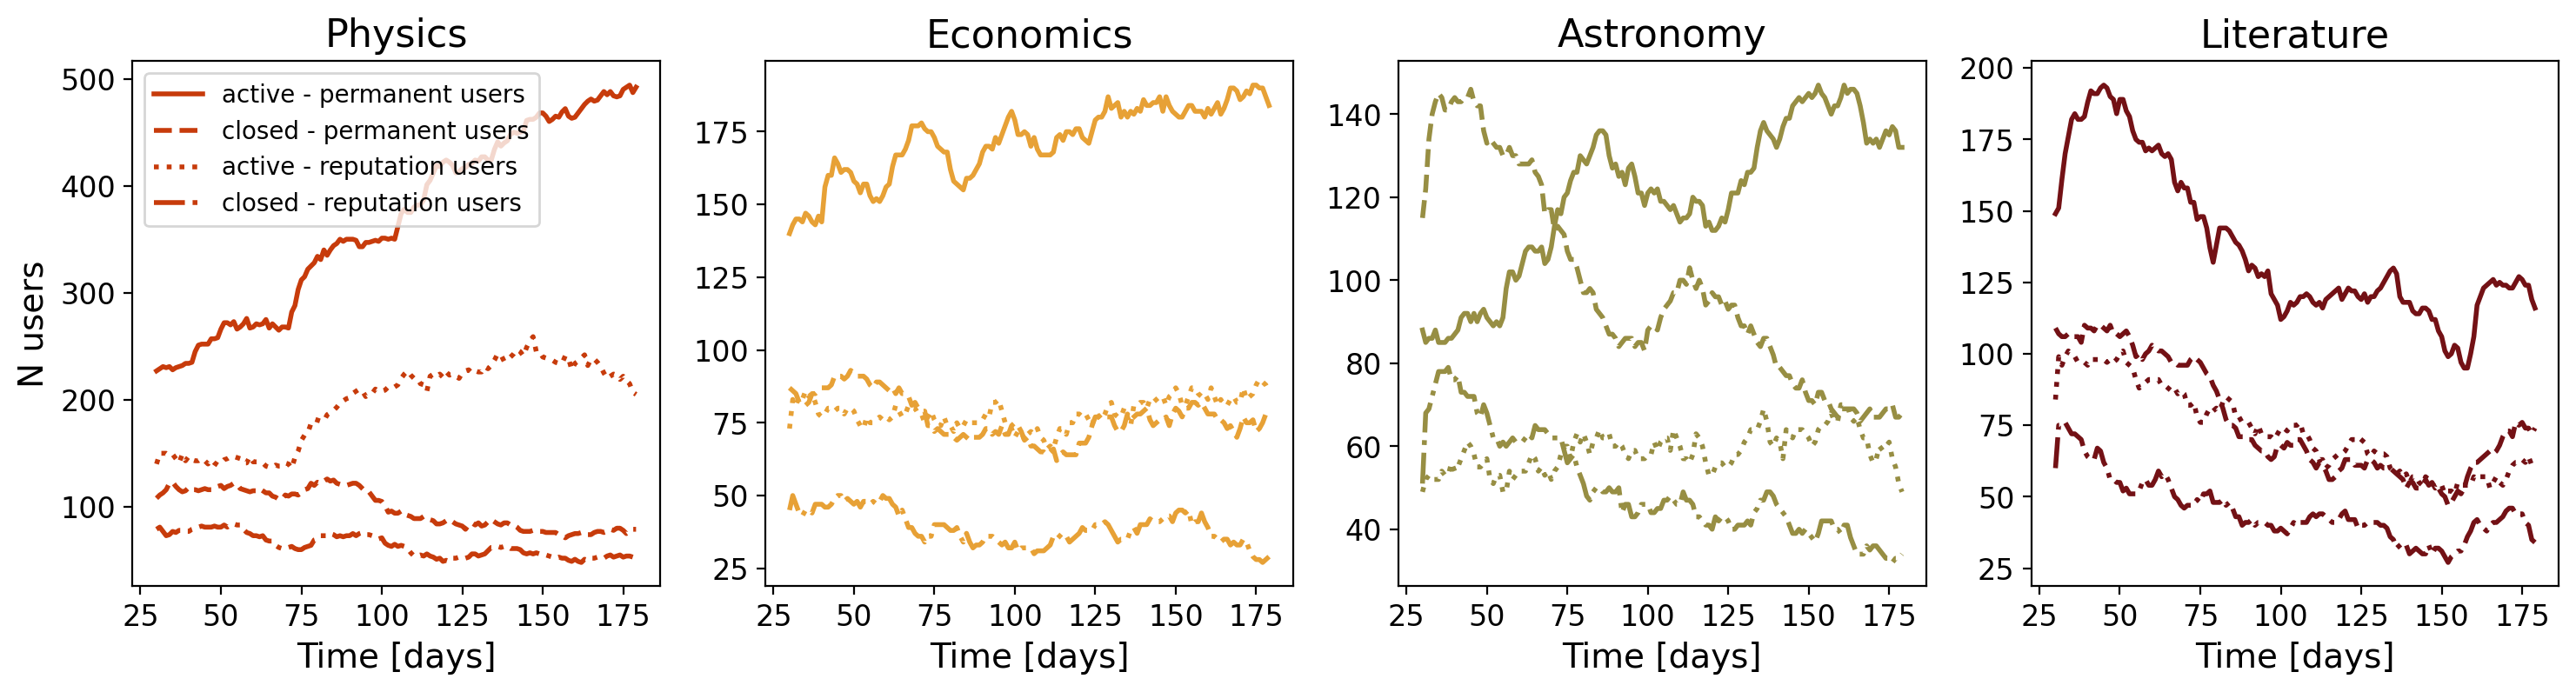
\includegraphics[width=1\linewidth]{Figures/FigA4.png}
	\caption{Solid lines represent number of users with dynamic reputation higher than 1 for $\beta=0.96$ while dashed lines are number of users within 30 days sliding window who were active and remained to be active. Blue lines are beta, while red lines are area51 communities.}
	\label{fig:active-users}
\end{figure}
\clearpage


\textbf{Gini coefficient}
Besides the number of active users (who at given moment of observation have reputation higher than the threshold) and the population mean value of dynamical reptuation, we have investigated in more details the distribution of dynamical reputation within discussed communities. We have observed that the distributions are often skewed which prompted us to compare the communities in terms of their Gini coefficient. The gini coefficient is a simple measure that shows us the degree of reputation inequality within the community. We calculate the value based on the dynamic reputation values of users at every time step (day) and report he values in Fig.~\ref{fig:dynrep-gini}. We see that all communities (both still active and closed ones) have gini coeffiecinet values higher than $0.5$ throughout first six month period. Interestingly, except in the case of Astronomy, currently active communities had higher reputation inequality every day during first six month period. As in many other measures, in the case of astronomy, closed community started as more unequal one (signalled by higher gini coef values), but after around two months the situation changed. 
\begin{figure}[h!]
	\centering
	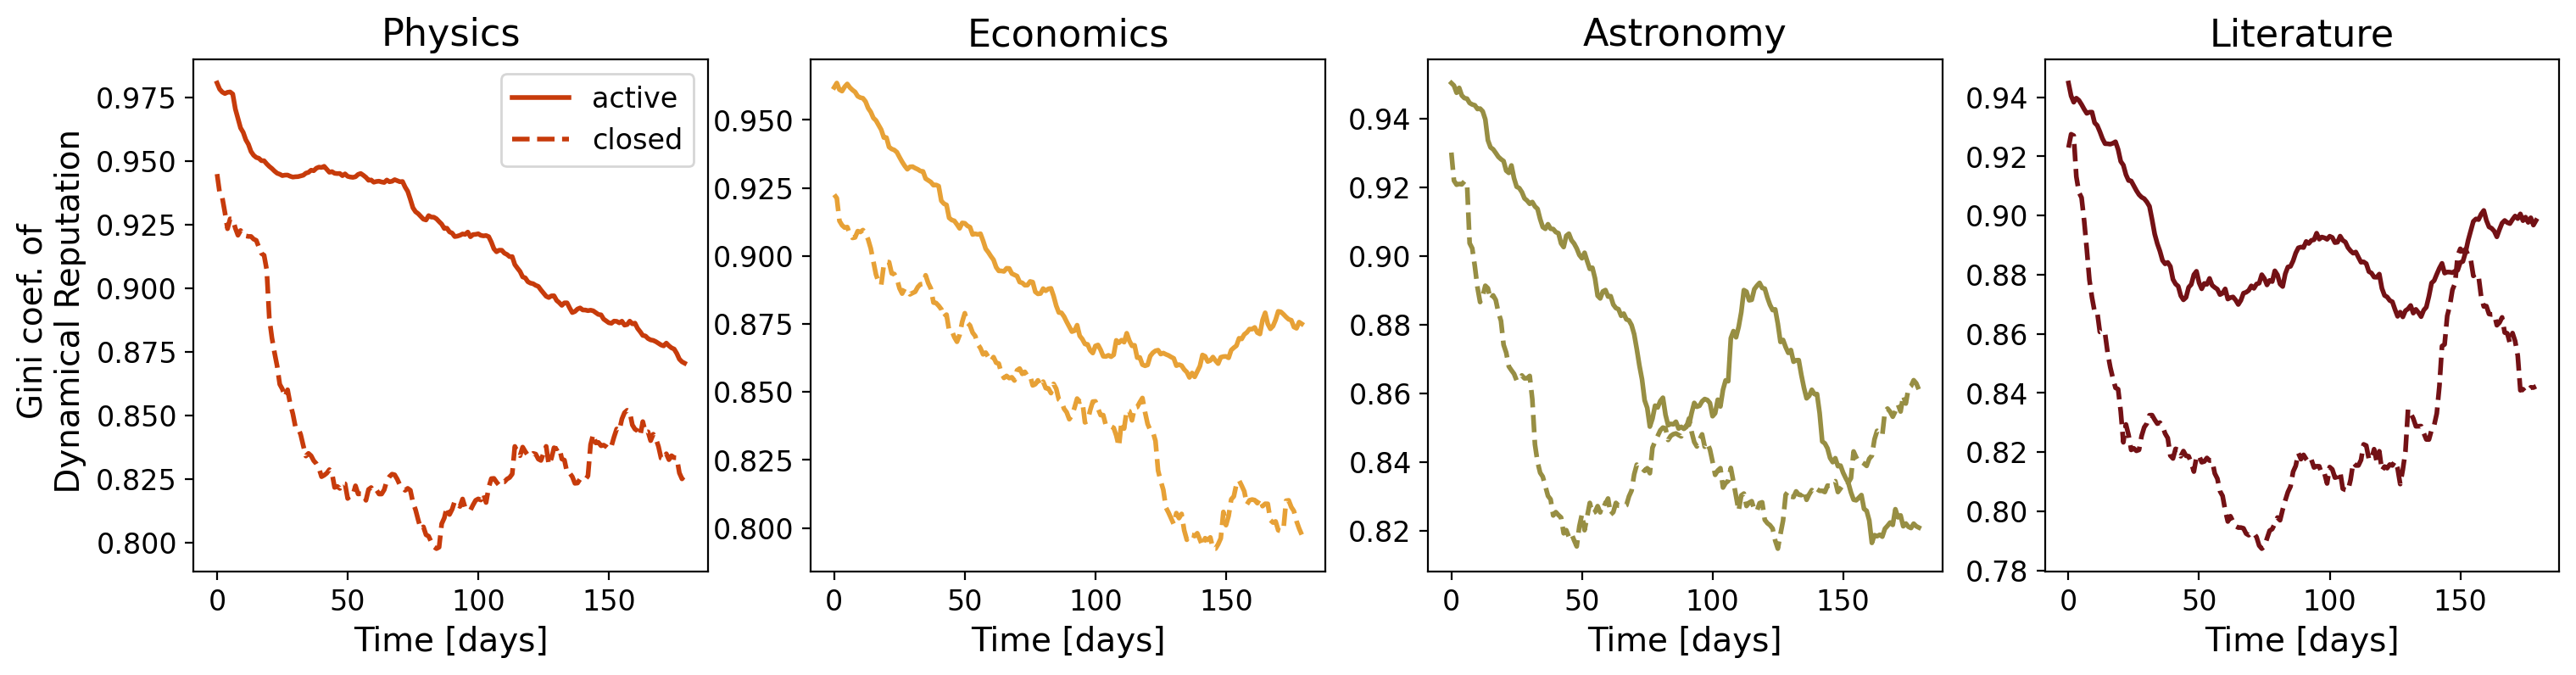
\includegraphics[width=1\linewidth]{Figures/FigA5.png}
	\caption{Gini index of dynamic reputation within population\textbf{Podsetnik da i ova slika treba da ide do 180 dana}}
	\label{fig:dynrep-gini}
\end{figure}

\subsection{Dynamic reputation in the network of interactions}
In the few figures below, we investigate whether users' dynamic reputation is related with users' position within the network.

\textbf{Dynamic Reputation assortativity}

We first look at user interaction patters, e.g. we investigate whether users connect with others of similar or different reputation (positive/negative assortativity). We operationalize this by measuring assortativity of dynamic reputation on interaction network. Practically this is a meassure of correlation between dynamic reputation of users who are linked in the interaction network. These results are shown in Fig.~\ref{fig:dyn_rep_assort}. We look at 30 day unweighted undirected networks of interactions (questions, answers and comments) and calculate assortativity by using users' reputation on the last day of observed time window. We see small values of assortativity that are mostly negative, signaling weak correlations between reputation levels of interacting users. The fact that the values are mostly negative are expected, users of different dynamic reputation interact, e.g. active, high reputation users respond to the questions of new, less reputable users. Exceptions are closed astronomy and literature sites that occasionally had positive assortativity values, signaling existence of links between users of similar reputation levels.
\begin{figure}[h!]
	\centering
	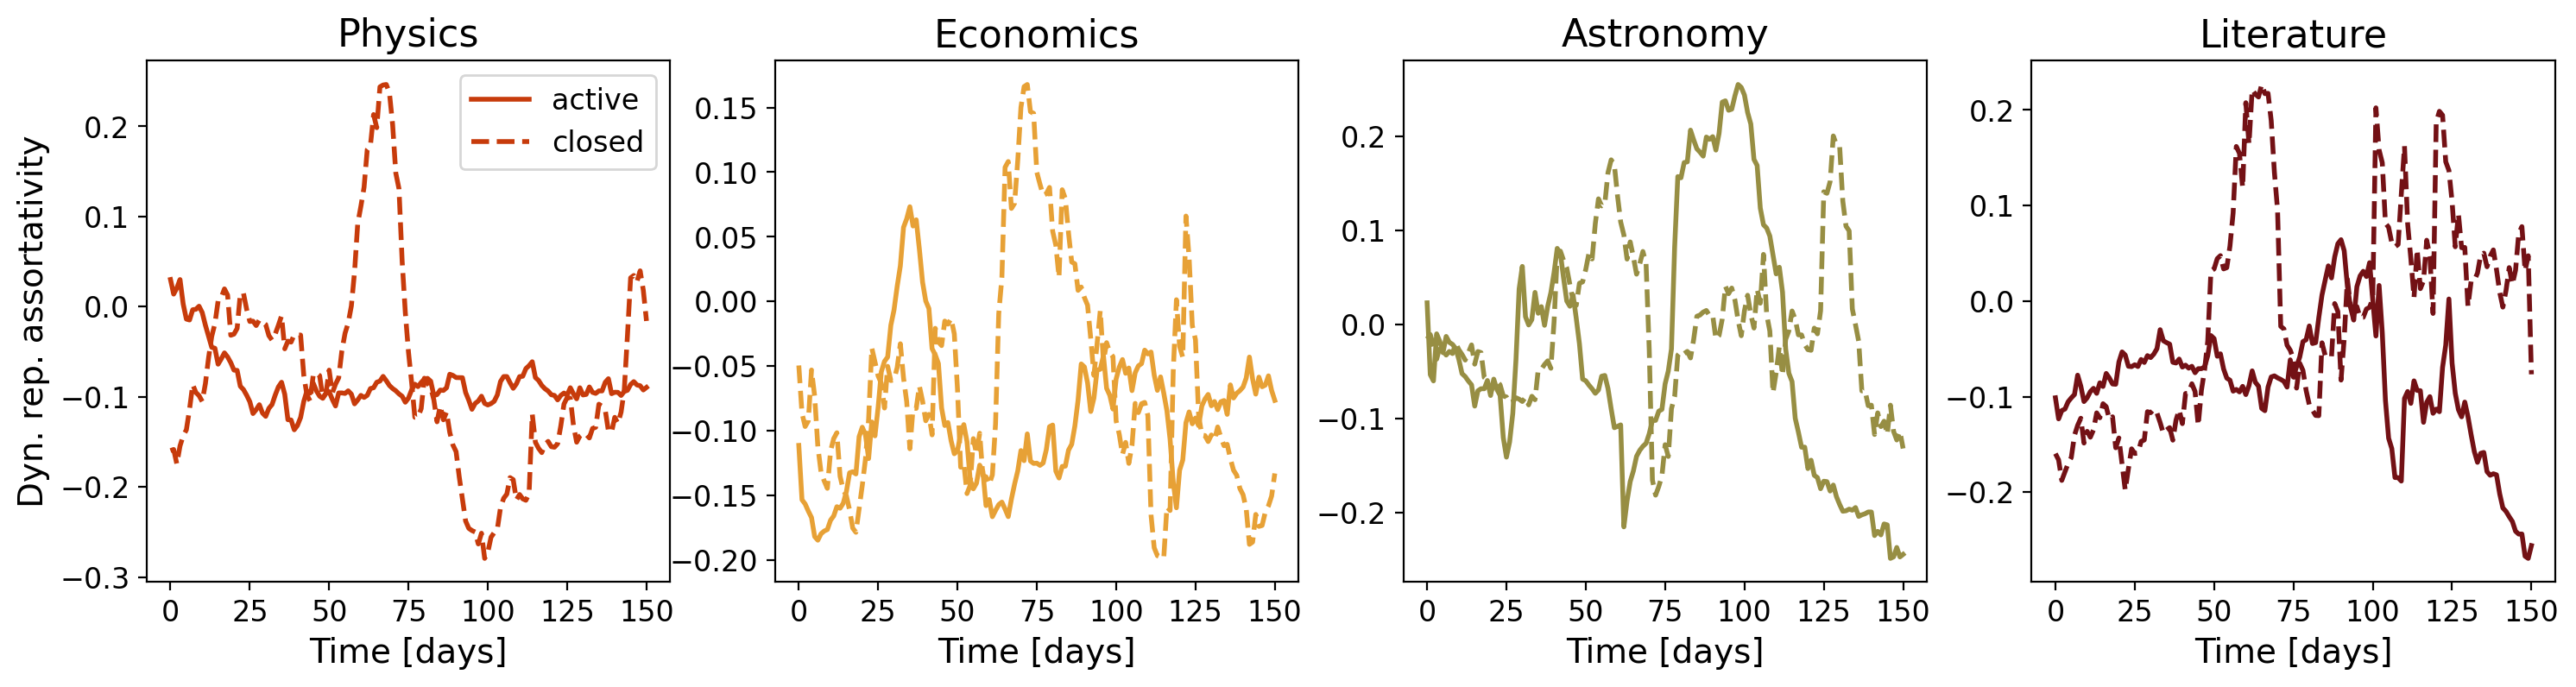
\includegraphics[width=1\linewidth]{Figures/FigA6.png}
	\caption{Dynamic Reputation assortativity in the network of interactions (questions, answers, comments, unweighted, undirected network). Solid lines - active sites; dashed lines - closed sites.}
	\label{fig:dyn_rep_assort}
\end{figure}
%% posto se ovo isto gleda na mrezama mozda moze u isti section sa ova dva grafika
\\~\\
\textbf{DynRep \& Degree}
% dodacu samo korelacije kroz vreme za sad stoji samo placeholder za sliku i opis
\textbf{DynRep \& BC}
% dodacu samo korelacije kroz vreme

We continue to investigate whether the user's reputation correlates with typical network centrality measures calculated at user's node in the interaction network. As previously, we compare node's centrality in the 30 day network with the node's dynamic reputation on the last day of the period, repeat the process every day for the first six months. 
Correlation coefficient between dynamic reputation and degree in the network is very high, as expected, as most of the interactions that contributed to user's reputation are also present as links in the network. We show these results in Fig.~\ref{fig:dyn_rep_centrality}(top). However, we again see the distinction between active and closed communities where this correlation is higher in active communities, except in the first month of sliding windows. Astronomy is an exception here as well as we see that the correlations were similar in both closed and still active sites throughout observed period. 
%There are few steep drops in correlation coefficients in Economics and Literature closed sites, maybe worth further investigation.
In the bottom panels of Fig.~\ref{fig:dyn_rep_centrality} we present correlation coefficients of dynamic reputation and user's betweenness centrality in the interaction network. These corrlations are also high and most of the time higher in the later networks of active than closed communities. This is particularly interesting due to global nature of betweenness centrality measure and less obvious relation of it to user's dynamic reputation.
\begin{figure}[h!]
	\centering
	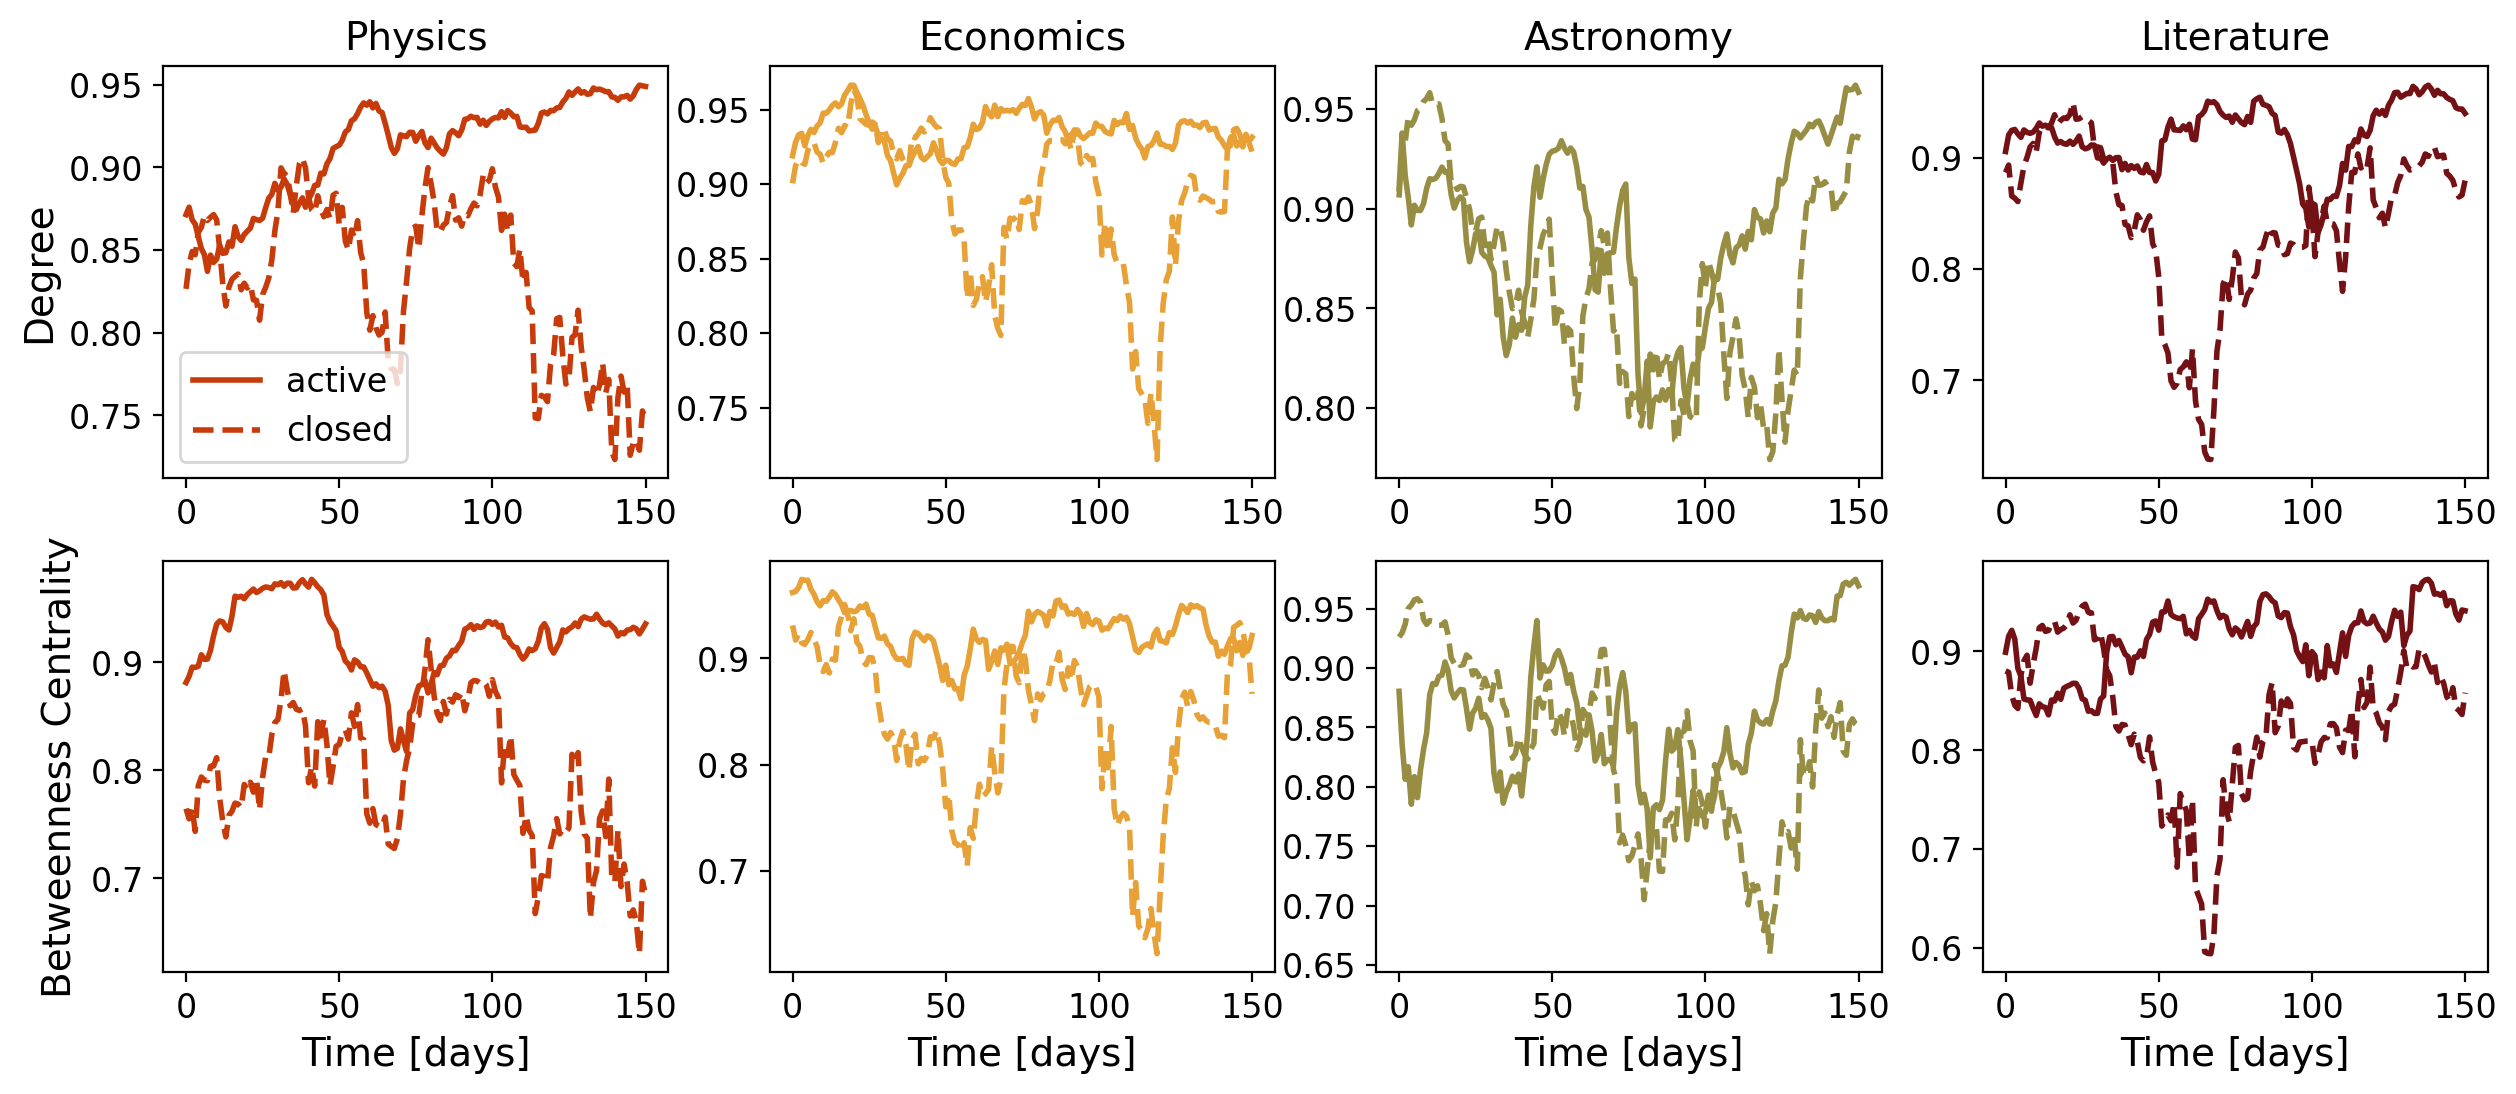
\includegraphics[width=\linewidth]{Figures/FigA7.png}
	\caption{Coefficient of correlation between users' Dynamic Reputation and users' network degree (top) and users's betweenness centrality (bottom). Solid lines - active sites; dashed lines - closed sites.}
	\label{fig:dyn_rep_centrality}
\end{figure}
\\~\\
\textbf{Interaction network - correlation in different layers}

\subsection{Core-periphery structure of the interaction networks}

%In the following section, we will give more details about the structure of 30 days interaction networks. For each sub-network using the BSM (Block Stochastic Model) algorithm, we detected the core and periphery. 

In Q-A communities are common two types of users: popular and casual users. Popular users tend to generate the majority of interactions - they are likely to post more questions, also take part in answering questions and tend to engage discussions through comments. For popular users we consider $10 $  of most active users. We analyse interactions between popular and casual users and  among popular users in the  sub-networks of 30 days [t+30). In both cases the number of links per nodes in active sites are larger than in closed communities (figure \ref{fig:pop_cas_users}).

Although this separation of users puts an emphasis on  differences between closed and active sites, it does not guarantee that all popular users are in the top 10 . To solve this dilemma we use the SBM (Stochastic Block Model) algorithm) to detect the core and the periphery of each 30 days sub-network. Such a split of users leads us to similar conclusions as before. (see figure \ref{fig:windows} - 2nd column)

Stochastic models start from random configuration and the algorithm  can converge to different local stable states. For each 30 days sub-network we run 50 iterations of SBM and choose the model parameters $\theta, p$ according to minimum description length. As example we show analysis of inferred sample of  core-periphery structures for 30 days area51 astronomy networks, Figure \ref{fig:sample}. We represent mean minimum description length (MDL) and mean number of nodes in the core with standard deviation. MDL does not change much among inferred core-periphery structures, still difference between obtained configurations is notable in the number of nodes in the core.  To investigate in more details similarity between obtained core-periphery configurations in the sample we calculate several measures between pair-wised partitions such as normalized mutual information, adjusted rand index, F1 measure and Jaccard index. Those measures are larger than 0.5, and in most cases higher than 0.9 indicating stability of the inferred core-periphery structures.
%TODO
%. MDL does not change much among infered core-periphery structure, Fig \ref{fig:sample} while looking into adjusted rand index we can notice that difference exists. Still, ARI between pair-wised compared partitions is large ($ari >0.9$) indicating stability of inferred structures.    

\begin{figure}
	\centering
	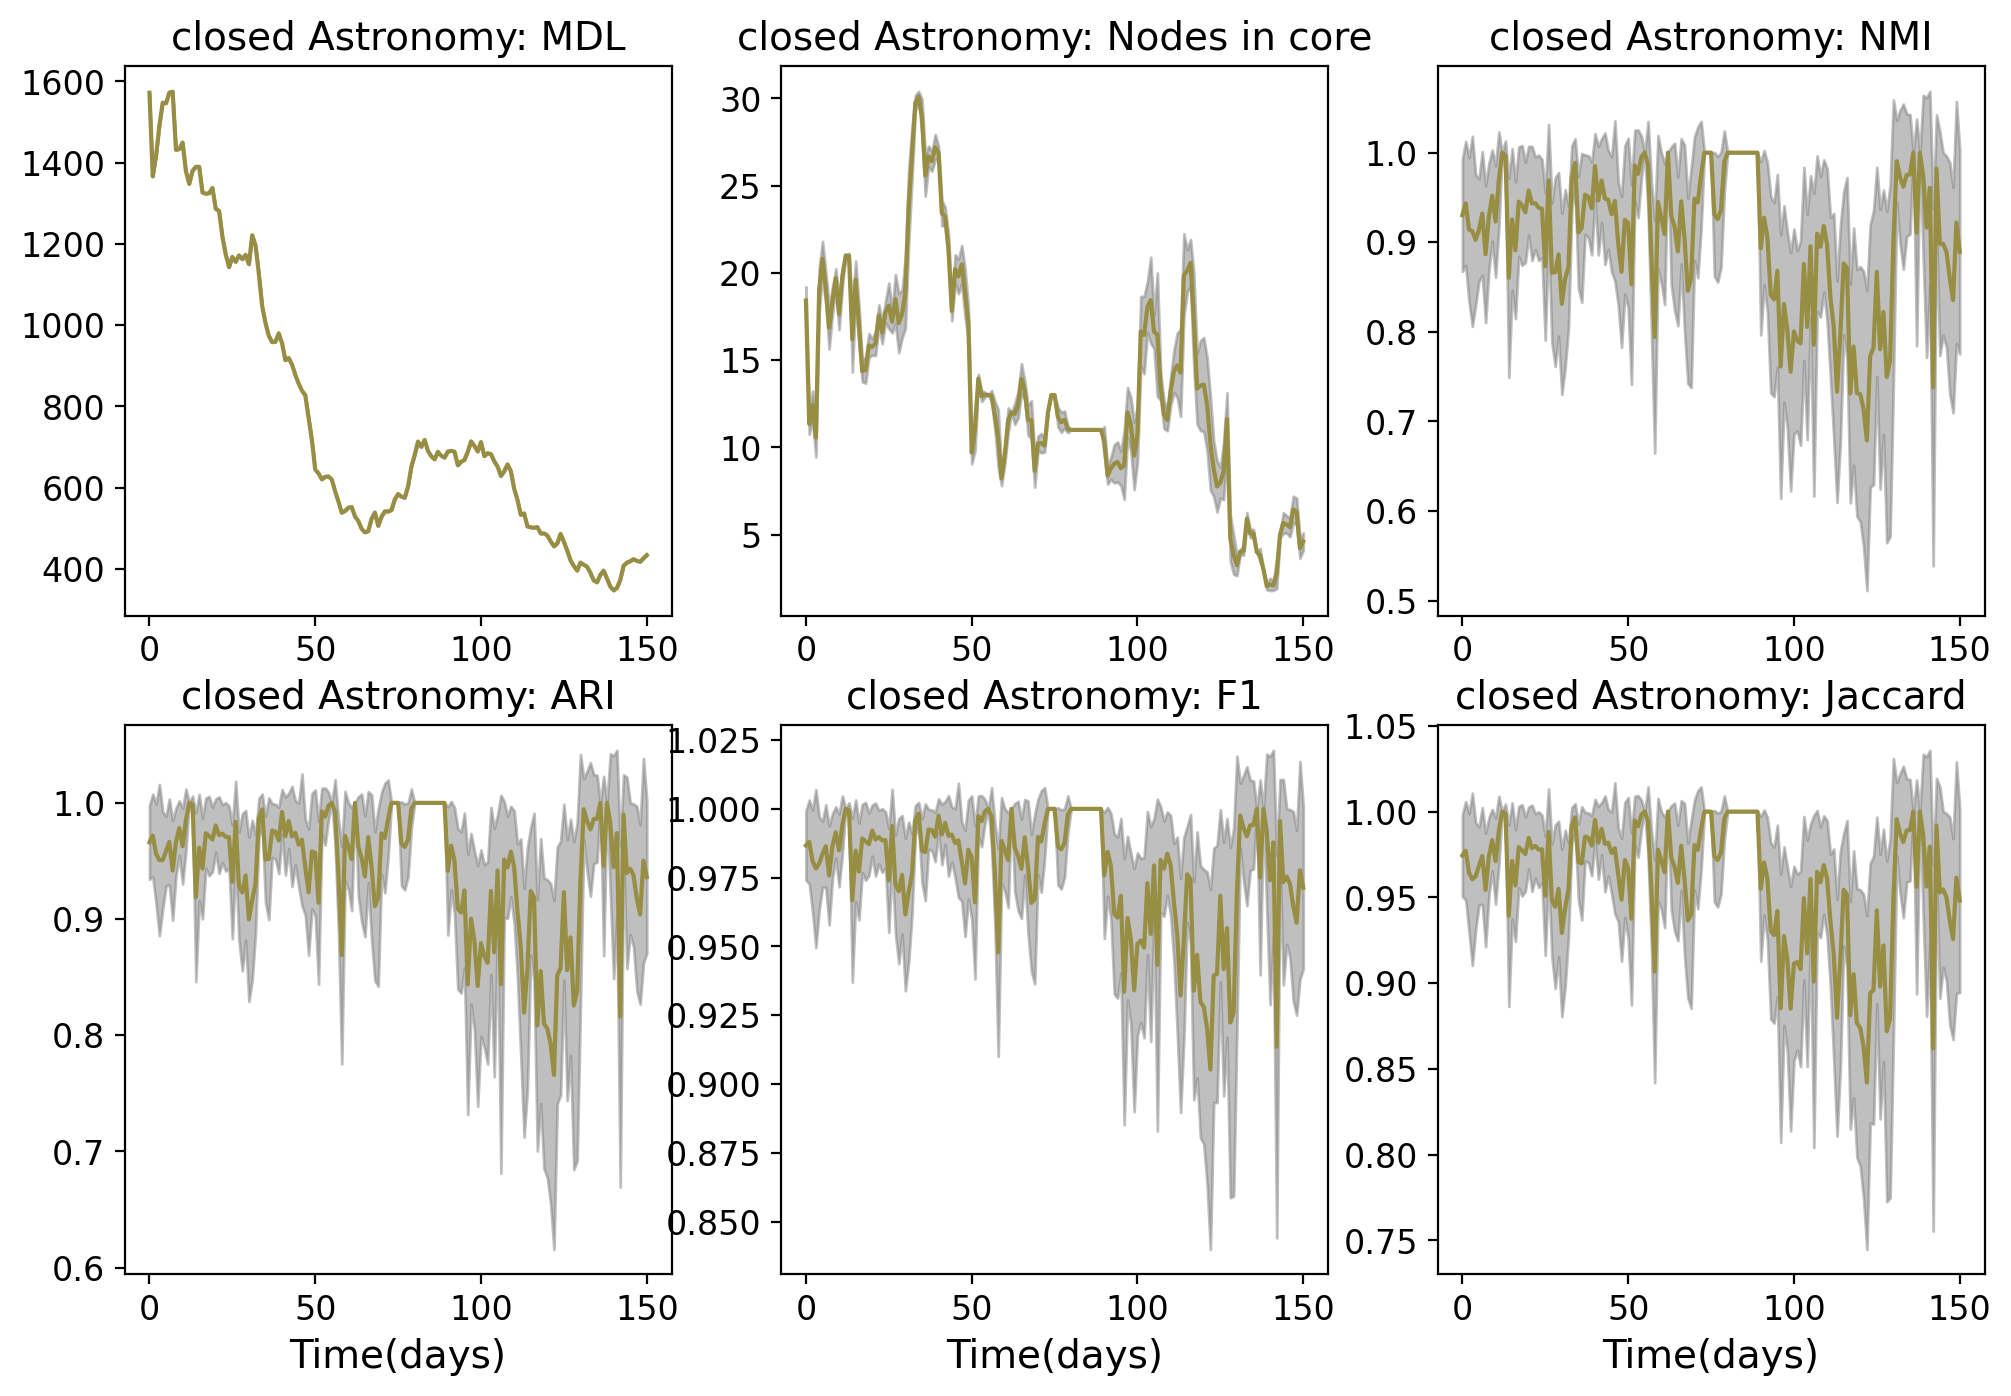
\includegraphics[width=0.8\linewidth]{Figures/FigA8.png}
	\caption{Minimum description lenght, number of nodes in core, normalized mutual information, adjusted rand index, F1 measure and Jaccard index, among 50 samples for 30days sub-networks. Results are given for closed astronomy. }
	\label{fig:sample}
\end{figure}


To study the stability of the core across the time we compute Jaccard’s coefficient between core users in [t+30) networks selected at times $t_1$ and $t_2$, (figure \ref{fig:jaccard_hm}). Higher values of the Jaccard index indicate that core users tend to stay in the core. The detected cores experience a lot of change over time and the highest overlap between core users is in the network closer in the time. The average Jaccard index between core users in all sub-networks separated by time interval $|t_1 - t_2|$ with standard deviation confidence interval is presented in figure \ref{fig:jaccard_mean}. Compared to closed sites, active sites show more stability in the core. Even the number of core users obtained in the launched and closed communities are comparable \ref{fig:core_size} (a high difference is found only for physics ), the ratio between total core and periphery reputation is evidently higher in the active than in closed sites, figure \ref{fig:dr_core_per}.  

\begin{figure}[h!]
	\centering
	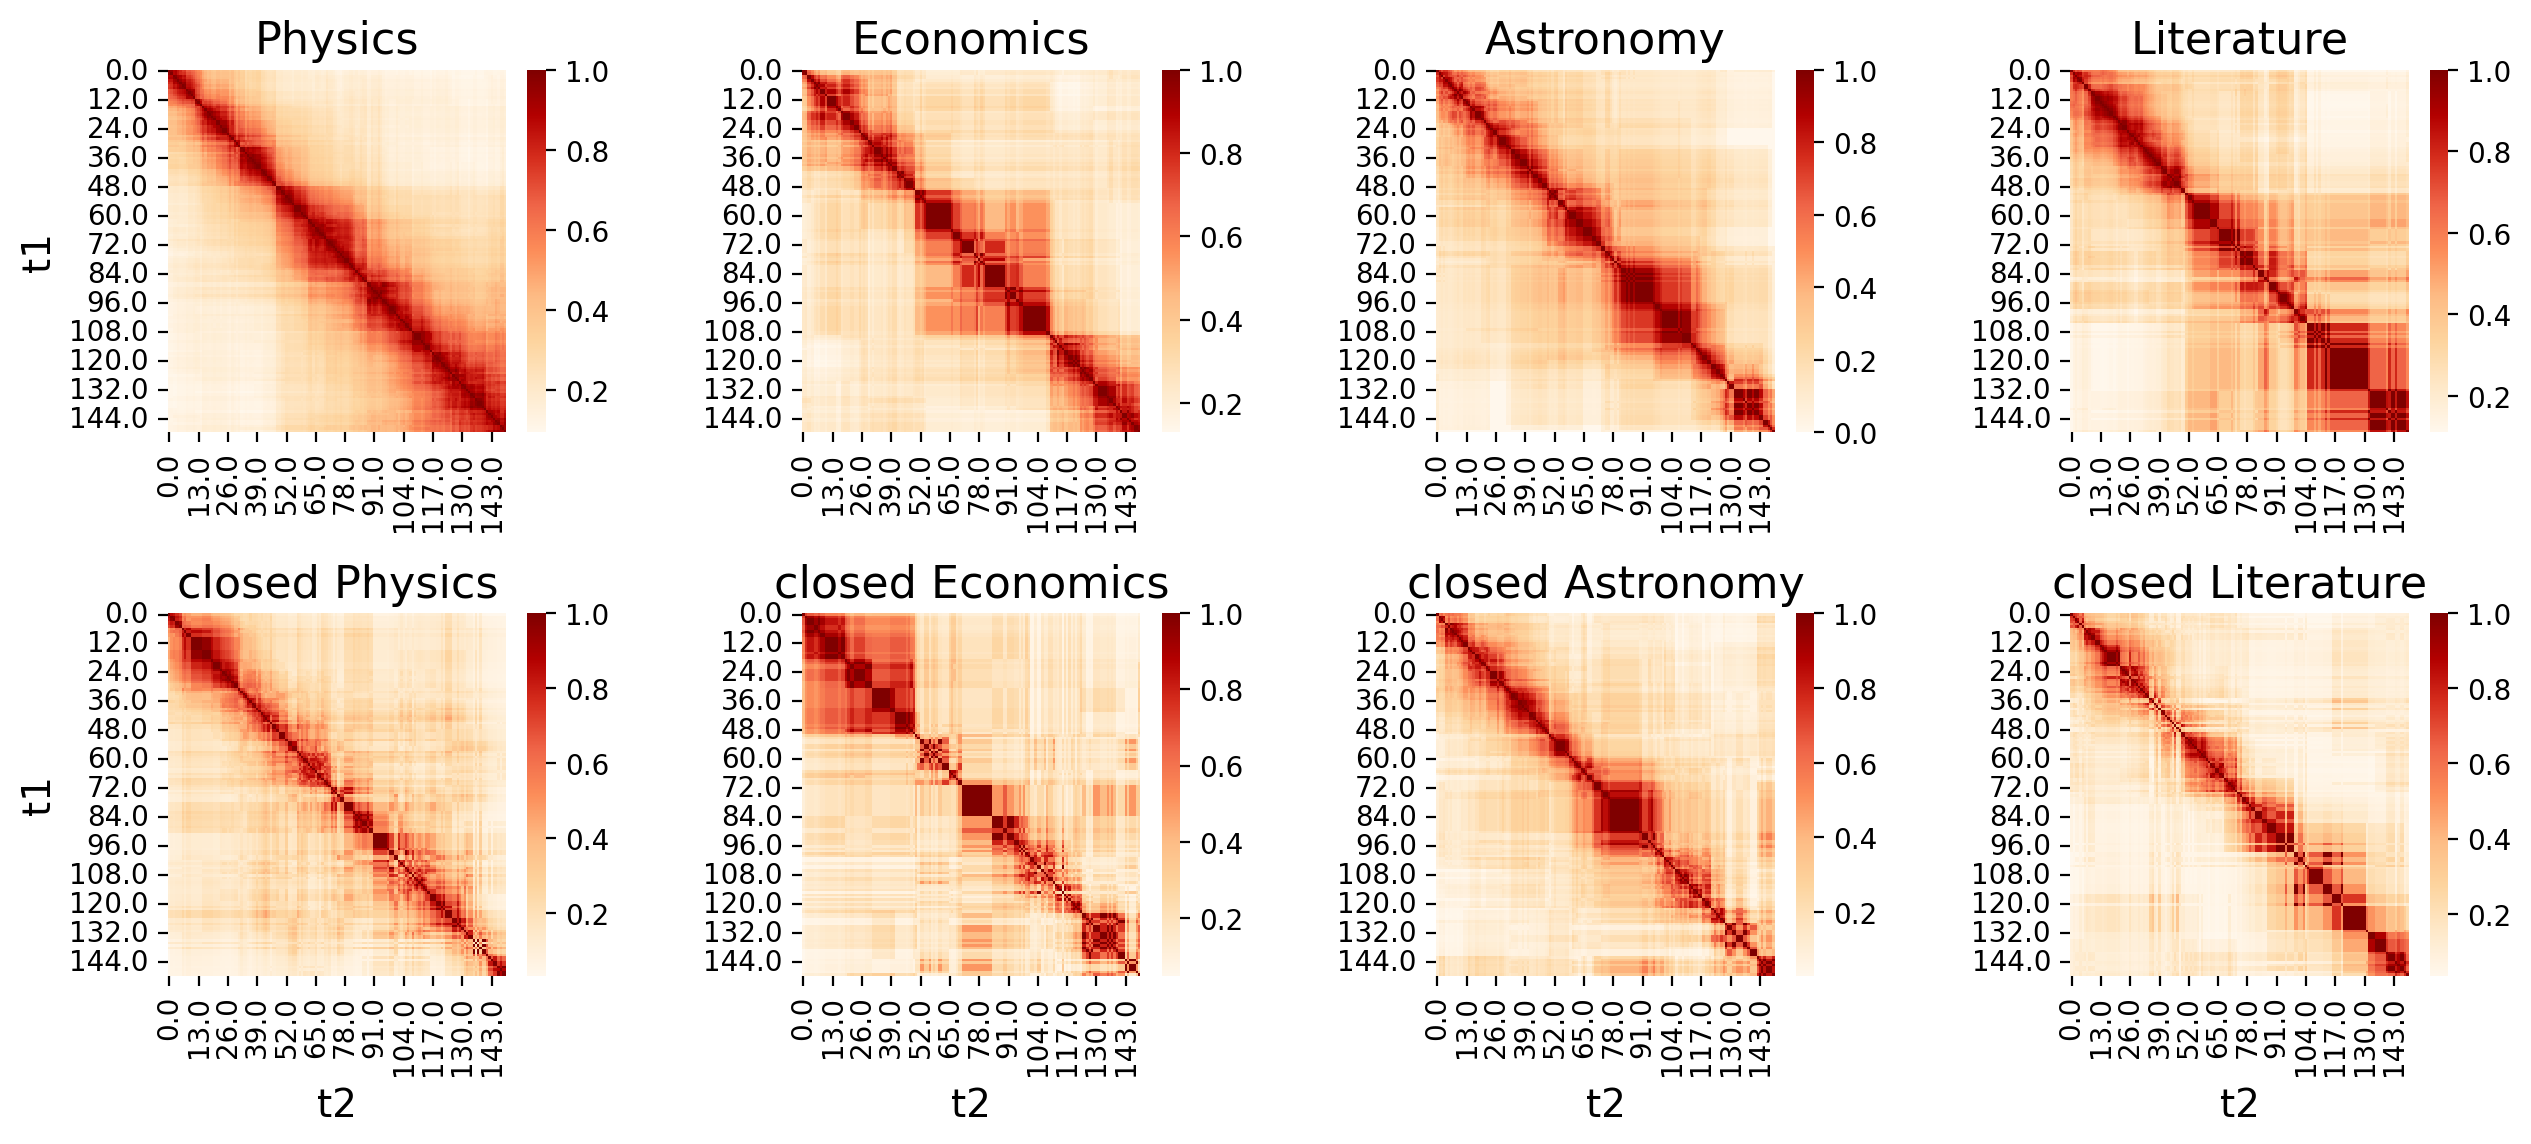
\includegraphics[width=\linewidth]{Figures/FigA10.png}
	\caption{Jaccard index between core users in  sub-networks at time points $t1$ and $t2$}
	\label{fig:jaccard_hm}
\end{figure}

\begin{figure}[h!]
	\centering
	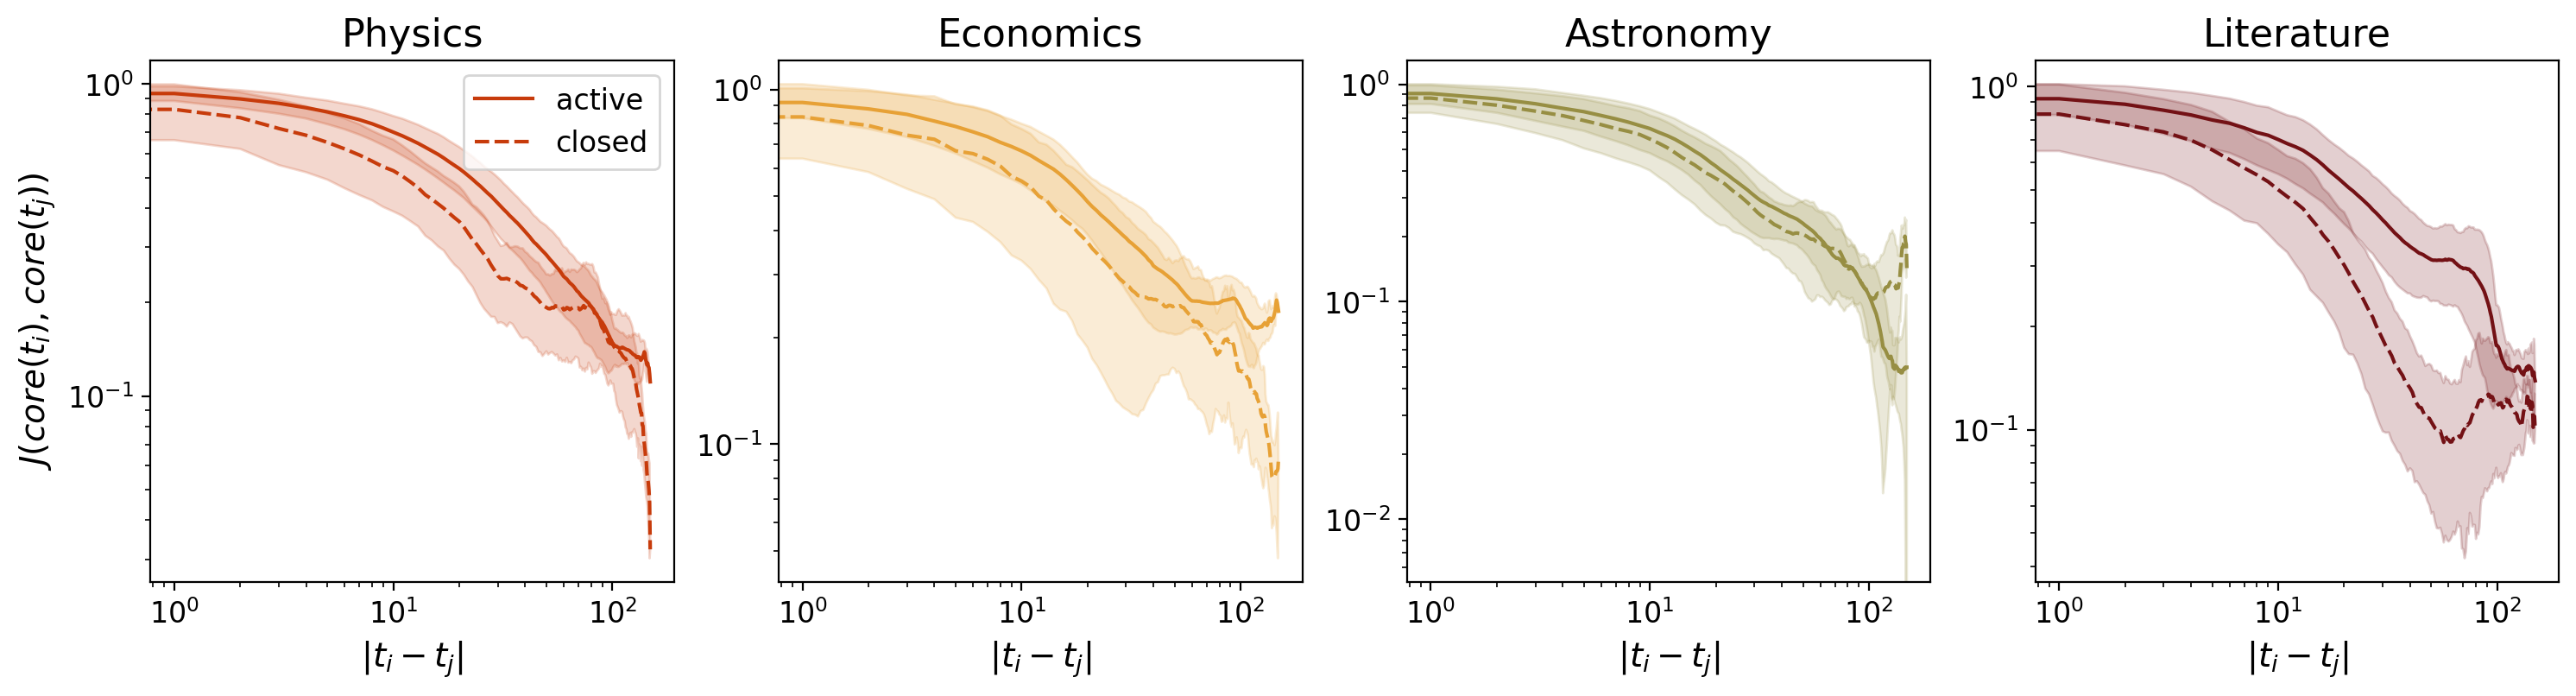
\includegraphics[width=\linewidth]{Figures/FigA9.png}
	\caption{Jaccard index between core users in 30days sub-networks for all possible pairs of 30 days sub-networks separated by time interval $|t_i - t_j|$}
	\label{fig:jaccard_mean}
\end{figure}

% mozda bi ove dve slike core size i ration between reputations mogli da spojimo (slike A9 i A10), samo da se doda treci red na A9? 

\begin{figure}[h!]
	\centering
	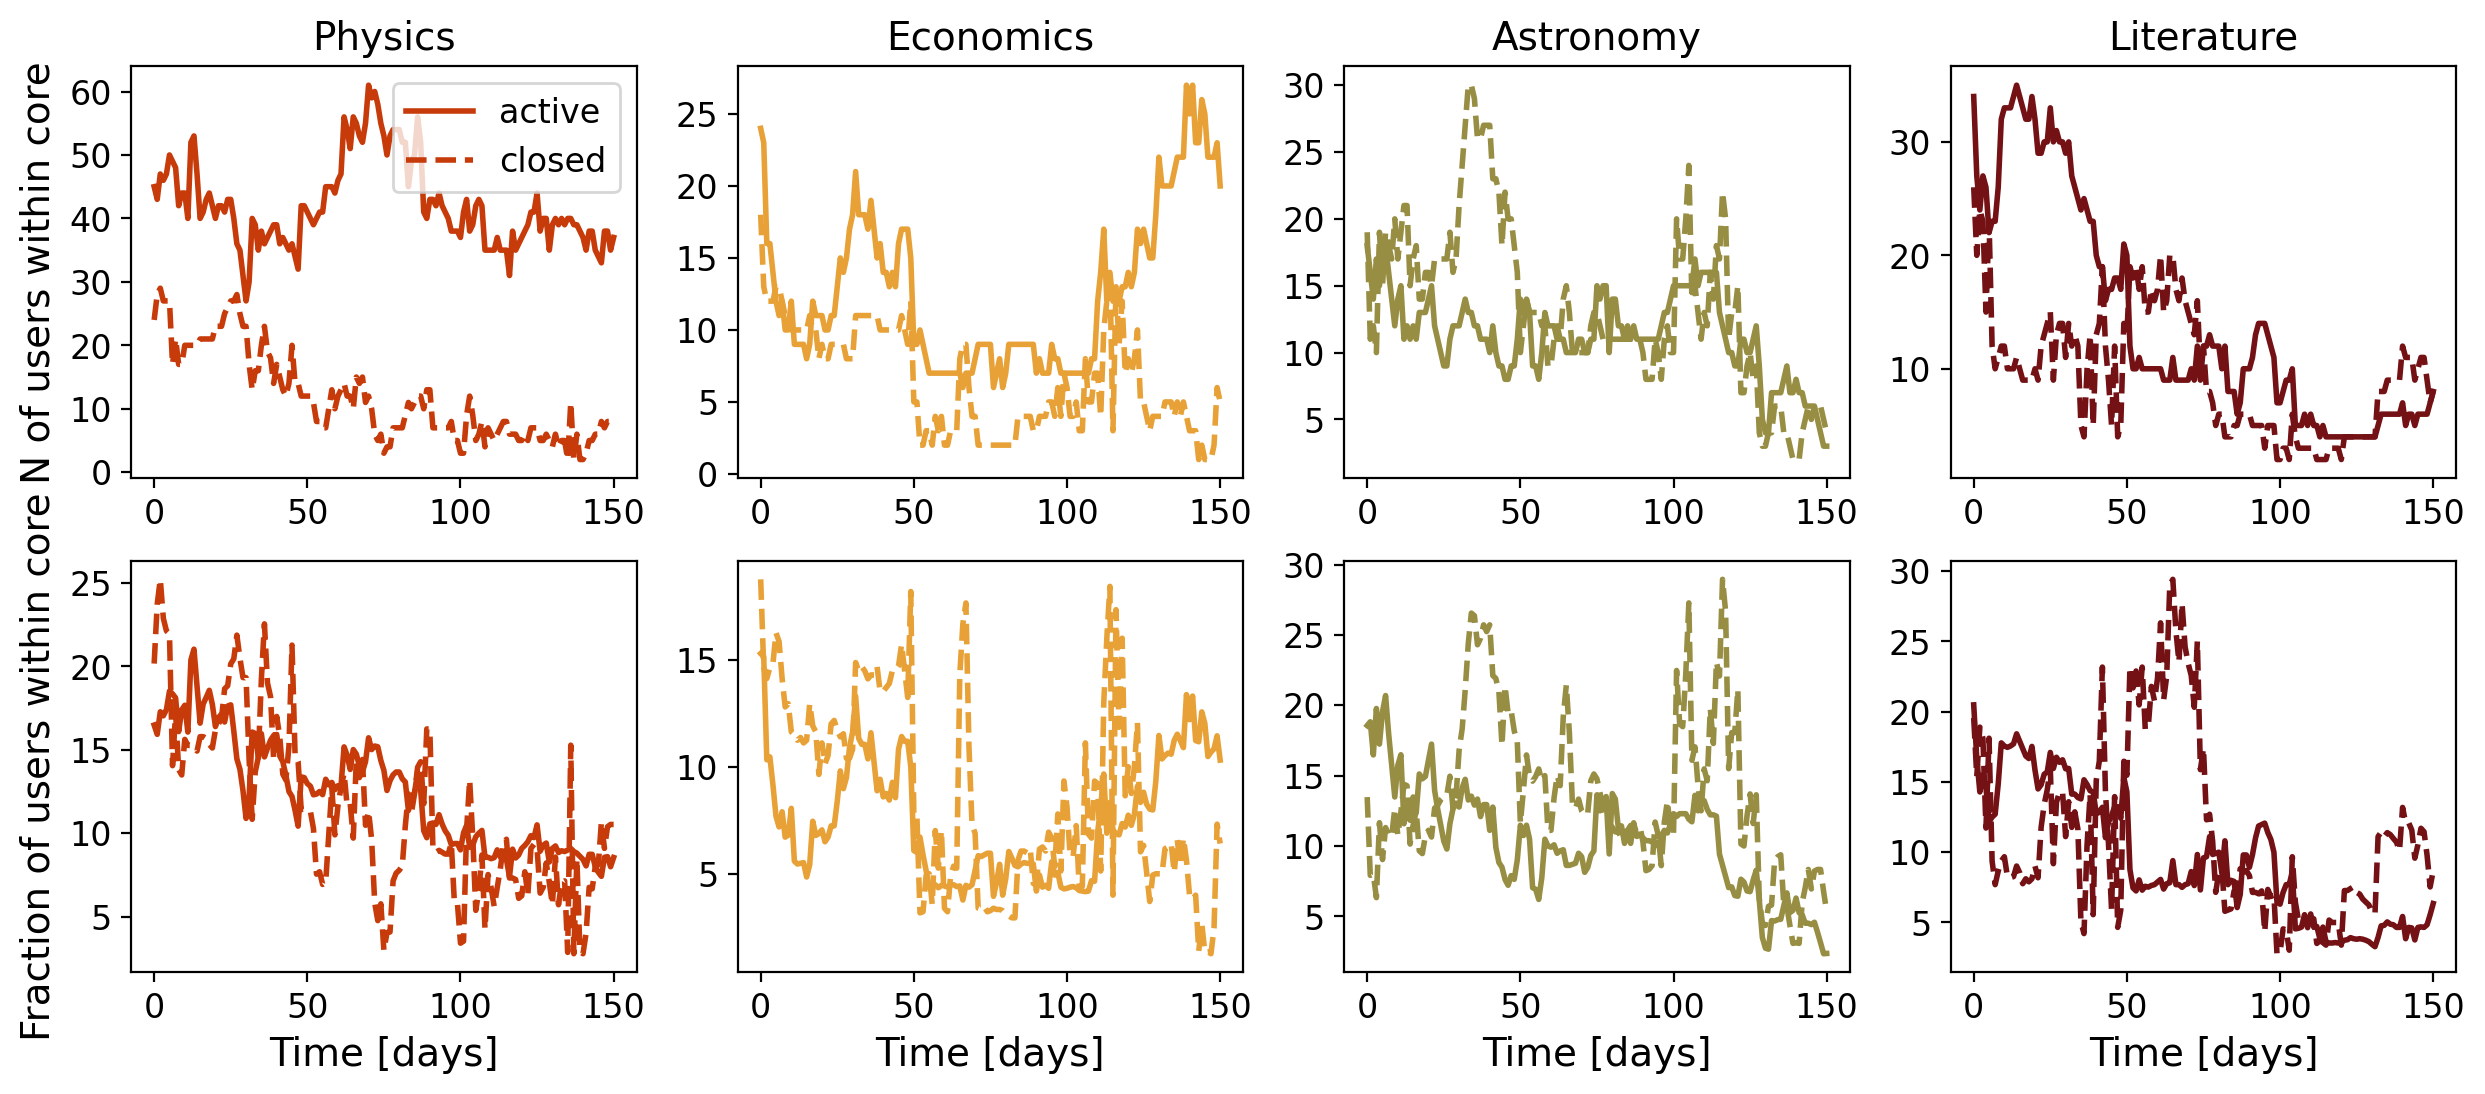
\includegraphics[width=\linewidth]{Figures/FigA11.png}
	\caption{Just for reference size of the core (top) and fraction of users in core (bottom). Solid lines - active sites; dashed lines - closed sites.}
	\label{fig:core_size}
\end{figure}

\begin{figure}[h!]
	\centering
	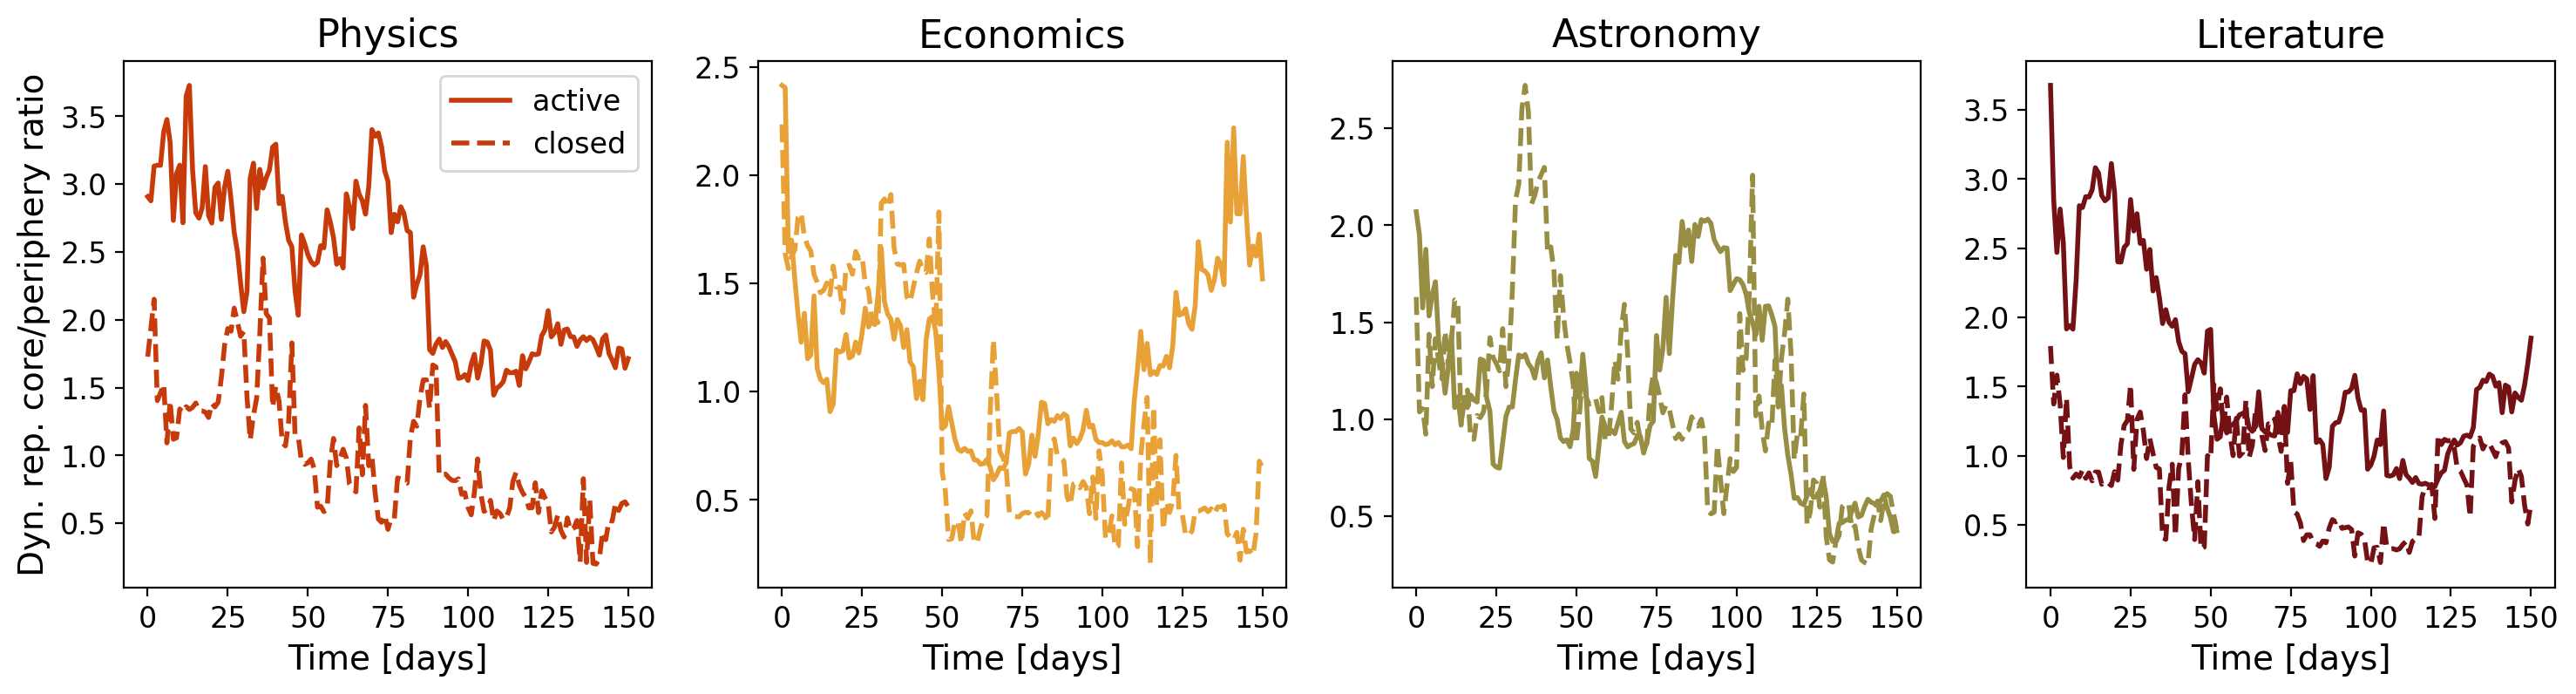
\includegraphics[width=\linewidth]{Figures/FigA12.png}
	\caption{Ratio between the total reputation within network core and periphery. Solid lines beta communities, dashed lines area 51 communities.}
	\label{fig:dr_core_per}
\end{figure}

\clearpage
\begin{figure}[h!]
	\centering
	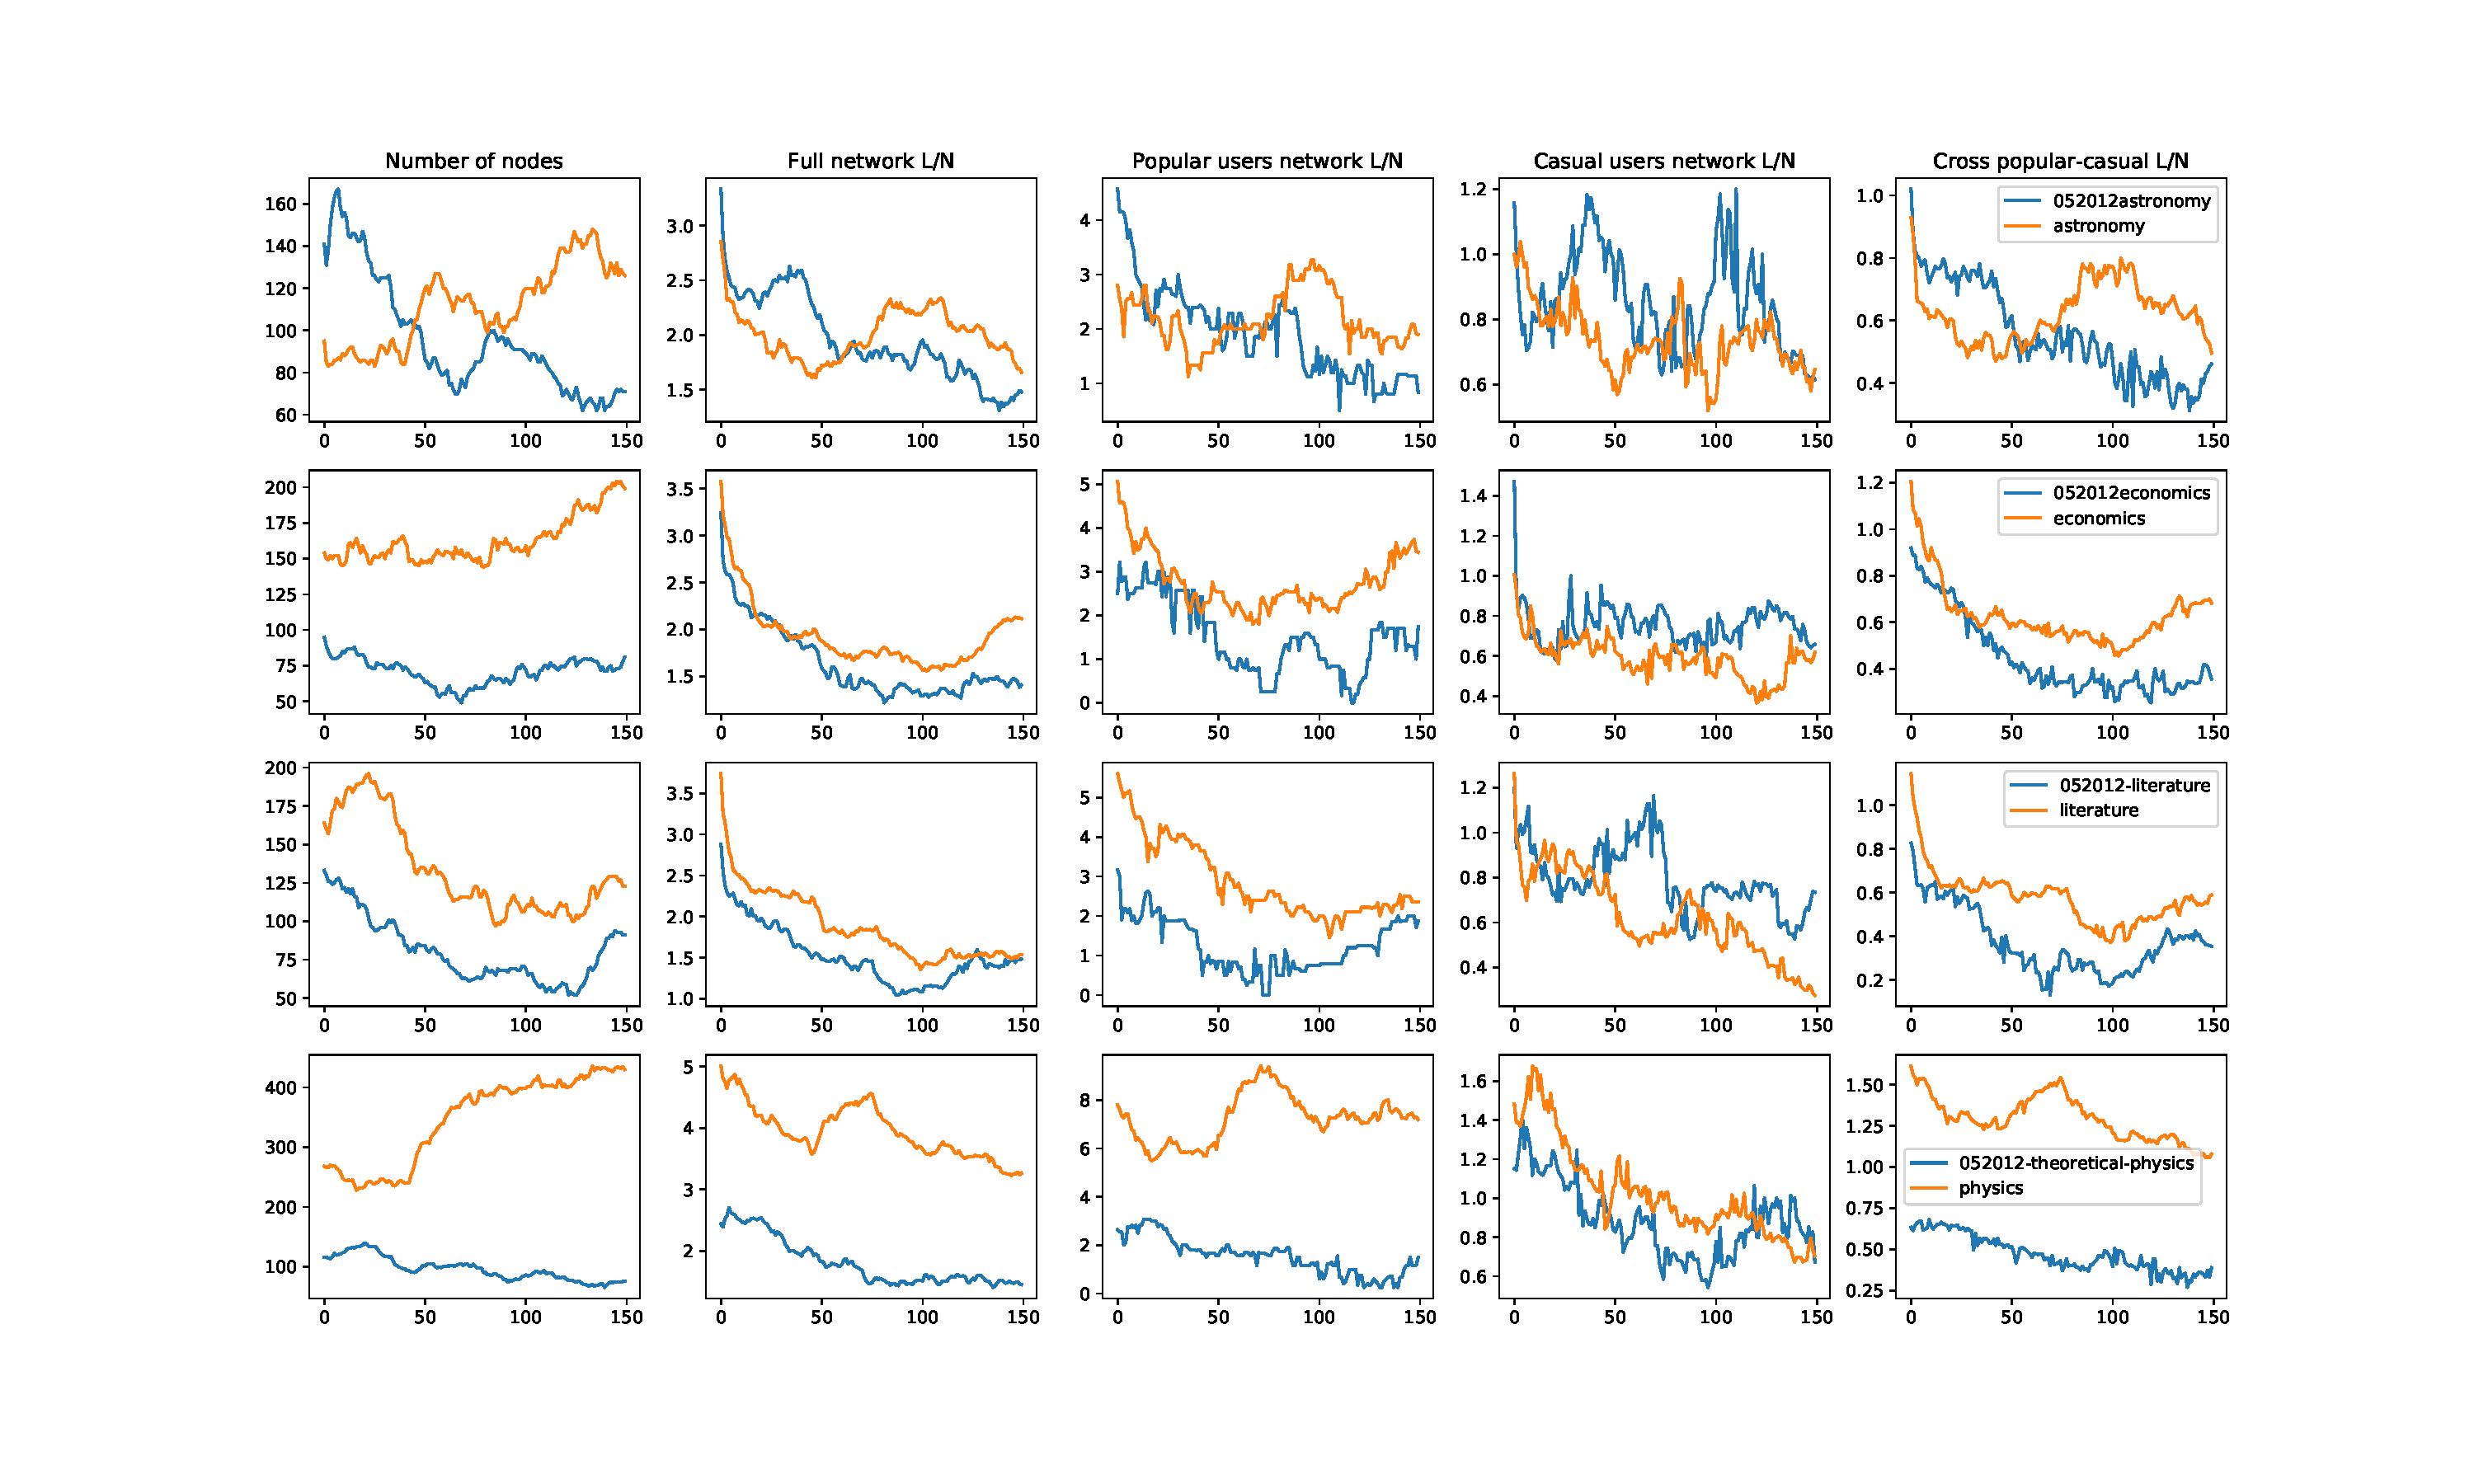
\includegraphics[width=\linewidth]{Figures/popular_casual_degree_interactions_top10.pdf}
	\caption{Links per node among popular users (top 10\% of users) and between popular and casual users (everyone but popular users).
		Reminder: only 3rd and 5th columns should stay and only for reference to previous research, while our point is to this selection via core/periphery decomposition without thresholding.}
	\label{fig:pop_cas_users}
\end{figure}

\subsection{The choice of the sliding window}

In this section, we investigate how the size of sliding windows affect network properties over time. Figure \ref{fig:windows} summarize results for one pair of communities, area51 and beta astronomy, but similar conclusions can be observed for other pairs of sites. We show the network properties for sub-networks of 10, 30, and 60 days sliding windows. For a sliding window of 10 days, results may be too noisy and we may not observe some important trends in the community. The number of users for beta astronomy seems to fluctuate around some mean value. On the larger scale, 30 days window,  it is more clear that the number of users slightly increase over time. Contrary, for too large an aggregation window (60 days), important information about the time series can be lost, such as the local minimum of the number of users around time step 80 that is observed for the 30-day sliding window. Looking into other network characteristics such as L/N and clustering we conclude that differences between closed and  active sites are more transparent with a larger aggregation window, still, on each scale, beta sites show a higher number of nodes, number of links per node and clustering coefficient.

As before we study the structure of created sub-networks through the lens of core-periphery structure. On small scales, the window of 10 days, there are often few, or even no nodes in the core and it can affect the calculation of other measures of interest. Such behaviour is more typical for closed communities.  With the size of the sliding window number of nodes in the core increases and results of core-periphery measures %in the number of nodes, L/N in the core, L/N between core-periphery and dynamical reputation between core users and between core and periphery users 
become smoother. Finally, the choice of the sliding window does not change conclusions that core users in the beta communities produce more activity and make the strong core. However, our main results are shown for a sliding window of 30 days, as it makes a good compromise between large and small time scales.  


\begin{figure}[h!]
	\centering
	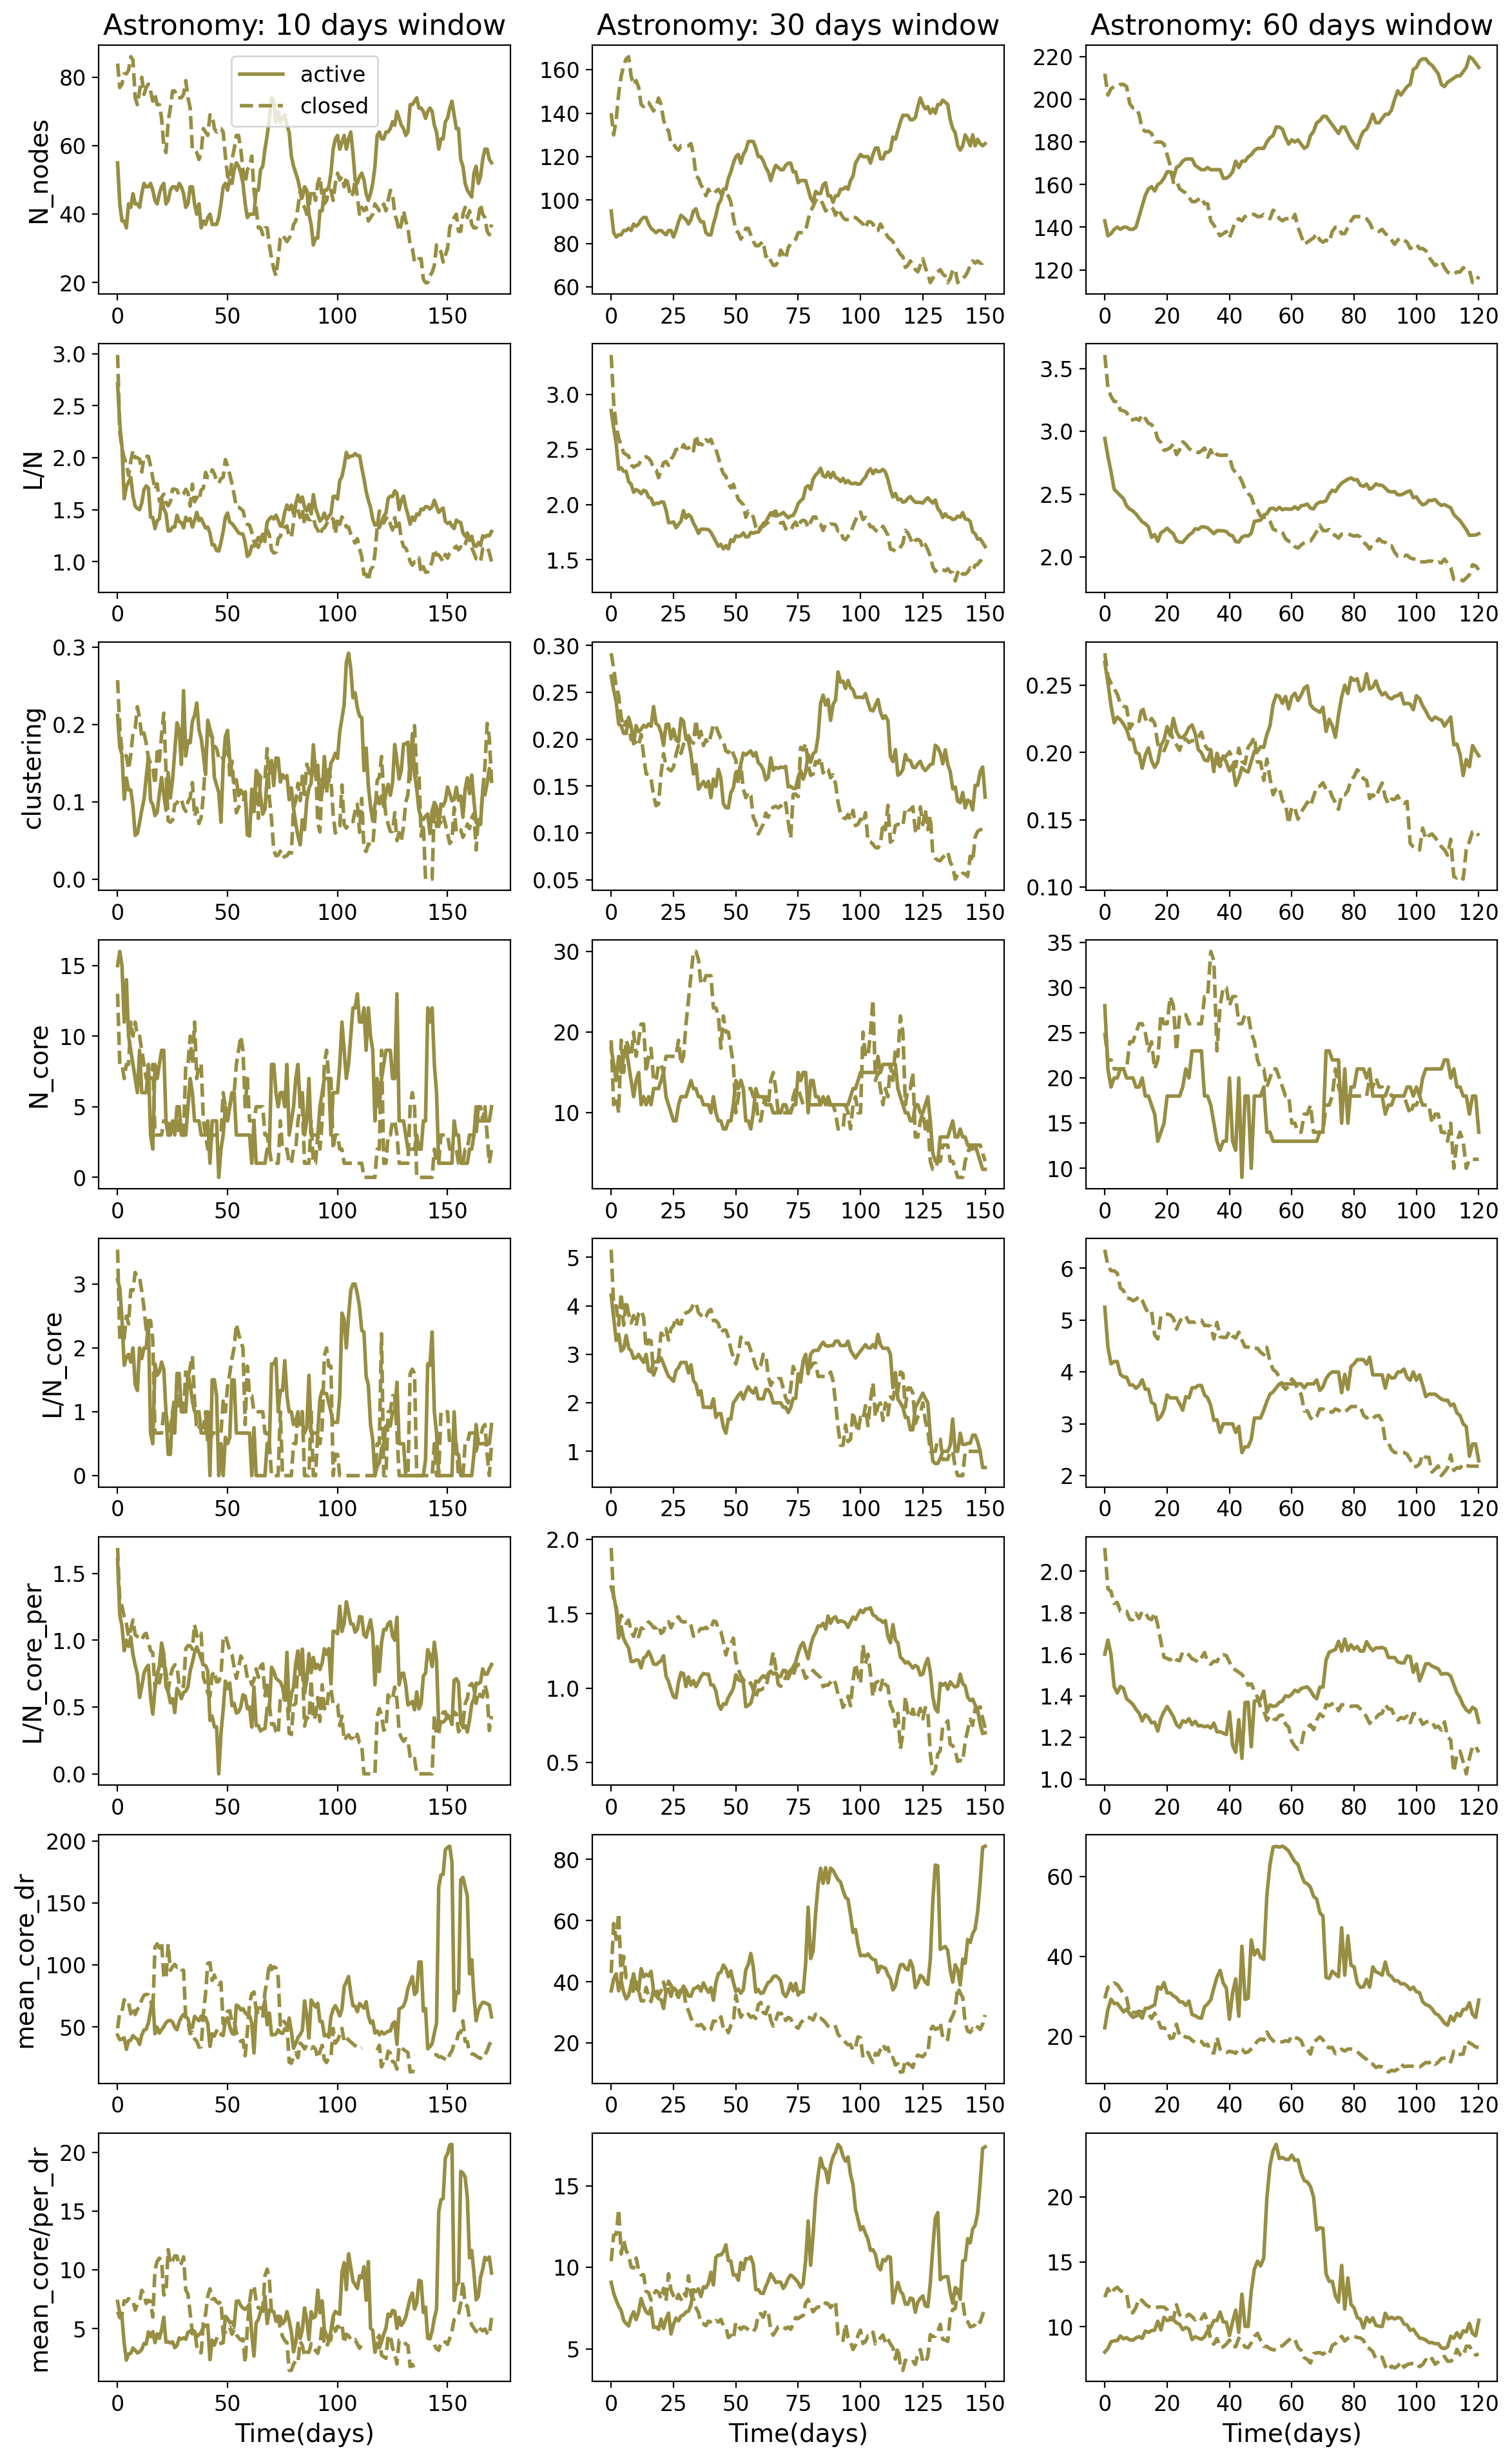
\includegraphics[width=0.8\linewidth]{Figures/FigA14}
	\caption{Results for different sliding windows. Example is for astronomy, blue solid lines- active, orange dashed lines - closed site. }
	\label{fig:windows}
	% Ovo je mozda previse grafika, pa je mozda podeliti na dva dela. 
	% Ovo je primer za astronomiju (ali ako se odlucimo za neku drugu moze se zameniti)
\end{figure}



       


% The back matter includes commands to produce endnotes, index,
% glossary, bibiliography, and the like.

%\backmatter

%\printpagenotes
\bibliography{sample-thesis.bib}
\bibliographystyle{unsrt}





% The appendix contains material that would clutter up the main text,
% such as program code, survey instruments, or interview transcripts.
% Remove it if you don't have an appendix.

%\appendix

%% Sample University of Calgary Thesis
% This file contains the APPENDIX

% If there is just one appendix, it must be called ``Appendix.'' For
% multiple appendices, use \chapter and a descriptive title,
% e.g., \chapter{Questionnaires}

\chapter*{Appendix}\label{appendix}

% \chapter* doesn't include it in the TOC, so we have to do that by
% hand.  If you have multiple appendices, use \chapter instead and
% remove the following line. 

\addcontentsline{toc}{chapter}{Appendix}

An appendix is a way to include important information that would
otherwise clutter up your thesis. It should be included when there is
additional relevant information that won't fit in the body of your
thesis. Any Appendix must also be mentioned in the body of your thesis
(e.g., ``For a full list of interview questions used, please see the
\hyperref[appendix]{Appendix}''). If your thesis only has one appendix, it
must be titled ``Appendix.'' If your thesis has more than one appendix,
add alphabetized letters, starting with ``Appendix~A.'' The following
are examples of things you might include in appendices:
\begin{enumerate}
  \item Copyright permissions with signatures removed
  \item Additional details of methodology and/or data
  \item Diagrams of equipment that you developed
  \item Digital files and/or artwork digital models
  \item Blank copies of questionnaires or surveys used in your research
\end{enumerate}

\printbibliography  

\end{document}
